% Options for packages loaded elsewhere
\PassOptionsToPackage{unicode}{hyperref}
\PassOptionsToPackage{hyphens}{url}
\PassOptionsToPackage{dvipsnames,svgnames,x11names}{xcolor}
%
\documentclass[
  letterpaper,
  DIV=11,
  numbers=noendperiod]{scrreprt}

\usepackage{amsmath,amssymb}
\usepackage{iftex}
\ifPDFTeX
  \usepackage[T1]{fontenc}
  \usepackage[utf8]{inputenc}
  \usepackage{textcomp} % provide euro and other symbols
\else % if luatex or xetex
  \usepackage{unicode-math}
  \defaultfontfeatures{Scale=MatchLowercase}
  \defaultfontfeatures[\rmfamily]{Ligatures=TeX,Scale=1}
\fi
\usepackage{lmodern}
\ifPDFTeX\else  
    % xetex/luatex font selection
\fi
% Use upquote if available, for straight quotes in verbatim environments
\IfFileExists{upquote.sty}{\usepackage{upquote}}{}
\IfFileExists{microtype.sty}{% use microtype if available
  \usepackage[]{microtype}
  \UseMicrotypeSet[protrusion]{basicmath} % disable protrusion for tt fonts
}{}
\makeatletter
\@ifundefined{KOMAClassName}{% if non-KOMA class
  \IfFileExists{parskip.sty}{%
    \usepackage{parskip}
  }{% else
    \setlength{\parindent}{0pt}
    \setlength{\parskip}{6pt plus 2pt minus 1pt}}
}{% if KOMA class
  \KOMAoptions{parskip=half}}
\makeatother
\usepackage{xcolor}
\setlength{\emergencystretch}{3em} % prevent overfull lines
\setcounter{secnumdepth}{5}
% Make \paragraph and \subparagraph free-standing
\ifx\paragraph\undefined\else
  \let\oldparagraph\paragraph
  \renewcommand{\paragraph}[1]{\oldparagraph{#1}\mbox{}}
\fi
\ifx\subparagraph\undefined\else
  \let\oldsubparagraph\subparagraph
  \renewcommand{\subparagraph}[1]{\oldsubparagraph{#1}\mbox{}}
\fi


\providecommand{\tightlist}{%
  \setlength{\itemsep}{0pt}\setlength{\parskip}{0pt}}\usepackage{longtable,booktabs,array}
\usepackage{calc} % for calculating minipage widths
% Correct order of tables after \paragraph or \subparagraph
\usepackage{etoolbox}
\makeatletter
\patchcmd\longtable{\par}{\if@noskipsec\mbox{}\fi\par}{}{}
\makeatother
% Allow footnotes in longtable head/foot
\IfFileExists{footnotehyper.sty}{\usepackage{footnotehyper}}{\usepackage{footnote}}
\makesavenoteenv{longtable}
\usepackage{graphicx}
\makeatletter
\def\maxwidth{\ifdim\Gin@nat@width>\linewidth\linewidth\else\Gin@nat@width\fi}
\def\maxheight{\ifdim\Gin@nat@height>\textheight\textheight\else\Gin@nat@height\fi}
\makeatother
% Scale images if necessary, so that they will not overflow the page
% margins by default, and it is still possible to overwrite the defaults
% using explicit options in \includegraphics[width, height, ...]{}
\setkeys{Gin}{width=\maxwidth,height=\maxheight,keepaspectratio}
% Set default figure placement to htbp
\makeatletter
\def\fps@figure{htbp}
\makeatother

\KOMAoption{captions}{tableheading}
\makeatletter
\@ifpackageloaded{tcolorbox}{}{\usepackage[skins,breakable]{tcolorbox}}
\@ifpackageloaded{fontawesome5}{}{\usepackage{fontawesome5}}
\definecolor{quarto-callout-color}{HTML}{909090}
\definecolor{quarto-callout-note-color}{HTML}{0758E5}
\definecolor{quarto-callout-important-color}{HTML}{CC1914}
\definecolor{quarto-callout-warning-color}{HTML}{EB9113}
\definecolor{quarto-callout-tip-color}{HTML}{00A047}
\definecolor{quarto-callout-caution-color}{HTML}{FC5300}
\definecolor{quarto-callout-color-frame}{HTML}{acacac}
\definecolor{quarto-callout-note-color-frame}{HTML}{4582ec}
\definecolor{quarto-callout-important-color-frame}{HTML}{d9534f}
\definecolor{quarto-callout-warning-color-frame}{HTML}{f0ad4e}
\definecolor{quarto-callout-tip-color-frame}{HTML}{02b875}
\definecolor{quarto-callout-caution-color-frame}{HTML}{fd7e14}
\makeatother
\makeatletter
\makeatother
\makeatletter
\@ifpackageloaded{bookmark}{}{\usepackage{bookmark}}
\makeatother
\makeatletter
\@ifpackageloaded{caption}{}{\usepackage{caption}}
\AtBeginDocument{%
\ifdefined\contentsname
  \renewcommand*\contentsname{Table of contents}
\else
  \newcommand\contentsname{Table of contents}
\fi
\ifdefined\listfigurename
  \renewcommand*\listfigurename{List of Figures}
\else
  \newcommand\listfigurename{List of Figures}
\fi
\ifdefined\listtablename
  \renewcommand*\listtablename{List of Tables}
\else
  \newcommand\listtablename{List of Tables}
\fi
\ifdefined\figurename
  \renewcommand*\figurename{Figure}
\else
  \newcommand\figurename{Figure}
\fi
\ifdefined\tablename
  \renewcommand*\tablename{Table}
\else
  \newcommand\tablename{Table}
\fi
}
\@ifpackageloaded{float}{}{\usepackage{float}}
\floatstyle{ruled}
\@ifundefined{c@chapter}{\newfloat{codelisting}{h}{lop}}{\newfloat{codelisting}{h}{lop}[chapter]}
\floatname{codelisting}{Listing}
\newcommand*\listoflistings{\listof{codelisting}{List of Listings}}
\makeatother
\makeatletter
\@ifpackageloaded{caption}{}{\usepackage{caption}}
\@ifpackageloaded{subcaption}{}{\usepackage{subcaption}}
\makeatother
\makeatletter
\@ifpackageloaded{tcolorbox}{}{\usepackage[skins,breakable]{tcolorbox}}
\makeatother
\makeatletter
\@ifundefined{shadecolor}{\definecolor{shadecolor}{rgb}{.97, .97, .97}}
\makeatother
\makeatletter
\makeatother
\makeatletter
\makeatother
\ifLuaTeX
  \usepackage{selnolig}  % disable illegal ligatures
\fi
\IfFileExists{bookmark.sty}{\usepackage{bookmark}}{\usepackage{hyperref}}
\IfFileExists{xurl.sty}{\usepackage{xurl}}{} % add URL line breaks if available
\urlstyle{same} % disable monospaced font for URLs
\hypersetup{
  pdftitle={Procedury},
  pdfauthor={Maurycy Żarczyński},
  colorlinks=true,
  linkcolor={blue},
  filecolor={Maroon},
  citecolor={Blue},
  urlcolor={Blue},
  pdfcreator={LaTeX via pandoc}}

\title{Procedury}
\usepackage{etoolbox}
\makeatletter
\providecommand{\subtitle}[1]{% add subtitle to \maketitle
  \apptocmd{\@title}{\par {\large #1 \par}}{}{}
}
\makeatother
\subtitle{Katedra Geomorfologii i Geologii Czwartorzędu}
\author{Maurycy Żarczyński}
\date{}

\begin{document}
\maketitle
\ifdefined\Shaded\renewenvironment{Shaded}{\begin{tcolorbox}[boxrule=0pt, sharp corners, enhanced, breakable, borderline west={3pt}{0pt}{shadecolor}, frame hidden, interior hidden]}{\end{tcolorbox}}\fi

\renewcommand*\contentsname{Table of contents}
{
\hypersetup{linkcolor=}
\setcounter{tocdepth}{2}
\tableofcontents
}
\bookmarksetup{startatroot}

\hypertarget{wstux119p}{%
\chapter*{Wstęp}\label{wstux119p}}
\addcontentsline{toc}{chapter}{Wstęp}

\markboth{Wstęp}{Wstęp}

Zbiór procedur laboratoryjnych i terenowych Katedry Geomorfologii i
Geologii Czwartorzędu.

\begin{figure}

{\centering 
\includegraphics{images/Asset 1@8x.png}

}

\end{figure}

\part{Prace terenowe}

\hypertarget{batymetria}{%
\chapter{Batymetria}\label{batymetria}}

Echosonda Humminbird 385ci

\hypertarget{praca-z-echosondux105}{%
\section{Praca z echosondą}\label{praca-z-echosondux105}}

\begin{itemize}
\tightlist
\item
  Włożyć kartę pamięci SD (SanDisk 16GB w standardzie \textbf{HC1} i z
  systemem plików \textbf{FAT32}).
\end{itemize}

\begin{tcolorbox}[enhanced jigsaw, toptitle=1mm, bottomtitle=1mm, opacitybacktitle=0.6, colframe=quarto-callout-note-color-frame, bottomrule=.15mm, title=\textcolor{quarto-callout-note-color}{\faInfo}\hspace{0.5em}{Karta SD}, colbacktitle=quarto-callout-note-color!10!white, left=2mm, breakable, rightrule=.15mm, colback=white, opacityback=0, arc=.35mm, coltitle=black, leftrule=.75mm, toprule=.15mm, titlerule=0mm]

Karta znajduje się u pracownika technicznego w szufladzie biurka.

\end{tcolorbox}

\begin{itemize}
\tightlist
\item
  Włączyć echosondę.
\item
  Sonda po znalezieniu pozycji GPS (diagnostyka GPS jest dostępna w
  odpowiednim widoku, klawisz \texttt{View}) rejestruje ślad cały czas,
  ale \textbf{nie zapisuje} go automatycznie na stałe.
\item
  Przed wyłączeniem sondy wejść w \texttt{Menu} i zapisać bieżący ślad
  (nawet jeśli konieczny jest na przykład restart w trakcie pomiarów) --
  bez tego ślad zostanie utracony. Menu dostępne np. w widoku mapy
  (klawisz \texttt{View}).
\item
  Po zapisaniu bieżącego śladu w menu wyeksportować wszystkie dane
  nawigacyjne na kartę SD \texttt{Menu} dostępne np. w widoku mapy
  (klawisz \texttt{View}).
\item
  Wyjąć kartę SD z echosondy.
\end{itemize}

\hypertarget{praca-z-danymi}{%
\section{Praca z danymi}\label{praca-z-danymi}}

\hypertarget{import-danych}{%
\subsection{Import danych}\label{import-danych}}

\hypertarget{dane-z-karty-sd}{%
\subsubsection{Dane z karty SD}\label{dane-z-karty-sd}}

\begin{itemize}
\tightlist
\item
  Podłączyć kartę SD do komputera:

  \begin{itemize}
  \item
    Czytnik kart SD w laptopie.
  \item
    Zewnętrzny czytnik kart SD USB.
  \item
    Przez aparat fotograficzny (np. NIKON na stanie Zakładu).
  \end{itemize}
\item
  Włączyć oprogramowanie HumminbirdPC.
\end{itemize}

\begin{tcolorbox}[enhanced jigsaw, toptitle=1mm, bottomtitle=1mm, opacitybacktitle=0.6, colframe=quarto-callout-note-color-frame, bottomrule=.15mm, title=\textcolor{quarto-callout-note-color}{\faInfo}\hspace{0.5em}{Instalator}, colbacktitle=quarto-callout-note-color!10!white, left=2mm, breakable, rightrule=.15mm, colback=white, opacityback=0, arc=.35mm, coltitle=black, leftrule=.75mm, toprule=.15mm, titlerule=0mm]

Instalator dostępny w lokalizacji:

\emph{Public\textbackslash Sprzęt i
programy\textbackslash Software\textbackslash Humminbird}

\end{tcolorbox}

\begin{itemize}
\tightlist
\item
  W ustawieniach programu wybrać odpowiednie jednostki:

  \begin{itemize}
  \tightlist
  \item
    Głębokość = \textbf{metry.}
  \item
    Współrzędne = \textbf{stopnie} \textbf{z rozwinięciem dziesiętnym}.
  \end{itemize}
\item
  W ustawieniach programu sprawdzić i ustawić odpowiedni katalog
  eksportu plików \texttt{.gpx}.
\item
  Przy ikonie karty kliknąć strzałkę opisaną jako
  \texttt{download\ data}.
\end{itemize}

\hypertarget{dane-na-dysku}{%
\subsubsection{Dane na dysku}\label{dane-na-dysku}}

\begin{itemize}
\tightlist
\item
  \texttt{File} -- \texttt{Open}: znaleźć odpowiedni plik \texttt{.gpx}
\end{itemize}

\hypertarget{praca-z-humminbirdpc}{%
\subsection{Praca z HumminbirdPC}\label{praca-z-humminbirdpc}}

\begin{itemize}
\tightlist
\item
  Rozwinąć drzewko pliku \texttt{.gpx}.
\item
  Rozwinąć \texttt{Tracks} (ślady).
\item
  Wybrać odpowiedni ślad.
\item
  Zaznaczyć pierwszy wiersz:

  \begin{itemize}
  \item
    \texttt{CTRL+A} (zaznaczyć wszystko).
  \item
    \texttt{CTRL+C} (skopiować do schowka).
  \end{itemize}
\end{itemize}

\hypertarget{praca-z-microsoft-excel}{%
\subsection{Praca z Microsoft Excel}\label{praca-z-microsoft-excel}}

\begin{itemize}
\item
  Otworzyć nowy arkusz.
\item
  Zaznaczyć trzy kolumny i ustawić format komórek: \textbf{Tekstowe}.
\item
  W pierwszym wierszu ustawić odpowiednie nagłówki:

  \begin{itemize}
  \tightlist
  \item
    Kolumna \textbf{A}: latitude.
  \item
    Kolumna \textbf{B}: longitude.
  \item
    Kolumna \textbf{C}: depth.
  \end{itemize}
\item
  Wkleić z opcją \texttt{Uwzględnij\ formatowanie\ docelowe}.
\item
  Skopiować symbol stopni ``\textbf{°}'' z dowolnej komórki.
\item
  Zaznaczyć kolumny \textbf{A} i \textbf{B}.
\item
  \texttt{Znajdź\ i\ zaznacz} - \texttt{Zamień}:

  \begin{itemize}
  \tightlist
  \item
    Usuwanie znaku stopni:

    \begin{itemize}
    \tightlist
    \item
      Znajdź: °.
    \item
      Zamień: pozostawić puste.
    \item
      \texttt{Zamień\ wszystko}.
    \end{itemize}
  \item
    Usuwanie symbolu szerokości geograficznej:

    \begin{itemize}
    \tightlist
    \item
      Znajdź: N.
    \item
      Zamień: pozostawić puste.
    \item
      \texttt{Zamień\ wszystko}.
    \end{itemize}
  \item
    Usuwanie symbolu długości geograficznej:

    \begin{itemize}
    \tightlist
    \item
      Znajdź: E.
    \item
      Zamień: pozostawić puste.
    \item
      \texttt{Zamień\ wszystko}.
    \end{itemize}
  \item
    Dla kolumny \textbf{longitude} (\textbf{B}) usunąć poprzedzające
    zero:

    \begin{itemize}
    \tightlist
    \item
      Znajdź: 014 (albo inna wartość, zależnie od stopni).
    \item
      Zamień: 14 (albo inna wartość, zależnie od stopni).
    \item
      \texttt{Zamień\ wszystko}.
    \end{itemize}
  \item
    Dla wszystkich kolumn (\textbf{ABC}):

    \begin{itemize}
    \item
      Znajdź: .
    \item
      Zamień: ,
    \item
      \texttt{Zamień\ wszystko}.
    \end{itemize}
  \end{itemize}
\item
  Utworzyć arkusz META.

  Zapisać metadane dotyczące echosondy, daty pomiarów, osób prowadzących
  badania i wszystkich innych istotnych informacji.
\item
  Zapisać plik \texttt{.xlsx} z odpowiednią nazwą.
\end{itemize}

\begin{tcolorbox}[enhanced jigsaw, toptitle=1mm, bottomtitle=1mm, opacitybacktitle=0.6, colframe=quarto-callout-note-color-frame, bottomrule=.15mm, title=\textcolor{quarto-callout-note-color}{\faInfo}\hspace{0.5em}{Pliki XLSX}, colbacktitle=quarto-callout-note-color!10!white, left=2mm, breakable, rightrule=.15mm, colback=white, opacityback=0, arc=.35mm, coltitle=black, leftrule=.75mm, toprule=.15mm, titlerule=0mm]

\emph{RRRR-MM-DD\_bathymetry-JJJ-humminbird.xlsx}

\end{tcolorbox}

\begin{itemize}
\tightlist
\item
  Skopiować wyeksportowany wcześniej plik \texttt{.gpx} z odpowiednią
  nazwą.
\end{itemize}

\begin{tcolorbox}[enhanced jigsaw, toptitle=1mm, bottomtitle=1mm, opacitybacktitle=0.6, colframe=quarto-callout-note-color-frame, bottomrule=.15mm, title=\textcolor{quarto-callout-note-color}{\faInfo}\hspace{0.5em}{Pliki GPX}, colbacktitle=quarto-callout-note-color!10!white, left=2mm, breakable, rightrule=.15mm, colback=white, opacityback=0, arc=.35mm, coltitle=black, leftrule=.75mm, toprule=.15mm, titlerule=0mm]

\emph{RRRR-MM-DD\_bathymetry-JJJ-humminbird.gpx}

Kod jeziora musi być tożsamy z kodami wykorzystywanymi do opisu rdzeni.

\end{tcolorbox}

\textbf{Tab. 1.} Opis oznaczeń wykorzystywanych w nazwie pliku.

\begin{longtable}[]{@{}rll@{}}
\toprule\noalign{}
id & kod & znaczenie \\
\midrule\noalign{}
\endhead
\bottomrule\noalign{}
\endlastfoot
1 & RRRR & rok \\
2 & MM & miesiąc \\
3 & DD & dzień \\
4 & JJJ (dowolna długość) & jezioro \\
\end{longtable}

\begin{itemize}
\tightlist
\item
  Skopiować pliki na serwer.
\end{itemize}

\begin{tcolorbox}[enhanced jigsaw, toptitle=1mm, bottomtitle=1mm, opacitybacktitle=0.6, colframe=quarto-callout-note-color-frame, bottomrule=.15mm, title=\textcolor{quarto-callout-note-color}{\faInfo}\hspace{0.5em}{Lokalizacja danych}, colbacktitle=quarto-callout-note-color!10!white, left=2mm, breakable, rightrule=.15mm, colback=white, opacityback=0, arc=.35mm, coltitle=black, leftrule=.75mm, toprule=.15mm, titlerule=0mm]

\emph{ECRLab\textbackslash Data\textbackslash lake\_bathymetry\textbackslash{}\textbf{JJJ}}

\end{tcolorbox}

\newpage{}

\hypertarget{rejestr-zmian}{%
\section{Rejestr zmian}\label{rejestr-zmian}}

01.12.2022, MZ -- wersja inicjalna Quarto.

Maurycy Żarczyński \texttt{r\ Sys.Date()}

\hypertarget{czujnik-tlenu-rozpuszczonego}{%
\chapter{Czujnik tlenu
rozpuszczonego}\label{czujnik-tlenu-rozpuszczonego}}

\begin{figure}

\href{https://geomorfologia.ug.edu.pl}{
\includegraphics[width=1.5625in,height=\textheight]{images/log-ug_pl.png}}

\end{figure}

\textbf{?var:title.proc-tit}

\begin{center}\rule{0.5\linewidth}{0.5pt}\end{center}

\href{https://www.onsetcomp.com/products/data-loggers/u26-001}{HOBO
U26-001}

\hypertarget{obsux142uga-laboratorium}{%
\section{Obsługa: laboratorium}\label{obsux142uga-laboratorium}}

\hypertarget{obsux142uga-teren}{%
\section{Obsługa: teren}\label{obsux142uga-teren}}

\hypertarget{sprzux119t}{%
\subsection{Sprzęt}\label{sprzux119t}}

\begin{itemize}
\tightlist
\item
  Sprzęg
  \href{https://www.onsetcomp.com/products/communications/u-dtw-1}{U-DTW-1
  Waterproof Shuttle},
\end{itemize}

\begin{tcolorbox}[enhanced jigsaw, toptitle=1mm, bottomtitle=1mm, opacitybacktitle=0.6, colframe=quarto-callout-important-color-frame, bottomrule=.15mm, title=\textcolor{quarto-callout-important-color}{\faExclamation}\hspace{0.5em}{Bateria}, colbacktitle=quarto-callout-important-color!10!white, left=2mm, breakable, rightrule=.15mm, colback=white, opacityback=0, arc=.35mm, coltitle=black, leftrule=.75mm, toprule=.15mm, titlerule=0mm]

Upewnić się, że sprzęg działa a baterie nie są wyczerpane.

\end{tcolorbox}

\begin{itemize}
\tightlist
\item
  Łącznik
  \href{https://www.onsetcomp.com/products/replacements/coupler2-c}{U20L,
  U22, U24, U26} (używany też do termistorów),
\item
  Osłonki
  \href{https://www.onsetcomp.com/products/replacements/u26-rdob-1}{DO
  Sensor Cap - U26-RDOB-1} wraz z akcesoriami (zafoliowany pakiet):

  \begin{itemize}
  \tightlist
  \item
    Osłonka (czarne etui),
  \item
    O-ringi,
  \item
    Smar,
  \item
    Chusteczka nasączona alkoholem,
  \end{itemize}
\item
  Tablet terenowy GETAC,
\end{itemize}

\begin{tcolorbox}[enhanced jigsaw, toptitle=1mm, bottomtitle=1mm, opacitybacktitle=0.6, colframe=quarto-callout-important-color-frame, bottomrule=.15mm, title=\textcolor{quarto-callout-important-color}{\faExclamation}\hspace{0.5em}{Tablet}, colbacktitle=quarto-callout-important-color!10!white, left=2mm, breakable, rightrule=.15mm, colback=white, opacityback=0, arc=.35mm, coltitle=black, leftrule=.75mm, toprule=.15mm, titlerule=0mm]

\begin{itemize}
\tightlist
\item
  Naładować urządzenie przed podróżą,
\item
  Włączyć tablet i upewnić się, że oprogramowanie HOBOware PRO działa
  (instalacja ulega losowemu uszkodzeniu po niektórych aktualizacjach).
\end{itemize}

\end{tcolorbox}

\begin{itemize}
\tightlist
\item
  Kabel micro-USB (w kartonie z tabletem).
\end{itemize}

\hypertarget{praca-z-czujnikiem}{%
\subsection{Praca z czujnikiem}\label{praca-z-czujnikiem}}

\begin{itemize}
\tightlist
\item
  Uruchomić tablet,
\item
  Włączyć oprogramowanie ONSET HOBOware PRO,
\item
  Podłączyć kabel USB do tabletu.
\end{itemize}

\hypertarget{odczyt-danych}{%
\subsubsection{Odczyt danych}\label{odczyt-danych}}

\begin{itemize}
\tightlist
\item
  Po wyjęciu z wody ostrożnie usunąć taśmę z czujnika, tak aby nie
  uszkodzić opaski zaciskowej i obudowy,
\item
  Odkręcić urządzenie od nakrętki mocującej do liny (osłona czujnika pod
  którą znajduje się złącze optyczne),
\item
  Odkręcić białą osłonę gniazda micro-USB w sprzęgu,
\item
  Podłączyć sprzęg do tabletu,
\end{itemize}

\begin{tcolorbox}[enhanced jigsaw, toptitle=1mm, bottomtitle=1mm, opacitybacktitle=0.6, colframe=quarto-callout-note-color-frame, bottomrule=.15mm, title=\textcolor{quarto-callout-note-color}{\faInfo}\hspace{0.5em}{Note}, colbacktitle=quarto-callout-note-color!10!white, left=2mm, breakable, rightrule=.15mm, colback=white, opacityback=0, arc=.35mm, coltitle=black, leftrule=.75mm, toprule=.15mm, titlerule=0mm]

Może być potrzebne użycie narzędzia, zakrętka łatwo się zapieka.

\end{tcolorbox}

\begin{itemize}
\tightlist
\item
  Umieścić czujnik w gnieździe sprzęgu zgodnie z oznaczeniem na
  obudowie,
\item
  Nacisnąć „wajchę'' w celu włączenia sprzęgu,
\end{itemize}

\begin{tcolorbox}[enhanced jigsaw, toptitle=1mm, bottomtitle=1mm, opacitybacktitle=0.6, colframe=quarto-callout-important-color-frame, bottomrule=.15mm, title=\textcolor{quarto-callout-important-color}{\faExclamation}\hspace{0.5em}{Sprzęg}, colbacktitle=quarto-callout-important-color!10!white, left=2mm, breakable, rightrule=.15mm, colback=white, opacityback=0, arc=.35mm, coltitle=black, leftrule=.75mm, toprule=.15mm, titlerule=0mm]

W trakcie pracy upewnić się, że czujnik jest odpowiednio osadzony w
sprzęgu -- urządzenie łatwo się rozłącza.

\end{tcolorbox}

\begin{itemize}
\tightlist
\item
  Na dole okna HOBOware powinna pojawić się informacja o skomunikowaniu
  z czujnikiem U26,
\item
  Menu \texttt{Urządzenie\ \textgreater{}\ Odczyt},
\item
  Odczytać dane z czujnika i zapisać,
\item
  \texttt{Plik\ \textgreater{}\ Zapisz\ jako},
\end{itemize}

\begin{tcolorbox}[enhanced jigsaw, toptitle=1mm, bottomtitle=1mm, opacitybacktitle=0.6, colframe=quarto-callout-note-color-frame, bottomrule=.15mm, title=\textcolor{quarto-callout-note-color}{\faInfo}\hspace{0.5em}{Katalogi}, colbacktitle=quarto-callout-note-color!10!white, left=2mm, breakable, rightrule=.15mm, colback=white, opacityback=0, arc=.35mm, coltitle=black, leftrule=.75mm, toprule=.15mm, titlerule=0mm]

Skróty do odpowiednich folderów znajdują się na Pulpicie.

\end{tcolorbox}

\begin{itemize}
\tightlist
\item
  Upewnić się, że plik o rozszerzeniu \textbf{*.hobo} został zapisany na
  tablecie i można go otworzyć z dysku,
\item
  Odłączyć urządzenie.
\end{itemize}

\hypertarget{wymiana-osux142onki}{%
\subsubsection{Wymiana osłonki}\label{wymiana-osux142onki}}

\begin{itemize}
\tightlist
\item
  Przygotować zestaw składający się z osłonki, o-ringów, ściereczki
  nasączonej alkoholem oraz smaru,
\item
  Odkręcić zewnętrzną osłonę czujnika,
\item
  Ostrożnie zdjąć zużytą zieloną osłonkę,
\item
  Ostrożnie zdjąć stare o-ringi,
\item
  Wyczyścić czujnik ściereczką nasączoną alkoholem,
\item
  Nasmarować nacięcia na o-ringi,
\end{itemize}

\begin{tcolorbox}[enhanced jigsaw, toptitle=1mm, bottomtitle=1mm, opacitybacktitle=0.6, colframe=quarto-callout-important-color-frame, bottomrule=.15mm, title=\textcolor{quarto-callout-important-color}{\faExclamation}\hspace{0.5em}{Czujnik optyczny}, colbacktitle=quarto-callout-important-color!10!white, left=2mm, breakable, rightrule=.15mm, colback=white, opacityback=0, arc=.35mm, coltitle=black, leftrule=.75mm, toprule=.15mm, titlerule=0mm]

Należy zwrócić uwagę, aby nie zanieczyścić czujnika optycznego.

\end{tcolorbox}

\begin{itemize}
\tightlist
\item
  Nałożyć ostrożnie nowe o-ringi,
\item
  Nałożyć ostrożnie nową zieloną osłonkę, zgodnie z oznaczeniem,
\end{itemize}

\begin{tcolorbox}[enhanced jigsaw, toptitle=1mm, bottomtitle=1mm, opacitybacktitle=0.6, colframe=quarto-callout-note-color-frame, bottomrule=.15mm, title=\textcolor{quarto-callout-note-color}{\faInfo}\hspace{0.5em}{Osłonka}, colbacktitle=quarto-callout-note-color!10!white, left=2mm, breakable, rightrule=.15mm, colback=white, opacityback=0, arc=.35mm, coltitle=black, leftrule=.75mm, toprule=.15mm, titlerule=0mm]

Spłaszczona część odpowiada złotym stykom na czujniku.

\end{tcolorbox}

\begin{itemize}
\tightlist
\item
  Docisnąć osłonkę do końca,
\item
  Zakręcić zewnętrzną osłonę czujnika.
\end{itemize}

\hypertarget{uruchamianie-rejestratora}{%
\subsubsection{Uruchamianie
rejestratora}\label{uruchamianie-rejestratora}}

\begin{itemize}
\tightlist
\item
  Umieścić czujnik w gnieździe sprzęgu zgodnie z oznaczeniem na
  obudowie,
\item
  Nacisnąć „wajchę'' w celu włączenia sprzęgu,
\end{itemize}

\begin{tcolorbox}[enhanced jigsaw, toptitle=1mm, bottomtitle=1mm, opacitybacktitle=0.6, colframe=quarto-callout-note-color-frame, bottomrule=.15mm, title=\textcolor{quarto-callout-note-color}{\faInfo}\hspace{0.5em}{Sprzęg}, colbacktitle=quarto-callout-note-color!10!white, left=2mm, breakable, rightrule=.15mm, colback=white, opacityback=0, arc=.35mm, coltitle=black, leftrule=.75mm, toprule=.15mm, titlerule=0mm]

W trakcie pracy upewnić się, że czujnik jest odpowiednio osadzony w
sprzęgu -- urządzenie łatwo się rozłącza.

\end{tcolorbox}

\begin{itemize}
\tightlist
\item
  Na dole okna HOBOware powinna pojawić się informacja o skomunikowaniu
  z czujnikiem U26,
\item
  Menu \texttt{Urządzenie\ \textgreater{}\ Uruchamianie},
\item
  Pozostawić interwał rejestrowania bez zmian (\textbf{1 h}),
\item
  Pozostawić ustawienia kalibracji dla pełnego nasycenia i nasycenia
  \textbf{0 mg L\textsuperscript{-1}},
\item
  Wybrać opóźniony start,
\item
  Wybrać datę oraz godzinę,
\end{itemize}

\begin{tcolorbox}[enhanced jigsaw, toptitle=1mm, bottomtitle=1mm, opacitybacktitle=0.6, colframe=quarto-callout-note-color-frame, bottomrule=.15mm, title=\textcolor{quarto-callout-note-color}{\faInfo}\hspace{0.5em}{Opóźniony start}, colbacktitle=quarto-callout-note-color!10!white, left=2mm, breakable, rightrule=.15mm, colback=white, opacityback=0, arc=.35mm, coltitle=black, leftrule=.75mm, toprule=.15mm, titlerule=0mm]

Minimalne opóźnienie w starcie to \textbf{2 h} (zaokrąglone do pełnych
godzin w górę), co da czas na obsługę pozostałych czujników.

\end{tcolorbox}

\begin{itemize}
\tightlist
\item
  Uruchomić urządzenie.
\item
  Zanotować datę wygaśnięcia ważności osłonki oraz datę końca
  rejestrowania serii,
\item
  Odłączyć urządzenie od sprzęgu.
\item
  Przykręcić rejestrator do uchwytu mocującego do liny (osłona czujnika
  pod którą znajduje się złącze optyczne),
\item
  Ułożyć urządzenie wzdłuż liny, czujnikiem optycznym skierowanym w dół,
\item
  Zalepić urządzenie taśmą pozostawiając wolną końcówkę obudowy,
\item
  Po powrocie z terenu zapisać informacje w notesie znajdującym się w
  gabinecie B305.
\end{itemize}

\newpage{}

\hypertarget{rejestr-zmian-1}{%
\chapter{Rejestr zmian}\label{rejestr-zmian-1}}

\begin{itemize}
\tightlist
\item
  20.03.2023, MZ: v1.
\end{itemize}

\textbf{?var:email.maintainer}

\textbf{?var:web.address}

\hypertarget{exo2-konserwacja-czujnika-ph}{%
\chapter{EXO2: konserwacja czujnika
pH}\label{exo2-konserwacja-czujnika-ph}}

\begin{figure}

\href{https://geomorfologia.ug.edu.pl}{
\includegraphics[width=1.5625in,height=\textheight]{images/log-ug_pl.png}}

\end{figure}

Zakład Geomorfologii i Geologii Czwartorzędu --- PROCEDURA

\begin{center}\rule{0.5\linewidth}{0.5pt}\end{center}

\hypertarget{kalibracja}{%
\section{Kalibracja czujnika}\label{kalibracja}}

\begin{itemize}
\item
  W zlewkach przygotować roztwory buforowe o wartościach pH: \textbf{4},
  \textbf{7}, \textbf{10}.
\item
  Przygotować tryskawkę z wodą dejonizowaną.
\item
  Podłączyć czytnik do sondy.
\item
  Zdemontować osłonę sondy, a następnie dokładnie opłukać czujniki w
  wodzie dejonizowanej.
\item
  Poruszanie się na panelu czytnika następuje z wykorzystaniem
  \texttt{strzałek}.
\item
  Rozpocząć kalibrację na czytniku:

  Opcje:
  \texttt{Calibration\ \textgreater{}\ pH/ORP\ \textgreater{}\ pH}.\\
  \texttt{Calibration\ value}.
\item
  Wprowadzić 1. punkt kalibracyjny, \textbf{pH 4}.

  Należy wprowadzić wartość pH odpowiednią dla bieżącej temperatury.\\
  Dane znajdują się na butelce lub opakowaniu z roztworem buforowym.
\item
  W celu rozpoczęcia kalibracji pierwszego punktu sondę należy zanurzyć
  w roztworze buforowym i~nacisnąć \texttt{Enter}.
\item
  Pomiar powinien trwać do momentu ustabilizowania się wartości pH.

  Zmiana ikony z \textbf{żółtego trójkąta} ostrzegawczego na
  \textbf{zielony symbol} zakończenia pomiaru.
\item
  Zaakceptować wynik kalibracji punktu:

  \texttt{Accept\ Calibration\ \textgreater{}\ Enter}.
\item
  Należy \textbf{powtórzyć} procedurę dla wartości \textbf{pH 7} i
  \textbf{10}.
\item
  Po zakończeniu pomiarów i zaakceptowaniu kalibracji na wyświetlaczu
  pojawi się raport z kalibracji.
\item
  W celu sprawdzenia poprawności kalibracji, należy wykonać ponowny
  pomiar pH roztworów buforowych.
\item
  Po zakończeniu procesu umyć dokładnie czujniki, zamontować osłonę.
\end{itemize}

\hypertarget{czyszczenie}{%
\section{Czyszczenie czujnika}\label{czyszczenie}}

\begin{itemize}
\item
  Przygotować roztwór wodny wybielacza w proporcji 1:1.

  \textbf{Tylko wybielacze na bazie podchlorynu sodu NaClO.}
\item
  Zanurzyć czujnik pH w roztworze wybielacza na \textbf{30 minut}.
\item
  Po upływie wskazanego czasu opłukać dokładnie czujnik pod bieżącą
  wodą.
\item
  Przygotować roztwór wodny płynu do naczyń (mocno rozcieńczony).
\item
  Zanurzyć czujnik pH w przygotowanym roztworze na \textbf{30 minut}.
\item
  Po upływie wskazanego czasu opłukać dokładnie elektrodę pod bieżącą
  wodą.
\item
  Przygotować roztwór buforowy \textbf{pH 4}.
\item
  Zanurzyć elektrodę na kilka godzin, \textbf{minimum 3 h}, w roztworze
  buforowym.
\item
  Po upływie wskazanego czasu opłukać elektrodę wodą dejonizowaną.
\item
  Sprawdzić wskazania elektrody i przeprowadzić czynności opisane w
  punkcie \protect\hyperlink{kalibracja}{Kalibracja czujnika} \newpage{}
\end{itemize}

\hypertarget{rejestr-zmian-2}{%
\section{Rejestr zmian}\label{rejestr-zmian-2}}

01.12.2022, MZ -- wersja inicjalna Quarto.

Karolina Molisak, Maurycy Żarczyński \texttt{r\ Sys.Date()}

\part{Prace laboratoryjne}

\hypertarget{cns-przygotowanie-pruxf3bek}{%
\chapter{CNS: Przygotowanie próbek}\label{cns-przygotowanie-pruxf3bek}}

\begin{figure}

\href{https://geomorfologia.ug.edu.pl}{
\includegraphics[width=1.5625in,height=\textheight]{images/log-ug_pl.png}}

\end{figure}

Zakład Geomorfologii i Geologii Czwartorzędu --- PROCEDURA

\begin{center}\rule{0.5\linewidth}{0.5pt}\end{center}

\begin{itemize}
\item
  Włączyć wagę analityczną.

  Waga powinna zostać włączona przynajmniej godzinę przed przewidywaną
  pracą.
\item
  Włączyć komputer.
\item
  Włączyć program Vario El Cube.

  Skrót znajduje się na pasku zadań.
\item
  Otworzyć plik z danymi. Uzupełnić nazwę próbki oraz symbol rynienki.
\item
  Pobrać kapsułkę cynową. Ustawić na wadze i wytarować.
\item
  Umieścić kapsułkę w metalowej formie, lekko docisnąć, można
  ewentualnie odgiąć boki, celem łatwiejszego nakładania próbki.
\item
  Mikrołyżeczką nabrać osad i wsypać odpowiednią ilość, około 20 mg ± 3
  mg.

  Masa osadu ustalona dla przeważnie analizowanej gytii jeziornej. W
  przypadku innych osadów należy najpierw wykonać oznaczenia testowe na
  reprezentatywnych próbkach.
\item
  Sprawdzić masę próbki.

  Przed włożeniem do wagi lekko obstukać kapsułkę, aby usunąć ewentualny
  osad znajdujący się na zewnątrz.
\item
  Zapakować próbkę. Zacisnąć od góry pęsetą, pozbywając się jak
  największej ilości powietrza. Następnie specjalnym narzędziem docisnąć
  próbkę kilkukrotnie.

  Obecność powietrze wpływa na wyniki analizy, zwłaszcza oznaczenia
  koncentracji azotu.
\item
  Zawinąć brzegi próbki dwukrotnie.
\item
  Uformować za pomocą pęset sześcian.
\item
  Przed włożeniem do wagi sprawdzić czy osad nie wysypuje się z próbki.
  Obstukać sześcian.

  Jeżeli nie dochodzi do wysypywania, można przystąpić do ważenia.
  Jeżeli osad się wysypuje, próbkę należy przygotować ponownie.
\item
  Zważyć próbkę i nacisnąć ikonę druku, wówczas waga prześle masę do
  komputera.
\item
  Umieścić sześcian w odpowiedniej rynience w pojemniku.
\item
  Wyczyścić narzędzia alkoholem.\newpage{}
\end{itemize}

\hypertarget{rejestr-zmian-3}{%
\section{Rejestr zmian}\label{rejestr-zmian-3}}

01.12.2022, MZ -- wersja inicjalna Quarto. Rozwinięcie treści.

Karolina Molisak, Maurycy Żarczyński \texttt{r\ Sys.Date()}

\hypertarget{cns-soil-standard-samples}{%
\chapter{CNS: Soil Standard Samples}\label{cns-soil-standard-samples}}

\begin{figure}

\href{https://geomorfologia.ug.edu.pl}{
\includegraphics[width=1.5625in,height=\textheight]{images/log-ug_pl.png}}

\end{figure}

Zakład Geomorfologii i Geologii Czwartorzędu --- PROCEDURA

\begin{center}\rule{0.5\linewidth}{0.5pt}\end{center}

\hypertarget{elemental-microanalysis}{%
\section{Elemental Microanalysis}\label{elemental-microanalysis}}

\hypertarget{soil-standard-peaty-use-by-2018.01.09}{%
\subsection{Soil Standard Peaty (use by:
2018.01.09)}\label{soil-standard-peaty-use-by-2018.01.09}}

\begin{longtable}[]{@{}lrr@{}}
\toprule\noalign{}
Element & Value (\%) & Uncertainty (± \%) \\
\midrule\noalign{}
\endhead
\bottomrule\noalign{}
\endlastfoot
Carbon (TC) & 15.95 & 0.30 \\
Nitrogen (TN) & 1.29 & 0.02 \\
Sulfur (TS) & 0.41 & \emph{NA} \\
Total Organic Carbon (TOC) & 15.57 & \emph{NA} \\
Total Inorganic Carbon (TIC) & 0.38 & \emph{NA} \\
\end{longtable}

\hypertarget{soil-standard-chalky-use-by-2018.01.09}{%
\subsection{Soil Standard Chalky (use by:
2018.01.09)}\label{soil-standard-chalky-use-by-2018.01.09}}

\begin{longtable}[]{@{}lrr@{}}
\toprule\noalign{}
Element & Value (\%) & Uncertainty (± \%) \\
\midrule\noalign{}
\endhead
\bottomrule\noalign{}
\endlastfoot
Carbon (TC) & 5.39 & 0.09 \\
Nitrogen (TN) & 0.35 & 0.01 \\
Total Organic Carbon (TOC) & 3.30 & \emph{NA} \\
Total Inorganic Carbon (TIC) & 2.09 & \emph{NA} \\
\end{longtable}

\hypertarget{soil-standard-sandy-use-by-2018.01.09}{%
\subsection{Soil Standard Sandy (use by:
2018.01.09)}\label{soil-standard-sandy-use-by-2018.01.09}}

\begin{longtable}[]{@{}lrr@{}}
\toprule\noalign{}
Element & Value (\%) & Uncertainty (± \%) \\
\midrule\noalign{}
\endhead
\bottomrule\noalign{}
\endlastfoot
Carbon (TC) & 0.83 & 0.05 \\
Nitrogen (TN) & 0.07 & 0.01 \\
Sulfur (TS) & 0.014 & \emph{NA} \\
Total Organic Carbon (TOC) & 0.76 & \emph{NA} \\
Total Inorganic Carbon (TIC) & 0.07 & \emph{NA} \\
\end{longtable}

\hypertarget{pagebreak-rejestr-zmian}{%
\section{\texorpdfstring{\newpage{}Rejestr
zmian}{Rejestr zmian}}\label{pagebreak-rejestr-zmian}}

01.12.2022, MZ -- wersja inicjalna Quarto.

Maurycy Żarczyński \texttt{r\ Sys.Date()}

\hypertarget{cns-procedura-peux142na}{%
\chapter{CNS: Procedura (pełna)}\label{cns-procedura-peux142na}}

\begin{figure}

\href{https://geomorfologia.ug.edu.pl}{
\includegraphics[width=1.5625in,height=\textheight]{images/log-ug_pl.png}}

\end{figure}

Zakład Geomorfologii i Geologii Czwartorzędu --- PROCEDURA

\begin{center}\rule{0.5\linewidth}{0.5pt}\end{center}

\hypertarget{przygotowanie-do-pracy}{%
\section{Przygotowanie do pracy}\label{przygotowanie-do-pracy}}

\begin{itemize}
\item
  Wymienić osuszki jeśli to konieczne.
\item
  Wymienić wypełnienie lub całą rurę spalań jeśli to konieczne.
\item
  Wymienić miedź i wełnę mosiężną lub srebrną w rurze redukcyjnej.
\item
  Wymienić tygiel popiołów jeśli to konieczne.
\item
  Sprawdzić lancę tlenową.

  Musi być widoczny prześwit, lanca nie może być zatkana. Do zatkania
  może dojść jeśli w tyglu popiołów zgromadzi się zbyt dużo materiału.
\item
  Sprawdzić połączenia między elementami aparatu.
\item
  Sprawdzić wszystkie inne niezbędne elementy urządzenia i ich stan.
\end{itemize}

\hypertarget{standardowe-czynnoux15bci}{%
\section{Standardowe czynności}\label{standardowe-czynnoux15bci}}

\hypertarget{rozruch-urzux105dzenia}{%
\subsection{Rozruch urządzenia}\label{rozruch-urzux105dzenia}}

\begin{itemize}
\item
  Założyć owiewkę wyprowadzającą gorące powietrze z tyłu Vario El Cube.
\item
  Włączyć Vario El Cube zielonym guzikiem z prawej strony urządzenia.
\item
  Włączyć program Vario El Cube.

  Skrót znajduje się na pasku zadań.
\item
  Ruch referencyjny.

  Tylko na \textbf{pustej karuzeli}. Potwierdzić, że opróżniona.
\item
  Włączyć oprogramowanie.
\item
  Busy/Standby -- aparatura skomunikowana.
\item
  Włączyć gazy techniczne.
\item
  Ustawienie opcji spalania:

  \texttt{Options\ \textgreater{}\ Settings\ \textgreater{}\ Parameters}:

  \begin{itemize}
  \item
    \textbf{Combustion} tube: \textbf{1150 °C}.
  \item
    \textbf{Reduction} tube: \textbf{850 °C}.
  \end{itemize}
\item
  Gazy techniczne należy zakręcić jeśli aparatura dopiero się rozgrzewa.
\item
  Poczekać aż się detektor (TCD) osiągnie temperaturę roboczą.
\end{itemize}

Pole TCD powinno przestać migać i pokazywać wartość powinna wynosić
około \textbf{60 °C}.

W czasie rozgrzewania urządzenia gazy techniczne powinny pozostać
zakręcone.

\begin{itemize}
\item
  Ciśnienie robocze gazów:

  \begin{itemize}
  \item
    \textbf{O\textsubscript{2}}: \textbf{2 bar}.
  \item
    \textbf{He}: \textbf{1.2 bar} (1200 mbar).
  \end{itemize}
\end{itemize}

\hypertarget{przygotowanie-do-pracy-1}{%
\subsection{Przygotowanie do pracy}\label{przygotowanie-do-pracy-1}}

\begin{itemize}
\item
  W nowym pliku:

  \begin{itemize}
  \item
    \textbf{1} × \textbf{blank O\textsubscript{2}}.
  \item
    \textbf{2--3} × \textbf{blank bez O\textsubscript{2}}.

    W ślepej próbie najważniejsze jest pole piku. Pustą kapsułkę
    zwijamy, należy pozbyć się powietrza.
  \item
    \textbf{2--3} × próbki stabilizujące (\textbf{RunIn}).

    Próbki powinny być możliwie blisko spodziewanego zakresu
    analitycznego.
  \item
    2--3 × wzorzec jako \textbf{day factor}.
  \end{itemize}
\item
  Wybór metody \textbf{dozowania O\textsubscript{2}}:

  \begin{itemize}
  \item
    \textbf{2 mg 70 s}.
  \item
    2 mg 80 s.
  \item
    5 mg 90 s.
  \item
    10 mg 120 s.
  \end{itemize}
\end{itemize}

Należy wykorzystywać metodą skutkującą najniższym dozowaniem prowadzącym
do pełnego spalenia próbki.\\
Im wyższa naważka, lub spodziewana zawartość węgla tym dłuższe dozowanie
tlenu niezbędne do całkowitego spalenia próbki.

\begin{itemize}
\item
  Można załadować maksymalnie \textbf{79} próbek na początku.

  \textbf{80}. i kolejne można dołożyć w trakcie, analizator będzie je
  doliczał. Należy mieć na uwadze maksymalne wypełnienie tygla popiołów.
\end{itemize}

\hypertarget{pomiar}{%
\subsection{Pomiar}\label{pomiar}}

Można użyć wartości \textbf{blank} i \textbf{day factor} do korekty
wyników.

\hypertarget{wyux142ux105czenie}{%
\subsection{Wyłączenie}\label{wyux142ux105czenie}}

\begin{itemize}
\item
  Wystudzenie urządzenia:

  \texttt{Options\ \textgreater{}\ Settings\ \textgreater{}\ Parameters}:

  \begin{itemize}
  \item
    \textbf{Combustion} tube: \textbf{0 °C}.
  \item
    \textbf{Reduction} tube: \textbf{0 °C}.
  \end{itemize}
\item
  Zakręcić gazy techniczne, przekręcić zawory do oporu.
\item
  Wyłączenie aparatury poniżej \textbf{150 °C}

  Ostudzenie do tej temperatury zajmuje około \textbf{3 godziny}.
\item
  Wyłączyć oprogramowanie.
\item
  Wyłączyć Vario El Cube zielonym guzikiem z prawej strony urządzenia.
\end{itemize}

\hypertarget{diagnostyka-urzux105dzenia}{%
\section{Diagnostyka urządzenia}\label{diagnostyka-urzux105dzenia}}

\hypertarget{test-szczelnoux15bci}{%
\subsection{Test szczelności}\label{test-szczelnoux15bci}}

\begin{itemize}
\item
  Urządzenie \textbf{musi} być rozgrzane lub wystudzone.

  Nie pracować w trakcie grzania lub schładzania. Stała temperatura.
  Preferowane prowadzenie testów na zimnym urządzeniu.
\item
  Włączyć program Vario El Cube.

  Skrót znajduje się na pasku zadań.
\item
  Ruch referencyjny.

  Tylko na \textbf{pustej karuzeli}. Potwierdzić, że opróżniona.
\item
  Przy dużej nieszczelności lub zatkaniu układu widać zakłócenia
  przypływu.

  Wykonywanie testów szczelności wymaga schłodzenia kolumn.
\item
  Nieszczelność układu:

  \begin{itemize}
  \item
    TCD flow bardzo niski.
  \item
    He flow bardzo wysoki.
  \item
    Ciśnienie spada.
  \end{itemize}
\item
  Zatkanie układu:

  \begin{itemize}
  \item
    Oba przepływy niskie.
  \item
    Ciśnienie wysokie.
  \end{itemize}
\item
  Wykonywanie ogólnego testu szczelności (\emph{raw leak test}):

  \texttt{Options\ \textgreater{}\ Diagnostic\ -\ Raw\ leak\ test\ \textgreater{}\ Ok.}
\item
  Oprogramowanie pokazuje schemat urządzenia oraz informuje co zrobić
  oraz z jakich elementów zestawu testowego skorzystać. Zakręcić zawór
  tlenu.

  \texttt{Start.}\strut \\
  Przebieg testów i informacje o aktualnym ciśnieniu.\\
  Po zakończeniu można odkręcić gazy techniczne.
\item
  Wykonanie szczegółowych testów szczelności (\emph{fine leak test}):

  0 (zerowy) jest tożsamy z \emph{Raw leak tes}t.
\item
  Day factor.

  Mierzenie wzorca każdego dnia analiz. Stosunek pomiaru do teorii. Day
  factor informuje o korekcie względem faktycznego pomiaru a oczekiwanej
  wartości.
\end{itemize}

\hypertarget{inne}{%
\section{Inne}\label{inne}}

\begin{itemize}
\item
  \textbf{Świeżo} zasypane kolumny będą skutkować \textbf{wzrostem
  wartości ślepych} przy pierwszych próbkach -- musi się przepalić
  (\textbf{3--4} × \textbf{blank}).
\item
  Dla próbek \textbf{ślepych} wprowadzamy \textbf{1.000}.
\item
  \textbf{Method} (parametry dozowania tlenu):

  Zdefiniowane.
  \texttt{Options\ \textgreater{}\ Settings\ \textgreater{}\ Methods}.
\item
  Próbki ślepe (\textbf{Blnk}):

  \begin{itemize}
  \item
    \textbf{With O\textsubscript{2}}: próbka spalana z tlenem.
  \item
    \textbf{Without O\textsubscript{2}}: próbka spalana bez tlenu.
  \end{itemize}

  W większości przypadków stosujemy \textbf{próbki ślepe bez tlenu}. Ale
  na świeżych zasypach i po zmianach w urządzeniu należy wykonać
  \textbf{1--2} × \textbf{Blnk z tlenem}.
\item
  Wybór metody dozowania tlenu:

  Bierzemy próbkę i kilka podobnych naważek z innymi czasami dozowania
  O\textsubscript{2} (im mniej tym lepiej). Dopracowujemy dla pewnego
  rodzaju osadu w wybranych warunkach.
\item
  Wstawienie wiersza w arkuszu: \texttt{Insert\ line}.
\item
  Zamiana próbek w arkuszu: \texttt{Swap}.
\item
  Wstawienie znacznika stop w wybranym miejscu: \texttt{Stop\ tag}.
\item
  Zaznaczenie aktualnie analizowanej próbki: \texttt{Current\ sample}.

  Zielone cieniowanie wiersza.
\item
  Zaznaczenie wiersza, do którego zostanie wpisana waga próbki:
  \texttt{Current\ weight}.

  Żółte cieniowanie wiersza.
\item
  Zatrzymanie analizy przed jej końcem: zielony pasek nie przeskoczy.

  Autosampler czeka gotowy do następnej próbki ale trzeba przestawić
  \textbf{current sample} o \textbf{jedno} miejsce.
\item
  Przesunięcie \textbf{autosamplera} (karuzeli):
  \texttt{System\ –\ carousel\ position}.

  Konieczne jest usunięcie wszystkich próbek.
\item
  Jeśli chcemy przeanalizować próbkę \textbf{N} trzeba zadać pozycję
  \textbf{autosamplera} \textbf{N-1} (jedną wstecz).
  \texttt{Current\ sample} jako N.
\item
  Zmiana trybu pracy: \texttt{Mode}.
\item
  Zmiana stylu standardów: \texttt{Math}.
\item
  Po otwarciu gazów pozwolić urządzeniu na kilka minut swobodnej pracy

  Przedmuchanie układu.
\item
  Tryby analizy:

  \begin{itemize}
  \item
    \texttt{Auto}: pracuje próbka po próbce do \textbf{ostatniej próbki}
    lub \textbf{stop tag}.

    Zależnie od ustawień, po zakończeniu analizy może nastąpić uśpienie
    urządzenia.
  \item
    \texttt{Single}: pracuje w trybie pojedynczej próbki. Czeka po
    każdej próbce w trybie \emph{standby} (oczekiwanie).
  \end{itemize}
\item
  Usypianie urządzenia: \texttt{Sleep\ (ikonka\ księżyca).}

  Urządzenie zrealizuje zadane warunki.

  \texttt{Options\ \textgreater{}\ Settings\ \textgreater{}\ Sleep/Wake\ Up}

  \begin{itemize}
  \item
    \textbf{Combustion} tube: \textbf{900 °C}.
  \item
    \textbf{Reduction} tube: \textbf{700 °C}.
  \end{itemize}

  Przy krótkiej przerwie w pracy nie należy schładzać rur.
\item
  Urządzenie najlepiej \textbf{wybudzać ręczni}e, tak aby nie
  pozostawiać go bez nadzoru.
\item
  Interwały zużycia elementów: \texttt{Intervals}.
\item
  Wymiana elementów: \texttt{Replace\ part}; przy otwarciu układu
  gazowego.

  Odcina dostęp gazu do urządzenia. Czekać aż ciśnienie spadnie.

  \begin{itemize}
  \item
    Po zamknięciu układu:

    \texttt{Finished}.
  \end{itemize}
\item
  Regulacja \textbf{zaworu kulowego}: \texttt{Adjust\ ball\ valve}.
\item
  Regulacja \textbf{autosamplera} (karuzeli):
  \texttt{Adjust\ carousell}.
\item
  \textbf{Wygrzewanie} \textbf{kolumn} adsorpcyjnych
  \textbf{CO\textsubscript{2}} i \textbf{SO\textsubscript{2}}:

  \begin{itemize}
  \item
    Po wymianie kolumny.
  \item
    Przy podejrzeniu zanieczyszczenia.

    \texttt{Colum\ heatout}.

    Czynność zajmuje około 30 minut.
  \end{itemize}
\item
  Sterowanie indywidualnymi elementami urządzenia:
  \texttt{System\ test}.
\item
  Dziennik i wyjaśnienie błędów: \texttt{Error\ buffer}.\newpage{}
\end{itemize}

\hypertarget{rejestr-zmian-4}{%
\section{Rejestr zmian}\label{rejestr-zmian-4}}

04.12.2022, MZ -- wersja inicjalna Quarto. Rozwinięcie treści.

Maurycy Żarczyński \texttt{r\ Sys.Date()}

\hypertarget{analiza-tic-caux142kowity-wux119giel-nieorganiczny-total-inorganic-carbon}{%
\chapter{\texorpdfstring{Analiza TIC: całkowity węgiel nieorganiczny
(\emph{total inorganic
carbon})}{Analiza TIC: całkowity węgiel nieorganiczny (total inorganic carbon)}}\label{analiza-tic-caux142kowity-wux119giel-nieorganiczny-total-inorganic-carbon}}

\begin{figure}

\href{https://geomorfologia.ug.edu.pl}{
\includegraphics[width=1.5625in,height=\textheight]{images/log-ug_pl.png}}

\end{figure}

Zakład Geomorfologii i Geologii Czwartorzędu --- PROCEDURA

\begin{center}\rule{0.5\linewidth}{0.5pt}\end{center}

\hypertarget{dzieux144-pierwszy}{%
\section{Dzień pierwszy}\label{dzieux144-pierwszy}}

\hypertarget{przygotowanie-do-pracy-2}{%
\subsection{Przygotowanie do pracy}\label{przygotowanie-do-pracy-2}}

\begin{itemize}
\item
  Uzupełnić kwas, \textbf{5\% HCl} jeśli to konieczne.
\item
  Wymienić osuszki jeśli to konieczne.
\item
  Wymienić miedź i wełnę mosiężną w U-rurce jeśli to konieczne.
\item
  Umyć reaktor jeśli to konieczne.
\end{itemize}

\hypertarget{praca-z-urzux105dzeniem}{%
\subsection{Praca z urządzeniem}\label{praca-z-urzux105dzeniem}}

\hypertarget{przygotowanie-do-pracy-3}{%
\subsubsection{Przygotowanie do pracy}\label{przygotowanie-do-pracy-3}}

\begin{itemize}
\item
  Włączyć SoliTIC pomarańczowym włącznikiem z prawej strony urządzenia.
\item
  Założyć owiewkę wyprowadzającą gorące powietrze z tyłu Vario El Cube.
\item
  Włączyć Vario El Cube zielonym guzikiem z prawej strony urządzenia.
\item
  Włączyć program Vario El Cube.

  Skrót znajduje się na pasku zadań.
\item
  Poczekać aż się detektor (TCD) osiągnie temperaturę roboczą.

  Pole TCD powinno przestać migać i pokazywać wartość powinna wynosić
  około \textbf{60 °C}.

  W czasie rozgrzewania urządzenia gazy techniczne powinny pozostać
  zakręcone.
\item
  Odkręcić hel:

  \begin{itemize}
  \item
    Czarny zawór na butli.
  \item
    Skrajny biały zawór po lewej stronie reduktora.
  \item
    Zamknąć odpływ z reaktora SoliTIC, zablokować zawór.
  \end{itemize}

  TCD flow powinno pokazywać około \textbf{230 ml}.

  Press \textbf{1200 mbar} i stabilne.
\item
  Po stabilizacji TC detect wyzerować system:

  \texttt{System\ \textgreater{}\ Autozero}
\item
  Kliknąć \texttt{ON}.
\item
  \texttt{Single\ analysis\ \textgreater{}\ OK}.
\item
  Kolejność prób:

  \begin{itemize}
  \item
    \textbf{Rozruch}: kilka prób z samą wodą, aż \textbf{TIC area} się
    ustabilizuje.
  \item
    \textbf{Blnk}: próby ślepe (też sama woda): 2.
  \item
    \textbf{Standars} (s. peaty, s. chalky, s. sandy): 2.
  \item
    \textbf{RunIn} (KOS--13): 2.
  \end{itemize}
\end{itemize}

\hypertarget{analiza-pruxf3bki}{%
\subsubsection{Analiza próbki}\label{analiza-pruxf3bki}}

\begin{itemize}
\item
  W łódeczce umieścić \textbf{10--15} mg osadu.

  Masa osadu ustalona dla przeważnie analizowanej gytii jeziornej. W
  przypadku innych osadów należy najpierw wykonać oznaczenia testowe na
  reprezentatywnych próbkach.
\item
  W tabeli wpisać nazwę próbki, wybrać metodę oraz wprowadzić dane z
  wagi na komputer (jeśli dioda \texttt{On/Off} świeci się).
\item
  Kliknąć \texttt{ON}.
\item
  Rozpoczyna się tworzenie linii bazowej (\emph{base line}): zawór
  pozostaje zamknięty.
\item
  Wyświetla się okienko podawania próbki.
\item
  Przy \textbf{zamkniętym} zaworze:

  \begin{itemize}
  \item
    Odkręcić reaktor.
  \item
    Wlać niewielką ilość wody dejonizowanej.
  \item
    Umieścić lejek dłuższym końcem do dołu, uważając na rurkę wewnątrz.
  \item
    Wsypać próbkę.
  \item
    Spłukać resztki osadu z łódeczki i z lejka wodą dejonizowaną.
  \item
    Zakręcić reaktor.
  \item
    Wcisnąć \texttt{Enter} lub kliknąć \texttt{Continue}.
  \end{itemize}
\item
  Podawany jest kwas.

  Na tym etapie należy upewnić się, czy pompa perystaltyczna podaje
  kwas.
\item
  Po zakończeniu pomiaru wyświetlone zostanie okno usuwania próbki i
  czyszczenia reaktora:

  \begin{itemize}
  \item
    Otworzyć zawór i spuścić wodę z reaktora.
  \item
    Zamknąć zawór.
  \item
    Odkręcić korek reaktora.
  \item
    Spłukać zdecydowanie reaktor wodą.
  \item
    Odczekać chwilę przy otwartym korku

    Jest to niezbędny element analizy.
  \item
    Zakręcić korek reaktora.
  \item
    Poczekać aż ciśnienie ponownie wzrośnie do około \textbf{1000 mbar}.
  \item
    Otworzyć zawór i spuścić wodę z reaktora.
  \end{itemize}
\item
  Wysuszyć łódeczkę sprężonym powietrzem.
\end{itemize}

\hypertarget{analiza-kolejnej-pruxf3bki}{%
\subsubsection{Analiza kolejnej
próbki}\label{analiza-kolejnej-pruxf3bki}}

Przed kolejną analizą urządzenie musi się ustabilizować.

\begin{itemize}
\item
  TC detect musi być poniżej \textbf{500}.
\item
  TCD flow i He flow około \textbf{300 ml}.
\end{itemize}

\hypertarget{zakoux144czenie-dnia-pracy}{%
\subsubsection{Zakończenie dnia
pracy}\label{zakoux144czenie-dnia-pracy}}

\begin{itemize}
\item
  Na koniec dnia uśpić urządzenie: \texttt{ikonka\ księżyca}.
\item
  \textbf{Nie zaznaczać} temperatury na piecu ponieważ CNS zacznie się
  nagrzewać.
\item
  Zakręcić hel (czarny zawór na butli i biały zawór po lewej stronie
  reduktora).
\end{itemize}

\hypertarget{nastux119pny-dzieux144}{%
\subsubsection{Następny dzień}\label{nastux119pny-dzieux144}}

\begin{itemize}
\item
  Zapisać plik z poprzedniego dnia.
\item
  Skopiować pierwsze wiersze (do \texttt{RunIn} włącznie, tylko 4
  pierwsze kolumny).
\item
  Otworzyć nowy arkusz.
\item
  Wkleić skopiowane wartości.
\item
  Zapisać jako nowy plik.
\item
  Uzupełnić nazwy prób.
\item
  Wybudzić urządzenie: \texttt{ikonka\ budzika}.
\item
  Dolać kwasu, 5\% HCl.
\item
  Poczekać aż temperatura ustabilizuje się około \textbf{60 °C}.
\item
  Odkręcić hel (czarny zawór na butli i biały zawór po lewej stronie
  reduktora).
\item
  Poczekać aż TC detect i ciśnienie się ustabilizują (TC detect
  przestanie spadać, ale musi być poniżej \textbf{1000}, Press
  \textbf{1200 mbar} i stabilne).
\item
  Po stabilizacji TC detect wyzerować system:

  \texttt{System\ \textgreater{}\ Autozero}
\item
  Rozruch z użyciem wody.
\end{itemize}

\hypertarget{rejestr-zmian-5}{%
\section{Rejestr zmian}\label{rejestr-zmian-5}}

01.12.2022, MZ -- wersja inicjalna Quarto. Rozwinięcie treści.

Karolina Molisak, Joanna Piłczyńska, Maurycy Żarczyński
\texttt{r\ Sys.Date()}

\hypertarget{analiza-tic-caux142kowity-wux119giel-nieorganiczny-metodux105-scheiblera}{%
\chapter{Analiza TIC: całkowity węgiel nieorganiczny metodą
Scheiblera}\label{analiza-tic-caux142kowity-wux119giel-nieorganiczny-metodux105-scheiblera}}

\begin{figure}

\href{https://geomorfologia.ug.edu.pl}{
\includegraphics[width=1.5625in,height=\textheight]{images/log-ug_pl.png}}

\end{figure}

Zakład Geomorfologii i Geologii Czwartorzędu --- PROCEDURA

\begin{center}\rule{0.5\linewidth}{0.5pt}\end{center}

\hypertarget{przygotowanie-materiaux142u}{%
\section{Przygotowanie materiału}\label{przygotowanie-materiaux142u}}

\begin{itemize}
\item
  Mokry materiał przechowywać do czasu wykonania analiz w lodówce lub
  chłodni.
\item
  Ponumerować i opisać ołówkiem lub specjalnym pisakiem porcelanowe
  tygle.
\item
  Przenieść do tygla określoną ilość osadu: około \textbf{10 g} lub do
  połowy tygla.
\item
  Zważyć tygle wraz z mokrym osadem i zapisać masę w formularzu.
\item
  Zaprogramować suszarkę na temperaturę \textbf{105 °C} bez limitu
  czasowego.
\item
  Wstawić przygotowane próbki i suszyć \textbf{24 godziny}.
\item
  Po wystawieniu z suszarki próbki wystudzić do temperatury pokojowej.
\item
  Następnie zważyć parownice z suchym osadem i zapisać masę w
  formularzu.
\end{itemize}

\hypertarget{pomiary-zawartoux15bci-wux119gla-nieorganicznego}{%
\section{Pomiary zawartości węgla
nieorganicznego}\label{pomiary-zawartoux15bci-wux119gla-nieorganicznego}}

\hypertarget{przygotowanie-pruxf3bki}{%
\subsection{Przygotowanie próbki}\label{przygotowanie-pruxf3bki}}

\begin{itemize}
\item
  Po wysuszeniu próbek rozetrzeć osad w moździerzu.
\item
  Przesiać osad przez sito o średnicy oczek \textbf{100 µm} na przykład
  na plastikowy talerz lub kartkę papieru.
\item
  Przygotować szkiełko zagarkowe i wytarować wagę laboratoryjną:

  \begin{itemize}
  \item
    Włączyć wagę i poczekać na stabilizację.
  \item
    Położyć na szalce wagi szkiełko i wcisnąć przycisk \texttt{Tare}
  \end{itemize}
\item
  Z osadu, który został odsiany (\textbf{\textless{} 100 µm}), odważyć
  odpowiednią ilość materiału i zapisać wynik.
\item
  Pozostały na sicie materiał wsypać z powrotem do wcześniej
  opróżnionego tygielka (zapasowy materiał pomiarowy).
\item
  Odpowiednia ilość oznacza:

  \begin{itemize}
  \item
    Osady o stosunkowo małej orientacyjnej zawartości węglanów
    (\textbf{kilka do kilkunastu \%}, czyli dla piasków i glin
    lodowcowych): około \textbf{1.0 g}.
  \item
    Osady o stosunkowo dużej orientacyjnej zawartości węglanów
    (\textbf{kilkadziesiąt \%}, dla gytii węglanowych, kredy jeziornej,
    często także dla mułków i iłów): nie więcej niż około \textbf{0.2
    g}.
  \end{itemize}
\end{itemize}

\hypertarget{praca-z-aparatem} do dużej pipety \textbf{5 ml} i wlać do
  zbiorniczka aparatu kwas, po czym zwilżyć gumowy korek i nie
  rozlewając kwasu w zbiorniczku szczelnie zamknąć wylot kolby.
\item
  Przekręcić kranik zaworu trójdzielnego w prawo, tak aby przepływ
  powietrza odbywał się pomiędzy otoczeniem a zamkniętym obiegiem
  zbiorniczków, po czym przekręcić kranik w lewo, tak aby obieg
  powietrza pozostał zamknięty, czynność powtórzyć kilka razy, aż do
  wyrównania ciśnienia płynu w zbiorniku pomiarowym i w zbiorniku
  buforowym (poziom płynu powinien znajdować się na jednakowym poziomie
  w obu zbiorniczkach).
\item
  Przekręcić kranik zaworu w lewo (zamknięty obieg powietrza pomiędzy
  zbiornikiem pomiarowym a~zbiornikiem z próbką) i tak pozostawić do
  końca analizy.
\item
  Odczytać i zapisać poziom początkowy płynu w zbiorniku pomiarowym
  (podziałka wyskalowana jest co 0.2 cm\textsuperscript{3}, tyle wynosi
  odległość pomiędzy krótkimi kreskami skali).

  \begin{quote}
  W przypadku próbek o dużej orientacyjnej zawartości węglanów należy
  zbiorniki napełnić maksymalnie, gdyż w czasie analizy takich próbek
  ilość wydzielającego się CO\textsubscript{2}, a co za tym idzie zmiany
  poziomu płynów w zbiornikach są bardzo duże.
  \end{quote}
\item
  Po przechyleniu kolby z próbką stopniowo wylewać HCl, wstrząsnąć i
  mieszać kolbą dopóki poziom płynu w zbiorniku pomiarowym zacznie
  opadać (kilkanaście sekund).

  \begin{quote}
  W efekcie reakcji HCl z osadem w zbiorniku pomiarowym ciśnienie
  powietrza zostanie powiększone o ciśnienie gazu (CO\textsubscript{2}),
  który się wydzielił.
  \end{quote}
\item
  Następnie należy wyrównać ciśnienia w obu zbiornikach poprzez
  niewielkie otwarcie kranika zamykającego dopływ ze zbiornika
  buforowego do zbiornika zapasowego. Po otwarciu zaworu, poziom płynu w
  zbiorniku buforowym powinien opadać powoli; należy odczekać aż poziomy
  w zbiornikach buforowym i pomiarowym osiągną zbliżoną wartość wówczas
  natychmiast zatrzymać spuszczanie płynu buforowego zakręcając kranik
  łączący zbiornik buforowy ze zbiornikiem pomiarowym.
\item
  Po wyrównaniu ciśnień odczytać wynik końcowy (poziom płynu) w
  zbiorniku (biurecie) pomiarowym.

  \begin{quote}
  Różnica poziomu początkowego i końcowego świadczy o ilości
  CO\textsubscript{2}, który wydzielił się w reakcji, a tym samym
  zawartości CaCO\textsubscript{3} w osadzie.
  \end{quote}
\item
  Otworzyć kolbę z próbką i odczytać przy pomocy termometru temperaturę
  w kolbie pomiarowej.
\item
  Zapisać godzinę pomiaru, tak aby wyznaczyć przy pomocy dodatkowych
  źródeł informacji wartość ciśnienia atmosferycznego w mm Hg w danym
  czasie:

  \begin{itemize}
  \item
    Barometr w laboratorium.
  \item
    W Internecie:

    \begin{itemize}
    \item
      Aktualne ciśnienie na kampusie Oliwa wyrażone w hPa

      \url{https://klimat.ug.edu.pl/?page_id=3261}
    \end{itemize}
  \end{itemize}
\item
  \textbf{Po zakończeniu} analizy kilku próbek, gdy pozostanie w
  biuretach niewiele płynu, otworzyć kranik oddzielający biuretę
  buforową i zbiornik zapasowy i trzymając na wysokim poziomie zbiornik
  zapasowy uzupełnić zapas płynu w obu zbiornikach, aparat należy
  również pozostawić w takim stanie po zakończeniu analiz. Gdy zbiorniki
  się napełnią, zamknąć zawór.
\item
  Kolbę wypłukać wodą z kranu a następnie wodą dejonizowaną, najlepiej
  dopiero po przygotowaniu następnej próbki. Wówczas przy jej zamykaniu
  wlot będzie jeszcze wilgotny i nie trzeba go będzie ponownie zwilżać.
\end{itemize}

\hypertarget{obliczanie-koncentracji-wux119gla-nieorganicznego}{%
\section{Obliczanie koncentracji węgla
nieorganicznego}\label{obliczanie-koncentracji-wux119gla-nieorganicznego}}

Procentową zawartość CaCO\textsubscript{3}\footnote{Zależnie od ilości
  osadu objętość może ulec zmianie.} oblicza się według wzoru:

\[
CaCO_3 = (Vt * µ) / (a * 10)
\]

gdzie:

\textbf{CaCO\textsubscript{3}}: koncentracja węgla nieorganicznego
(CaCO\textsubscript{3});

\textbf{Vt}: różnica objętości pomiędzy poziomem początkowym płynu w
biurecie pomiarowej a poziomem końcowym, wyrażona w
cm\textsuperscript{3};

\textbf{µ}: masa CaCO\textsubscript{3}; (mg/cm\textsuperscript{3}),
odpowiadająca wydzielającemu się CO\textsubscript{2}, w danej
temperaturze i ciśnieniu (Tab. 1);

\textbf{a}: masa próbki (g).

Tab. 1 Masa CaCO\textsubscript{3} (µ w mg/cm\textsuperscript{3})
odpowiadająca wydzielającemu się CO\textsubscript{2}, w danej
temperaturze (t)\footnote{Temperatura w °C.} i~ciśnieniu\footnote{Ciśnienie
  w mm Hg.} (wg. Scheiblera); Myślińska 2001.

\begin{longtable}[]{@{}
  >{\raggedleft\arraybackslash}p{(\columnwidth - 30\tabcolsep) * \real{0.0625}}
  >{\raggedleft\arraybackslash}p{(\columnwidth - 30\tabcolsep) * \real{0.0625}}
  >{\raggedleft\arraybackslash}p{(\columnwidth - 30\tabcolsep) * \real{0.0625}}
  >{\raggedleft\arraybackslash}p{(\columnwidth - 30\tabcolsep) * \real{0.0625}}
  >{\raggedleft\arraybackslash}p{(\columnwidth - 30\tabcolsep) * \real{0.0625}}
  >{\raggedleft\arraybackslash}p{(\columnwidth - 30\tabcolsep) * \real{0.0625}}
  >{\raggedleft\arraybackslash}p{(\columnwidth - 30\tabcolsep) * \real{0.0625}}
  >{\raggedleft\arraybackslash}p{(\columnwidth - 30\tabcolsep) * \real{0.0625}}
  >{\raggedleft\arraybackslash}p{(\columnwidth - 30\tabcolsep) * \real{0.0625}}
  >{\raggedleft\arraybackslash}p{(\columnwidth - 30\tabcolsep) * \real{0.0625}}
  >{\raggedleft\arraybackslash}p{(\columnwidth - 30\tabcolsep) * \real{0.0625}}
  >{\raggedleft\arraybackslash}p{(\columnwidth - 30\tabcolsep) * \real{0.0625}}
  >{\raggedleft\arraybackslash}p{(\columnwidth - 30\tabcolsep) * \real{0.0625}}
  >{\raggedleft\arraybackslash}p{(\columnwidth - 30\tabcolsep) * \real{0.0625}}
  >{\raggedleft\arraybackslash}p{(\columnwidth - 30\tabcolsep) * \real{0.0625}}
  >{\raggedleft\arraybackslash}p{(\columnwidth - 30\tabcolsep) * \real{0.0625}}@{}}
\toprule\noalign{}
\begin{minipage}[b]{\linewidth}\raggedleft
t
\end{minipage} & \begin{minipage}[b]{\linewidth}\raggedleft
742.0
\end{minipage} & \begin{minipage}[b]{\linewidth}\raggedleft
744.5
\end{minipage} & \begin{minipage}[b]{\linewidth}\raggedleft
747.0
\end{minipage} & \begin{minipage}[b]{\linewidth}\raggedleft
749.0
\end{minipage} & \begin{minipage}[b]{\linewidth}\raggedleft
751.0
\end{minipage} & \begin{minipage}[b]{\linewidth}\raggedleft
753.5
\end{minipage} & \begin{minipage}[b]{\linewidth}\raggedleft
756.0
\end{minipage} & \begin{minipage}[b]{\linewidth}\raggedleft
758.0
\end{minipage} & \begin{minipage}[b]{\linewidth}\raggedleft
760.0
\end{minipage} & \begin{minipage}[b]{\linewidth}\raggedleft
762.5
\end{minipage} & \begin{minipage}[b]{\linewidth}\raggedleft
765.0
\end{minipage} & \begin{minipage}[b]{\linewidth}\raggedleft
767.0
\end{minipage} & \begin{minipage}[b]{\linewidth}\raggedleft
769.0
\end{minipage} & \begin{minipage}[b]{\linewidth}\raggedleft
771.0
\end{minipage} & \begin{minipage}[b]{\linewidth}\raggedleft
774.0
\end{minipage} \\
\midrule\noalign{}
\endhead
\bottomrule\noalign{}
\endlastfoot
23 & 4.111 & 4.126 & 4.141 & 4.156 & 4.171 & 4.186 & 4.200 & 4.214 &
4.226 & 4.237 & 4.248 & 4.259 & 4.270 & 4.281 & 4.292 \\
22 & 4.125 & 4.140 & 4.155 & 4.170 & 4.185 & 4.200 & 4.214 & 4.229 &
4.240 & 4.252 & 4.263 & 4.274 & 4.285 & 4.296 & 4.407 \\
21 & 4.139 & 4.154 & 4.169 & 4.184 & 4.199 & 4.214 & 4.229 & 4.243 &
4.255 & 4.267 & 4.279 & 4.290 & 4.301 & 4.312 & 4.242 \\
20 & 4.153 & 4.169 & 4.184 & 4.199 & 4.214 & 4.229 & 4.243 & 4.258 &
4.269 & 4.281 & 4.292 & 4.303 & 4.314 & 4.325 & 4.436. \\
19 & 4.168 & 4.189 & 4.198 & 4.213 & 4.288 & 4.243 & 4.258 & 4.272 &
4.284 & 4.296 & 4.307 & 4.318 & 4.329 & 4.340 & 4.452 \\
18 & 4.182 & 4.198 & 4.213 & 4.288 & 4.243 & 4.258 & 4.272 & 4.286 &
4.298 & 4.310 & 4.321 & 4.332 & 4.343 & 4.354 & 4.65 \\
17 & 4.197 & 4.212 & 4.227 & 4.242 & 4.257 & 4.272 & 4.286 & 4.300 &
4.312 & 4.324 & 4.335 & 4.346 & 4.375 & 4.368 & 4.479 \\
16 & 212 & 4.226 & 4.241 & 4.256 & 4.271 & 4.286 & 4.300 & 4.314 & 4.326
& 4.338 & 4.349 & 4.360 & 4.371 & 4.380 & 4.493 \\
\end{longtable}

\hypertarget{pagebreak-rejestr-zmian-1}{%
\section{\texorpdfstring{\newpage{}Rejestr
zmian}{Rejestr zmian}}\label{pagebreak-rejestr-zmian-1}}

01.12.2022, MZ -- wersja inicjalna Quarto. Rozwinięcie treści.

Piotr Paweł Woźniak, Karolina Molisak, Maurycy Żarczyński
\texttt{r\ Sys.Date()}

\hypertarget{ekstrakcja-i-pomiar-krzemionki-biogenicznej}{%
\chapter{Ekstrakcja i pomiar krzemionki
biogenicznej}\label{ekstrakcja-i-pomiar-krzemionki-biogenicznej}}

\begin{quote}
Ekstrakcja alkaliczna krzemionki biogenicznej (BSi) za Mortlock i
Froelich (1989)\footnote{Mortlock, R.A., Froelich, P.N., \textbf{1989},
  A simple method for the rapid determination of biogenic opal in
  pelagic marine sediments. Deep-Sea Research. Part A: Oceanographic
  Research Papers 36: 1415-1426.}.
\end{quote}

\begin{itemize}
\tightlist
\item
  Najlepiej pracować na zestawie sumującym sie do 40 sztuk:

  \begin{itemize}
  \item
    32 próbki.
  \item
    2 wzorce wewnętrzne.
  \item
    5 wzorców kalibracyjnych SiO\textsubscript{2}.

    \begin{itemize}
    \tightlist
    \item
      \textbf{100}, \textbf{200}, \textbf{300}, \textbf{400} oraz
      \textbf{500 ppm}.
    \end{itemize}
  \item
    1 próbka ślepa (blank).
  \end{itemize}
\item
  Nie korzystać ze szkła laboratoryjnego poza wskazanymi w procedurze
  wyjątkami.
\item
  Przygotować wszystkie odczynniki przed pracą.
\end{itemize}

\begin{tcolorbox}[enhanced jigsaw, toptitle=1mm, bottomtitle=1mm, opacitybacktitle=0.6, colframe=quarto-callout-important-color-frame, bottomrule=.15mm, title=\textcolor{quarto-callout-important-color}{\faExclamation}\hspace{0.5em}{Uwaga}, colbacktitle=quarto-callout-important-color!10!white, left=2mm, breakable, rightrule=.15mm, colback=white, opacityback=0, arc=.35mm, coltitle=black, leftrule=.75mm, toprule=.15mm, titlerule=0mm]

\begin{itemize}
\item
  Część odczynników ma znacząco ograniczoną stabilność sięgającą
  kilkunastu godzin.
\item
  Wykorzystanie szkła może prowadzić do wymywania nadmiarowego krzemu do
  roztworów.
\item
  Przed każdą serią pomiarów należy przygotować nową próbkę ślepą i
  roztwory wzorców.
\end{itemize}

\end{tcolorbox}

\hypertarget{materiaux142y-eksploatacyjne-i-urzux105dzenia}{%
\section{Materiały eksploatacyjne i
urządzenia}\label{materiaux142y-eksploatacyjne-i-urzux105dzenia}}

\hypertarget{odczynniki-chemiczne}{%
\subsection{Odczynniki chemiczne}\label{odczynniki-chemiczne}}

\begin{itemize}
\item
  Heptamolibdenian amonu (tetrahydrat):
  (NH\textsubscript{4})\textsubscript{6}Mo\textsubscript{7}O\textsubscript{24}
  · 4H\textsubscript{2}O.
\item
  Siarczyn sodu (Na\textsubscript{2}SO\textsubscript{3}).
\item
  Metol (siarczan \emph{N}-metylo-\emph{p}-aminofenolu):
  C\textsubscript{14}H\textsubscript{20}N\textsubscript{2}O\textsubscript{6}S.
\item
  Dihydrat kwasu szczawiowego:
  H\textsubscript{2}C\textsubscript{2}O\textsubscript{4}·2H\textsubscript{2}O
  lub (COOH)\textsubscript{2} · 2H2O.
\item
  Stężony kwas siarkowy (VI) (\textbf{98\%}):
  H\textsubscript{2}SO\textsubscript{4}.
\item
  Stężony kwas solny (\textbf{37\%}): HCl.
\item
  Węglan sodu: Na\textsubscript{2}CO\textsubscript{3}.
\item
  Woda \textbf{redestylowana (\emph{MilliQ})}.
\item
  Koncentrat czyszczący \textbf{Micro-90®} (lub \textbf{Neodisher
  Laboclean}).

  Neodisher LaboClean FLA: płynny, wysoko-alkaliczny środek o wysokim
  działaniu dyspergującym.
\end{itemize}

\hypertarget{urzux105dzenia}{%
\subsection{Urządzenia}\label{urzux105dzenia}}

\begin{itemize}
\tightlist
\item
  Zlewki Nalgene:

  \begin{itemize}
  \tightlist
  \item
    \textbf{1000 mL} i \textbf{2000 mL}.
  \end{itemize}
\item
  Mieszadło magnetyczne.
\item
  Sączki jakościowe.
\item
  Wirówka laboratoryjna (\textbf{3500 rpm})
\item
  Falkony (probówki) polipropylenowe (PP) \textbf{50 mL}.
\item
  Butle szklane brązowe \textbf{1} \textbf{L} do przechowywania:

  \begin{itemize}
  \item
    Metol: roztwór podstawowy.
  \item
    Metol: roztwór roboczy.
  \item
    Molibdenian: roztwór roboczy.
  \end{itemize}
\item
  Pojemniki i butle polietylenowe (\textbf{PE}).
\item
  Fiolki scyntylacyjne \textbf{20 mL} z nakrętkami.
\item
  Butelki Nalgene \textbf{30 mL} (reaktory) z nakrętkami.
\end{itemize}

\hypertarget{pozostaux142e}{%
\subsection{Pozostałe}\label{pozostaux142e}}

\begin{itemize}
\tightlist
\item
  Certyfikowany wzorzec krzemionki (SiO\textsubscript{2}) \textbf{1000
  ppm}.
\item
  Wewnętrzny wzorzec.
\end{itemize}

\hypertarget{przygotowanie-osaduxf3w}{%
\section{Przygotowanie osadów}\label{przygotowanie-osaduxf3w}}

\begin{itemize}
\tightlist
\item
  Próbki osadów umieścić w pojemniczkach z tworzywa sztucznego.
\item
  Wysuszyć próbki w liofilizatorze.
\item
  Odwirować próbki w wirówce:

  \begin{itemize}
  \tightlist
  \item
    \textbf{10} \textbf{minut} i \textbf{3500} \textbf{rpm}.
  \end{itemize}
\item
  Naważyć między \textbf{40 mg} a \textbf{100 mg} osadu do czystych
  próbówek \textbf{PP} \textbf{50 mL}.

  \begin{itemize}
  \item
    BSi do \textbf{5\%}: \textbf{80 mg} do \textbf{100 mg}.
  \item
    BSi od \textbf{5\%} do \textbf{20\%}: \textbf{60 mg} do \textbf{80
    mg}.
  \item
    BSi od \textbf{20\%}: \textbf{40 mg} do \textbf{60 mg}.
  \end{itemize}
\end{itemize}

\begin{tcolorbox}[enhanced jigsaw, toptitle=1mm, bottomtitle=1mm, opacitybacktitle=0.6, colframe=quarto-callout-tip-color-frame, bottomrule=.15mm, title=\textcolor{quarto-callout-tip-color}{\faLightbulb}\hspace{0.5em}{Uwaga}, colbacktitle=quarto-callout-tip-color!10!white, left=2mm, breakable, rightrule=.15mm, colback=white, opacityback=0, arc=.35mm, coltitle=black, leftrule=.75mm, toprule=.15mm, titlerule=0mm]

Należy starać się ważyć próbki w powtarzalny sposób z niewielkim
odchyleniem masy między próbkami. Zapisywać masy z możliwie wysoką
dokładnością, zależnie od wagi (preferowana dokładność conajmniej do
części dziesiątych mg).

Co dziesiąta próbka dzielona jest na dwie części i analizowana w różnych
zestawach próbek.

\end{tcolorbox}

\hypertarget{usuwanie-wux119glanuxf3w}{%
\section{Usuwanie węglanów}\label{usuwanie-wux119glanuxf3w}}

\begin{itemize}
\tightlist
\item
  Dodać \textbf{5 mL} HCl \textbf{1 mol} do próbówek \textbf{PP}.
  Umieścić na wytrząsarce na \textbf{1 h} w pozycji poziomej.
\item
  Dodać około \textbf{20 mL} wody redestylowanej tak aby we wszystkich
  próbówkach osiągnąć poziom \textbf{30 mL.}
\item
  Wszystkie próbówki muszą być wypełnione na równi ze względu na balans
  masy w wirówce.
\item
  Wymieszać każdą próbówkę na mieszadle vortex.
\item
  Odwirówać próbki w wirówce:

  \begin{itemize}
  \tightlist
  \item
    \textbf{10 minut} i \textbf{3500 rpm}.
  \end{itemize}
\item
  Zdekantować supernatant znad osadu do zbiorczej zlewki. Ciecz powinna
  być przejrzysta i pozbawiona zawiesiny. Należy uważać żeby nie stracić
  osadu.
\end{itemize}

\hypertarget{usuwanie-materii-organicznej}
  do każdej próbówki. Należy zacząć ostrożnie, nie dodając na raz całej
  objętości H\textsubscript{2}O\textsubscript{2}.
\item
  Należy obserwować reakcję i pozostawić próbki na kilka godzin
  (najlepiej na noc).
\item
  W niektórych przypadkach konieczne jest wielokrotne dodawanie
  H\textsubscript{2}O\textsubscript{2} ze względu na wysoką koncentrację
  materii organicznej.
\item
  Pozostawiając próbi pod wyciągiem należy ostrożnie przykryć próbówki
  nakrętakami. Nakrętek nie należy zakręcać.
\item
  W razie konieczności można przyspieszczyć reakcję przez umieszczenie
  próbówek w kąpieli wodnej o temperaturze \textbf{50 °C}.
\item
  Po zakończeniu reakcji umieścić próbówki na wytrząsarce na \textbf{1
  h}.
\item
  Dodać około \textbf{20 mL} wody redestylowanej tak aby we wszystkich
  próbówkach osiągnąć poziom \textbf{30 mL.}
\item
  Wszystkie próbówki muszą być wypełnione na równi ze względu na balans
  masy w wirówce.
\item
  Wymieszać każdą próbówkę na mieszadle vortex.
\item
  Odwirówać próbki w wirówce:

  \begin{itemize}
  \tightlist
  \item
    \textbf{10 minut} i \textbf{3500 rpm}.
  \end{itemize}
\item
  Zdekantować supernatant znad osadu do zbiorczej zlewki. Ciecz powinna
  być przejrzysta i pozbawiona zawiesiny. Należy uważać żeby nie stracić
  osadu.
\end{itemize}

\hypertarget{ekstrakcja-krzemionki} do każdej próbówki. Próbówki należy dokładnie zakręcić i
  wymieszać. Należy uważać na straty roztworu.
\item
  Dodać \textbf{40 mL} Na\textsubscript{2}CO\textsubscript{3}
  \textbf{10\%} do czystej próbówki (próbka ślepa).
\item
  Metalowy stojak z próbkami umieścić w suszarce ustawionej na
  \textbf{80 °C}. Należy nieznacznie poluzować nakrętki ze względu na
  deformację. Podgrzewać przez \textbf{5 h}.
\item
  Po \textbf{2.} a następnie po \textbf{4. h} próbki wyjąć, zakręcić
  szczelnie i wymieszać, tak aby cała objętość osadu znalazła się w
  roztworze. Po mieszaniu poluzować nakrętki.
\item
  Po \textbf{5 h} należy wyjąć próbki z suszarki, ponownie zakręcić i
  wymieszać tak aby cała objętość osadu znalazła się w roztworze.
\item
  Odwirować próbki w wirówce:

  \begin{itemize}
  \tightlist
  \item
    \textbf{20 minut} i \textbf{3500 rpm}.
  \end{itemize}
\item
  Po odwirowaniu należy możliwie szybko przenieść przenieść część
  supernatantu do wcześniej oznaczonych fiolek scyntylacyjnych
  Zdekantować supernatant znad osadu do zbiorczej zlewki. Ciecz powinna
  być przejrzysta i pozbawiona zawiesiny. Należy uważać żeby nie stracić
  osadu. (niemal do pełna).
\item
  Nie należy pozwolić na zanieczyszczenie roztworu w fiolkach przez
  osad.
\end{itemize}

\begin{tcolorbox}[enhanced jigsaw, toptitle=1mm, bottomtitle=1mm, opacitybacktitle=0.6, colframe=quarto-callout-important-color-frame, bottomrule=.15mm, title=\textcolor{quarto-callout-important-color}{\faExclamation}\hspace{0.5em}{Przerwy w procedurze}, colbacktitle=quarto-callout-important-color!10!white, left=2mm, breakable, rightrule=.15mm, colback=white, opacityback=0, arc=.35mm, coltitle=black, leftrule=.75mm, toprule=.15mm, titlerule=0mm]

\begin{itemize}
\tightlist
\item
  Jeśli na którymkolwiek etapie prac przed przeniesieniem roztworu do
  fiolek scyntylacyjncyn zachodzi potrzeba przerwania analizy po
  usunięciu supernatantów koniczne jest dodanie wody redestylowanej
\item
  Przed wznowieniem prac próbki należy odwirować i zdekantować. Nie
  można dopuścić do wysuszenia materiału.
\end{itemize}

\end{tcolorbox}

\hypertarget{przygotowanie-do-pomiaru}{%
\section{Przygotowanie do pomiaru}\label{przygotowanie-do-pomiaru}}

Należy przygotować roztwór roboczy molibdenianu i metolu odpowiedni dla
ilości przygotowywanych próbek i próbek ślepych (z niewielkim zapasem,
około dwie więcej). W tym celu należy wykorzystać plik z kalkulatorem.

Do przygotowania roztworów roboczych potrzebne są:

\begin{itemize}
\tightlist
\item
  Roztwór podstawowy molibdenianu.
\item
  Roztwór podstawowy metolu.
\item
  Kwas szczawiowy.
\item
  Kwas siarkowy (VI).
\item
  Kwas solny.
\item
  Przygotować arkusz do zapisu kolejności próbek, etykiet i odczytów
  absorbancji.
\item
  Ustawić 40 fiolek scyntylacyjnych (\textbf{20 mL}) z przygotowanymi
  próbkami i standardami w rzędzie lub w rzędach zależnie od wolnej
  przestrzeni pod wyciągiem.
\item
  Ustawić 40 odpowiednio oznaczonych butelek reakcyjnych (\textbf{30
  mL}) w sposób ściśle odpowiadający fiolkom scyntylacyjnym - isotne
  jest aby nie dokonać pomyłek w ramach tak przygotowanych par.
\item
  Odnotować w arkuszu etykiety butelek reakcyjnych przy odpowiednich
  próbkach.

  \begin{itemize}
  \tightlist
  \item
    PRBK-XYZ -\textgreater{} scintilation NN -\textgreater{} reaction NN
  \end{itemize}
\item
  Do każdej z butelek reakcyjnych dodać dokładnie \textbf{17.5 mL}
  roztworu roboczego molibdenianu.
\item
  Nie zakręcać reaktorków.
\item
  Przygotować pipetę i ustawić ją na \textbf{125 µL}. Przygotować
  końcówki do pipety (40 sztuk), do każdej próbki należy wykorzystywać
  nową końcówkę. Zużyte końcówki należy odrzucać do zlewki a następnie
  utylizować.
\item
  Odkręcić wszystkie fiolki scyntylacyjne.
\end{itemize}

\begin{tcolorbox}[enhanced jigsaw, toptitle=1mm, bottomtitle=1mm, opacitybacktitle=0.6, colframe=quarto-callout-important-color-frame, bottomrule=.15mm, title=\textcolor{quarto-callout-important-color}{\faExclamation}\hspace{0.5em}{Uwaga}, colbacktitle=quarto-callout-important-color!10!white, left=2mm, breakable, rightrule=.15mm, colback=white, opacityback=0, arc=.35mm, coltitle=black, leftrule=.75mm, toprule=.15mm, titlerule=0mm]

Następne kroki muszą przebiegać w taki sposób, aby reakcja w każdym
reaktorze zachodziła dokładnie \textbf{20 minut}. Przed pipetowaniem
pierwszej próbki należy ustawić minutnik na \textbf{20 minut}.

\end{tcolorbox}

\begin{itemize}
\tightlist
\item
  Za pomocą pipety przenieść roztwór z fiolki scyntylacyjnej do
  odpowiedniego reaktora. Kontynuować w jednostajnym tempie aż do
  przeniesienia wszystkich próbek.
\item
  Po każdej próbce warto przesunąć fiokę tak aby mieć pewność, na której
  próbce skończono.
\item
  Po upłynięciu \textbf{20 minut} należy rozpocząć kolejny krok
  zachowując podobne tempo. Dzięki temu każda próbka powinna reagować
  około \textbf{20 minut}.
\item
  Do każdej z butelek reakcyjnych dodać dokładnie \textbf{7.5 mL}
  roztworu roboczego metolu
\item
  Zakręcić butelki reakcyjne i ostrożnie wymieszać.
\item
  Umieścić butelki reakcyjne w miejscu pozbzawionym światła (np. w
  szufladzie lub w szafce) na conajmniej \textbf{12 h}.
\end{itemize}

\hypertarget{pomiar-spektrofotometryczny}{%
\section{Pomiar
spektrofotometryczny}\label{pomiar-spektrofotometryczny}}

Pomiar błękitu molibdenowego przebiega w zakresie fali \textbf{812 nm}.

\begin{itemize}
\tightlist
\item
  Upewnić się, że wybrana kuweta jest czysta i sucha.
\item
  Wypełnić kuwetę próbką ślepą i wykonać pomiar wartości absorbancji.
  Spektrofotometr Shimadzu powinien pozowlić na umieszczenie kuwety w
  celi referencyjnej umożliwiając \emph{Autozero} przed każdym pomiarem.
\item
  Po ustawieniu wartości tła należy przystąpić do pomiaru próbek.
\item
  Po każdej próbce należy wylać ostrożnie roztwór z powrotem do butelki
  reakcyjnej. Następnie kuwetę należy dokładnie przpełukać conajmniej
  \textbf{3} razy za pomocą \textbf{wody redestylowanej}. Osuszczuć
  wnętrze kuwety (na przykład delikatnie obstukując ją na grubej
  warstwie ręczników papierowych). W razie zawilgoczenia ścian
  zewnętrznych należy kuwetę osuszyć \textbf{bezpyłowymi chusteczkami
  laboratoryjnymi}.
\item
  Zacząć od pomiaru standardów \textbf{100}, \textbf{200}, \textbf{300},
  \textbf{400} i \textbf{500 ppm} SiO\textsubscript{2} (w tej
  kolejności) i odontować wartości. Następnie wykonać pomiar standardów
  wewnętrznych.
\item
  Następnie należy przejść do pomiaru próbek. Próbki w miarę możliwości
  ustawić w kolejności od najjaśniejszej do najciemniejszej (wzrost
  koncentracji i absorbcji).
\item
  W przypadku braku możliwości wykonywania autozera, po \textbf{5} lub
  \textbf{10} próbkach należy pownownie wykonać pomiar próbki ślepej i
  wyzerować urządzenie.
\item
  Wszystkie próbki, których pomiar absorbacji osiągnie większą wartość
  niż standard \textbf{500 ppm} należy odpowiednio oznaczyć w arkuszu.
\item
  Ponownie wykonać pomiar standardów.
\end{itemize}

\hypertarget{obliczenie-koncentracji}{%
\section{Obliczenie koncentracji}\label{obliczenie-koncentracji}}

\begin{itemize}
\tightlist
\item
  Wprowadzić wartości wzorców i próbki ślepej zmierzone na końcu
  procedury.
\item
  Wykreślić dane w arkuszu kalkulacyjnym na podstawie średniej ze
  standardów SiO\textsubscript{2} oraz próbki ślepej.
\item
  Na podstawie równania regresji określić współczynnik kierunkowy.
\item
  Odnotować datę i zestaw próbek (batch\_ID).
\item
  Standardy SiO\textsubscript{2} muszą być mierzone za każdym razem,
  kiedy wykonywany jest pomiar nowego zestawu próbek ze względu na dryf
  spektrofotometru.
\end{itemize}

\hypertarget{czyszczenie-fiolek-i-butelek-reakcyjnych}{%
\section{Czyszczenie fiolek i butelek
reakcyjnych}\label{czyszczenie-fiolek-i-butelek-reakcyjnych}}

\begin{itemize}
\tightlist
\item
  Wypłukać fiolki i butelki wodą redestylowaną.
\item
  Dodać niewielką ilość \textbf{Micro-90®} (lub \textbf{Neodisher
  Laboclean}) do miski wypełnionej \textbf{wodą redestylowaną}.
\item
  Zanurzuć wszystkie fiolki, butelki oraz nakrętki i upewnić się, że
  wszystkie są wypełnione wodą. Pozostawić na conajmniej \textbf{24 h}.
\item
  Wypłukać fiolki, butelki oraz nakrętki \textbf{wodą dejonizowaną} w
  celu pozbycia się piany i mydlin.
\item
  Umieścić fiolki, butelki oraz nakrętki w misce z czystą \textbf{wodą
  redestylowną} i upewnić się, że wszystkie są wypełnione wodą.
  Pozostawić na conajmniej \textbf{24 h}.
\item
  Wylać wodę i upewnić się, że wszystkie fiolki, butelki i nakrętki są
  opróżnione.
\item
  Umieścić fiolki, butelki oraz nakrętki w misce z czystą \textbf{wodą
  redestylowną} i upewnić się, że wszystkie są wypełnione wodą.
  Pozostawić na conajmniej \textbf{24 h}.
\item
  Wylać wodę i upewnić się, że wszystkie fiolki, butelki i nakrętki są
  opróżnione.
\item
  Umieścić fiolki, butelki oraz nakrętki w misce z czystą \textbf{wodą
  redestylowną} i upewnić się, że wszystkie są wypełnione wodą.
  Pozostawić na conajmniej \textbf{24 h}.
\item
  Wylać wodę i upewnić się, że wszystkie fiolki, butelki i nakrętki są
  opróżnione.
\item
  Po trzecim płukaniu należy osuszyć fiolki, butelki oraz nakrętki.
  Umieścić na ręczniku papierowym dnem do góry i pozwolić na pełne
  wyschnięcie.
\item
  Po wysuszeniu należy zakręcić fiolki i butelki, a następnie umieścić w
  miejscu, w którym są przechowywane.
\end{itemize}

\hypertarget{roztwory}{%
\chapter{Roztwory}\label{roztwory}}

\hypertarget{roztwory-podstawowe}{%
\section{Roztwory podstawowe}\label{roztwory-podstawowe}}

\hypertarget{molibdenian-roztwuxf3r-podstawowy}{%
\subsection{Molibdenian (roztwór
podstawowy)}\label{molibdenian-roztwuxf3r-podstawowy}}

\begin{itemize}
\tightlist
\item
  Przygotować zlewkę Nalgene \textbf{2000 mL} i ustawić na mieszadle
  magnetycznym.
\item
  Dodać \textbf{1000 mL} wody redestylowanej.
\item
  Odważyć \textbf{16.0 g} heptamolibdenianu amonu (tetrahydrat).
\item
  Dodać ostrożnie do zlewki i poczekać do rozpuszczenia.
\item
  Przechowywać w szczelnie zakręconej \textbf{butelki polietylenowej
  (PE)} zdala od światła.
\end{itemize}

\begin{tcolorbox}[enhanced jigsaw, toptitle=1mm, bottomtitle=1mm, opacitybacktitle=0.6, colframe=quarto-callout-important-color-frame, bottomrule=.15mm, title=\textcolor{quarto-callout-important-color}{\faExclamation}\hspace{0.5em}{Uwaga}, colbacktitle=quarto-callout-important-color!10!white, left=2mm, breakable, rightrule=.15mm, colback=white, opacityback=0, arc=.35mm, coltitle=black, leftrule=.75mm, toprule=.15mm, titlerule=0mm]

Roztwór jest stabilny przez czas nieokreślony, ale w przypadku
wystąpienia białego nalotu lub zmiany koloru w kierunku niebieskiego
należy roztwór utylizować (nie wykorzystywać do analizy).

\end{tcolorbox}

\hypertarget{siarczyn-metolu-roztwuxf3r-podstawowy}{%
\subsection{Siarczyn metolu (roztwór
podstawowy)}\label{siarczyn-metolu-roztwuxf3r-podstawowy}}

\begin{itemize}
\tightlist
\item
  Przygotować zlewkę Nalgene \textbf{1000 mL} i ustawić na mieszadle
  magnetycznym.
\item
  Dodać \textbf{1000 mL} wody redestylowanej.
\item
  Odważyć \textbf{10.0 g} metolu (siarczan N-metylo-p-aminofenolu).
\item
  Dodać ostrożnie do zlewki i poczekać do rozpuszczenia.
\item
  Przygotować statyw, lejek, sączek jakościowy i \textbf{brązową butelkę
  1 L}.
\item
  Stopniowo przefiltrować przez sączek umieszczony w lejku do
  \textbf{brązowej butelki 1 L}.
\item
  Przechowywać w \textbf{brązowej butelce} i opisać datą przygotowania
  roztworu.
\end{itemize}

\begin{tcolorbox}[enhanced jigsaw, toptitle=1mm, bottomtitle=1mm, opacitybacktitle=0.6, colframe=quarto-callout-important-color-frame, bottomrule=.15mm, title=\textcolor{quarto-callout-important-color}{\faExclamation}\hspace{0.5em}{Uwaga}, colbacktitle=quarto-callout-important-color!10!white, left=2mm, breakable, rightrule=.15mm, colback=white, opacityback=0, arc=.35mm, coltitle=black, leftrule=.75mm, toprule=.15mm, titlerule=0mm]

Roztwór jest stabilny przez około \textbf{1} do \textbf{2 miesięcy}. Po
tym czasie należy roztwór utylizować (nie wykorzystywać do analizy).

\end{tcolorbox}

\hypertarget{kwas-szczawiowy-roztwuxf3r-roboczy}{%
\subsection{Kwas szczawiowy (roztwór
roboczy)}\label{kwas-szczawiowy-roztwuxf3r-roboczy}}

\begin{itemize}
\tightlist
\item
  Przygotować zlewkę Nalgene \textbf{2000 mL} i ustawić na mieszadle
  magnetycznym.
\item
  Dodać \textbf{1000 mL} wody redestylowanej.
\item
  Odważyć \textbf{60.0 g} dihydratu kwasu szczawiowego.
\item
  Przechowywać w szczelnie zakręconej \textbf{butelki polietylenowej
  (PE)} zdala od światła.
\end{itemize}

\begin{tcolorbox}[enhanced jigsaw, toptitle=1mm, bottomtitle=1mm, opacitybacktitle=0.6, colframe=quarto-callout-important-color-frame, bottomrule=.15mm, title=\textcolor{quarto-callout-important-color}{\faExclamation}\hspace{0.5em}{Uwaga}, colbacktitle=quarto-callout-important-color!10!white, left=2mm, breakable, rightrule=.15mm, colback=white, opacityback=0, arc=.35mm, coltitle=black, leftrule=.75mm, toprule=.15mm, titlerule=0mm]

Roztwór jest stabilny przez czas nieokreślony.

\end{tcolorbox}

\hypertarget{kwas-siarkowy-vi-roztwuxf3r-roboczy}{%
\subsection{Kwas siarkowy (VI) (roztwór
roboczy)}\label{kwas-siarkowy-vi-roztwuxf3r-roboczy}}

\begin{itemize}
\tightlist
\item
  Powoli dodać \textbf{280 mL} stężonego kwasu siarkowego (VI) do
  \textbf{720 mL} wody redestylowanej.
\end{itemize}

\begin{tcolorbox}[enhanced jigsaw, toptitle=1mm, bottomtitle=1mm, opacitybacktitle=0.6, colframe=quarto-callout-warning-color-frame, bottomrule=.15mm, title=\textcolor{quarto-callout-warning-color}{\faExclamationTriangle}\hspace{0.5em}{Uwaga}, colbacktitle=quarto-callout-warning-color!10!white, left=2mm, breakable, rightrule=.15mm, colback=white, opacityback=0, arc=.35mm, coltitle=black, leftrule=.75mm, toprule=.15mm, titlerule=0mm]

Reakcja silnie egzotermiczna. Pod żadnym pozorem nie wykonywać w
odwrotnej kolejności.

\end{tcolorbox}

\hypertarget{kwas-solny-roztwuxf3r-podstawowy}{%
\subsection{Kwas solny (roztwór
podstawowy)}\label{kwas-solny-roztwuxf3r-podstawowy}}

\begin{itemize}
\tightlist
\item
  Powoli dodać \textbf{83 mL} stężonego kwasu solnego do \textbf{917 mL}
  wody redestylowanej.
\end{itemize}

\hypertarget{wux119glan-sodu-10-roztwuxf3r-podstawowy}{%
\subsection{Węglan sodu 10\% (roztwór
podstawowy)}\label{wux119glan-sodu-10-roztwuxf3r-podstawowy}}

\begin{itemize}
\tightlist
\item
  Rozpuścić w zlewce ustawionej na mieszadle magnetycznym taką ilość
  Na\textsubscript{2}CO\textsubscript{3} aby \textbf{masa}
  Na\textsubscript{2}CO\textsubscript{3} stanowiła \textbf{10\%}
  \textbf{objętości} wody wyrażonej w \textbf{mL}. Wykorzystywać wodę
  redestylowaną.
\end{itemize}

\begin{tcolorbox}[enhanced jigsaw, toptitle=1mm, bottomtitle=1mm, opacitybacktitle=0.6, colframe=quarto-callout-tip-color-frame, bottomrule=.15mm, title=\textcolor{quarto-callout-tip-color}{\faLightbulb}\hspace{0.5em}{Tip}, colbacktitle=quarto-callout-tip-color!10!white, left=2mm, breakable, rightrule=.15mm, colback=white, opacityback=0, arc=.35mm, coltitle=black, leftrule=.75mm, toprule=.15mm, titlerule=0mm]

\textbf{1000 mL} roztworu: \textbf{1000 mL} wody redestylowanej i
\textbf{100 g} Na\textsubscript{2}CO\textsubscript{3}.

\end{tcolorbox}

\hypertarget{roztwory-robocze}{%
\section{Roztwory robocze}\label{roztwory-robocze}}

\hypertarget{molibdenian-roztwuxf3r-roboczy}{%
\subsection{Molibdenian (roztwór
roboczy)}\label{molibdenian-roztwuxf3r-roboczy}}

\begin{itemize}
\tightlist
\item
  Przygotować roztwory podstawowe:

  \begin{itemize}
  \item
    Molibdenian (roztwór podstawowy).
  \item
    Kwas solny (roztwór podstawowy).
  \item
    Woda redestylowana.
  \end{itemize}
\item
  Przygotować roztwór w propocji \textbf{1:1:5}.
\end{itemize}

\begin{tcolorbox}[enhanced jigsaw, toptitle=1mm, bottomtitle=1mm, opacitybacktitle=0.6, colframe=quarto-callout-important-color-frame, bottomrule=.15mm, title=\textcolor{quarto-callout-important-color}{\faExclamation}\hspace{0.5em}{Uwaga}, colbacktitle=quarto-callout-important-color!10!white, left=2mm, breakable, rightrule=.15mm, colback=white, opacityback=0, arc=.35mm, coltitle=black, leftrule=.75mm, toprule=.15mm, titlerule=0mm]

Roztwór stabilny przez maksymalnie \textbf{12 h}. Przechowywać w
\textbf{butelce polietylenowej (PE)} zdala od światła.

\end{tcolorbox}

\hypertarget{metol-roztwuxf3r-roboczy}{%
\subsection{Metol (roztwór roboczy)}\label{metol-roztwuxf3r-roboczy}}

\begin{itemize}
\tightlist
\item
  Przygotować roztwory podstawowe:

  \begin{itemize}
  \item
    Metol (roztwór podstawowy).
  \item
    Kwas szczawiowy (roztwór podstawowy).
  \item
    Kwas siarkowy (VI) (roztwór podstawowy).
  \end{itemize}
\item
  Przygotować roztwór w proporcji \textbf{1:1:1}.
\end{itemize}

\begin{tcolorbox}[enhanced jigsaw, toptitle=1mm, bottomtitle=1mm, opacitybacktitle=0.6, colframe=quarto-callout-important-color-frame, bottomrule=.15mm, title=\textcolor{quarto-callout-important-color}{\faExclamation}\hspace{0.5em}{Uwaga}, colbacktitle=quarto-callout-important-color!10!white, left=2mm, breakable, rightrule=.15mm, colback=white, opacityback=0, arc=.35mm, coltitle=black, leftrule=.75mm, toprule=.15mm, titlerule=0mm]

Roztwór stabilny przez maksymalnie \textbf{6 h}. Przygotowywać
bezpośrednio przed wykorzystaniem.

\end{tcolorbox}

\hypertarget{roztwory-wzorcuxf3w}.
\item
  Woda redestylowana.
\item
  Wzorzec SiO\textsubscript{2} \textbf{1000 ppm}.
\end{itemize}

Roztwór Na\textsubscript{2}CO\textsubscript{3} przygotować relatywnie do
instrukcji dla roztworu \textbf{10\%}.

\begin{itemize}
\item
  100 ppm

  Wymieszać \textbf{10 ml} roztworu
  Na\textsubscript{2}CO\textsubscript{3} \textbf{20\%}, \textbf{8 mL}
  wody redestylowanej i \textbf{2 mL} wzorca SiO\textsubscript{2}
  \textbf{1000 ppm}.
\item
  200 ppm

  Wymieszać \textbf{10 ml} roztworu
  Na\textsubscript{2}CO\textsubscript{3} \textbf{20\%}, \textbf{6 mL}
  wody redestylowanej i \textbf{4 mL} wzorca SiO\textsubscript{2}
  \textbf{1000 ppm}.
\item
  300 ppm

  Wymieszać \textbf{10 ml} roztworu
  Na\textsubscript{2}CO\textsubscript{3} \textbf{20\%}, \textbf{4 mL}
  wody redestylowanej i \textbf{6 mL} wzorca SiO\textsubscript{2}
  \textbf{1000 ppm}.
\item
  400 ppm

  Wymieszać \textbf{10 ml} roztworu
  Na\textsubscript{2}CO\textsubscript{3} \textbf{20\%}, \textbf{2 mL}
  wody redestylowanej i \textbf{8 mL} wzorca SiO\textsubscript{2}
  \textbf{1000 ppm}.
\item
  500 ppm

  Wymieszać \textbf{10 ml} roztworu
  Na\textsubscript{2}CO\textsubscript{3} \textbf{20\%}, \textbf{0 mL}
  wody redestylowanej i \textbf{10 mL} wzorca SiO\textsubscript{2}
  \textbf{1000 ppm}.
\end{itemize}

\hypertarget{uwagi} BSi należy sprawdzić osad pod
mikroskopem. Jeśli widać znaczący udział okryw okrzemek, należy
przygotować kolejną próbkę o mniejszej masie.

\hypertarget{pagebreak-rejestr-zmian-2}{%
\section{\texorpdfstring{\newpage{}Rejestr
zmian}{Rejestr zmian}}\label{pagebreak-rejestr-zmian-2}}

15.01.2023, MZ -- wersja inicjalna Quarto, procedura za Sedimentary
Records of Environmental Change Laboratory, Northern Arizona University

Maurycy Żarczyński \texttt{r\ Sys.Date()}

\hypertarget{fotografowanie-rdzeni-oraz-tworzenie-panoram}{%
\chapter{Fotografowanie rdzeni oraz tworzenie
panoram}\label{fotografowanie-rdzeni-oraz-tworzenie-panoram}}

\begin{figure}

\href{https://geomorfologia.ug.edu.pl}{
\includegraphics[width=1.5625in,height=\textheight]{images/log-ug_pl.png}}

\end{figure}

Zakład Geomorfologii i Geologii Czwartorzędu --- PROCEDURA

\begin{center}\rule{0.5\linewidth}{0.5pt}\end{center}

\hypertarget{fotografie}{%
\section{Fotografie}\label{fotografie}}

\textsc{Fotografie wykonywać tylko przy zamkniętych drzwiach
pomieszczenia i przy zgaszonym świetle.}

\begin{itemize}
\item
  Zdjęcia wykonywać przy tych samych ustawieniach manualnych:

  \begin{itemize}
  \item
    Czas: \textbf{½ s}.
  \item
    Przesłona: \textbf{11}.
  \item
    Sprawdzić, czy \textbf{AF} jest \textbf{wyłączony}
  \item
    Wąskie rdzenie (\textbf{Φ 63 mm}): miara dolna.
  \item
    Szerokie rdzenie (\textbf{Φ 90 mm}): miara górna.
  \end{itemize}
\item
  Zamontować aparat na statywie:

  Nie zmieniać pozycji w pionie. Pozostawić aparat maksymalnie wysoko.\\
  Nie zmieniać ustawień obiektywu, jeśli nie jest to konieczne.
\item
  Włączyć oświetlenie przy aparacie i sprawdzić połączenie z komputerem.
\item
  Przygotować rdzeń. Wyciągać z chłodni pojedynczo. Rozpakować i
  ostrożnie przenieść do aparatury.
\item
  Rdzeń układać tak, żeby kapsle i taśma były poza uchwytami. Ostrożnie
  docisnąć.
\item
  Wyrównać miarę, przesunąć do stropu. Uwaga: miara zaczyna się od
  \textbf{0.1 mm}.
\item
  Patrząc w wizjer ustawić środek „celownika'' na \textbf{0.0} w
  rdzeniu. Dostosować, w miarę konieczności, ostrość.
\item
  Wykonać zdjęcie i przesunąć o \textbf{5 cm}. Powtarzać.
\item
  Rdzeń spakować i umieścić w chłodni.
\end{itemize}

\hypertarget{tworzenie-panoram-w-programie-hugin}{%
\section{Tworzenie panoram w programie
Hugin}\label{tworzenie-panoram-w-programie-hugin}}

\begin{itemize}
\item
  Otworzyć program \textbf{Hugin}:

  \texttt{Interfejs\ \textgreater{}\ Eksperta}.
\item
  Zakładka \texttt{zdjęcia}:

  \texttt{PPM\ \textgreater{}\ dodaj\ pojedyncze\ zdjęcia}.\\
  \texttt{Dopasowywanie\ szczegółów\ \textgreater{}\ Align\ Image\ Stack}.
\item
  Zakładka \texttt{punkty\ kontrolne}:

  Sprawdzić czy nie ma punktów kontrolnych pomiędzy zdjęciami, które ze
  sobą nie sąsiadują.
\item
  \texttt{Szybki\ podgląd\ panoramy}:

  \texttt{Asystent\ \textgreater{}\ Wyrównaj}.
\item
  \texttt{Rzut}:

  \texttt{Walcowy\ równokątny\ (Merkator)}.
\item
  \texttt{Przesuń/przeciągnij}:

  \texttt{Wyprostuj}.
\item
  \texttt{Ucięcie}:

  Dopasować obszar.
\item
  \texttt{Asystent}:

  \texttt{Utwórz\ zdjęcie\ panoramiczne\ \textgreater{}\ Zapisać\ projekt\ \textgreater{}\ Zapisać\ panoramę.}
\end{itemize}

\hypertarget{pagebreak-rejestr-zmian-3}{%
\section{\texorpdfstring{\newpage{}Rejestr
zmian}{Rejestr zmian}}\label{pagebreak-rejestr-zmian-3}}

08.12.2022, MZ -- wersja inicjalna Quarto. Rozwinięcie treści.

Maurycy Żarczyński \texttt{r\ Sys.Date()}

\hypertarget{liofilizacja}{%
\chapter{Liofilizacja}\label{liofilizacja}}

\begin{figure}

\href{https://geomorfologia.ug.edu.pl}{
\includegraphics[width=1.5625in,height=\textheight]{images/log-ug_pl.png}}

\end{figure}

Zakład Geomorfologii i Geologii Czwartorzędu --- PROCEDURA

\begin{center}\rule{0.5\linewidth}{0.5pt}\end{center}

\hypertarget{przygotowanie-do-pracy-4}{%
\section{Przygotowanie do pracy}\label{przygotowanie-do-pracy-4}}

\begin{itemize}
\item
  Odkorkować czarny wężyk i sprawdzić czy nie ma wody.
\item
  Sprawdzić obecność wody na szczycie liofilizatora.
\item
  Sprawdzić suchość uszczelki, a także jej przyleganie.
\end{itemize}

\hypertarget{przygotowanie-pruxf3bki-1}{%
\section{Przygotowanie próbki}\label{przygotowanie-pruxf3bki-1}}

\begin{itemize}
\item
  Dzień wcześniej zlać wodę znad osadu.
\item
  Zamrozić próbki, a także schłodzić stoliczek w zamrażalniku.
\end{itemize}

\hypertarget{praca-z-liofilizatorem}{%
\section{Praca z liofilizatorem}\label{praca-z-liofilizatorem}}

\hypertarget{suszenie}{%
\subsection{Suszenie}\label{suszenie}}

\begin{itemize}
\item
  Ustawić próbki na stoliczku, następnie na szczycie liofilizatora.
\item
  Nałożyć pokrywę (łapiąc za plastik).
\item
  Sprawdzić czy wszystkie zawory są zamknięte.

  Przeważnie jeden zawór mógł pozostać otwarty po poprzedniej sesji.
\item
  Sprawdzić czystość oleju w pompie próżniowej.
\item
  Włączyć liofilizator z boku urządzenia czarnym przyciskiem.
\item
  Jeżeli włączy się alarm należy wcisnąć \texttt{Menu} w celu
  sprawdzenia treści.

  Alarm dotyczący interwału pracy pompy i oleju można przeważnie
  wyczyścić przyciskiem \texttt{Select}.
\item
  Liofilizator oferuje dwa programy pracy i odpowiadające im przyciski
  \texttt{AUTO} i \texttt{MAN}.
\item
  Wybrać tryb \texttt{MAN} i poczekać aż temperatura spadnie do -40 °C.

  Odczekać do zapalenia się wszystkich lampek przy temperaturze.
\item
  Przycisnąć \texttt{VACUUM}, sprawdzić czy zawory nie wciągają
  powietrza.

  Odczekać, aż wszystkie diody w polu VACUUM się zapalą.
\item
  W zależności od ilości materiału suszenie może potrwać około tygodnia.
\end{itemize}

\hypertarget{po-suszeniu}{%
\subsection{Po suszeniu}\label{po-suszeniu}}

\begin{itemize}
\item
  Wyłączyć liofilizator w kolejności odwrotnej do włączenia.
\item
  Wyłączyć pompę próżniową.
\item
  Delikatnie otworzyć jeden z zaworów, tak aby nie spowodować
  gwałtownego wyrównania ciśnienia.

  Zbyt gwałtowne otwarcie zaworu może spowodować przemieszczenie próbek
  i utratę materiału.
\item
  Zdjąć pokrywę liofilizatora.
\item
  Usunąć próbki razem ze stoliczkiem.
\item
  Pozwolić aby lód stopniał samoczynnie.
\item
  Podstawić zlewkę pod wylot czarnego węża i usunąć korek.
\item
  Zlać wodę z liofilizatora, urządzenie można ostrożnie przechylić.
\item
  Przy otwartym czarnym wężu przedmuchać urządzenie sprężonym
  powietrzem.
\item
  W pełni wysuszony liofilizator jest gotowy do ponownej pracy.
\end{itemize}

\hypertarget{rejestr-zmian-6}{%
\section{Rejestr zmian}\label{rejestr-zmian-6}}

01.12.2022, MZ -- wersja inicjalna Quarto. Rozwinięcie treści.

Joanna Piłczyńska, Maurycy Żarczyński \texttt{r\ Sys.Date()}

\hypertarget{uzupeux142nianie-ciekux142ego-azotu-i-wymiana-pruxf3bki-w-spektrometrze-gamma}{%
\chapter{Uzupełnianie ciekłego azotu i~wymiana próbki w~spektrometrze
gamma}\label{uzupeux142nianie-ciekux142ego-azotu-i-wymiana-pruxf3bki-w-spektrometrze-gamma}}

\begin{figure}

\href{https://geomorfologia.ug.edu.pl}{
\includegraphics[width=1.5625in,height=\textheight]{images/log-ug_pl.png}}

\end{figure}

Zakład Geomorfologii i Geologii Czwartorzędu --- PROCEDURA

\begin{center}\rule{0.5\linewidth}{0.5pt}\end{center}

\hypertarget{uzupeux142nianie-ciekux142ego-azotu}{%
\section{Uzupełnianie ciekłego
azotu}\label{uzupeux142nianie-ciekux142ego-azotu}}

\hypertarget{dzieux144-pierwszy-1}{%
\subsection{Dzień pierwszy}\label{dzieux144-pierwszy-1}}

\begin{itemize}
\item
  Zamontować kran na dewarze, dokręcić zawór boczny i zabezpieczyć kran
  stalową linką.
\item
  Poczekać kilka godzin do wzrostu ciśnienia w dewarze.
\item
  Włączyć komputer i otworzyć detektor.
\item
  Zapytanie:

  Trwa pomiar, czy chcesz mimo to otworzyć: \texttt{Tak}.
\item
  Zapytanie:

  Czy przerwać pomiar: \texttt{Nie}.
\item
  W lewym górnym rogu przerwać pomiar:

  \texttt{Stop}.
\item
  Odkręcić górny zawór (czarny).
\item
  Przelać część azotu.
\item
  Zamknąć zawór górny (czarny).
\item
  Wznowić analizę próbki po upływie około 15--20 minut.

  Detektor potrzebuje czasu na ponowną stabilizację.
\end{itemize}

\hypertarget{dzieux144-drugi}{%
\subsection{Dzień drugi}\label{dzieux144-drugi}}

\begin{itemize}
\item
  Włączyć komputer i otworzyć detektor.
\item
  Zatrzymać analizę próbki, zgodnie z instrukcją powyżej.
\item
  Odkręcić górny zawór (czarny).
\item
  Przelać azot aż do wyraźnego wycieku z węża odprowadzającego.
\item
  Zamknąć zawór górny (czarny).
\item
  Wznowić analizę próbki po upływie 15--20 minut.
\item
  Po upływie okokło 1 h, gdy temperatura wzrośnie zdemontować kran.

  W tym celu, odkręcić zawór boczny, stabilizując ciśnienie, następnie
  zdemontować kran, uważając by nie skaleczyć dłoni o ostre krawędzie.
\item
  Zamknąć dewar i umieścić w chłodni.
\item
  Jeżeli nie został przelany cały azot, przed kolejną dostawą, dolać
  pozostałość.
\end{itemize}

\begin{quote}
Zapisać dzień, w którym poborano azot z Wydziału Chemii wraz z wagą w
pliku \texttt{.xlsx} na serwerze.

Odnotować w kalendarzu dzień, w którym przelewano azot oraz czy doszło
do przelania.
\end{quote}

\hypertarget{zmiana-pruxf3bki-w-spektrometrze}{%
\section{Zmiana próbki w
spektrometrze}\label{zmiana-pruxf3bki-w-spektrometrze}}

\begin{itemize}
\item
  Włączyć komputer i otworzyć detektor.
\item
  Po skończonym pomiarze nadpisać plik:

  \texttt{File\ \textgreater{}\ Save\ as} i wybrać próbkę z listy.
\item
  Wyczyścić bieżące widmo:

  \texttt{Clear}.
\item
  Wymienić próbkę w detektorze.
\item
  Uruchomić pomiar:

  \texttt{Start}.
\item
  Zapisać próbkę

  \texttt{File\ \textgreater{}\ Save\ as}.
\item
  Zamknąć program.
\item
  Wykonać kopię zapasową plików z wykorzystaniem programu
  \texttt{DSynchronize}.
\item
  Wyłączyć komputer.
\end{itemize}

\hypertarget{rejestr-zmian-7}{%
\section{Rejestr zmian}\label{rejestr-zmian-7}}

01.12.2022, MZ -- wersja inicjalna Quarto. Rozwinięcie treści.

Karolina Molisak, Maurycy Żarczyński \texttt{r\ Sys.Date()}

\hypertarget{raportowanie-spektrometr-gamma}{%
\chapter{Raportowanie: spektrometr
gamma}\label{raportowanie-spektrometr-gamma}}

\begin{figure}

\href{https://geomorfologia.ug.edu.pl}{
\includegraphics[width=1.5625in,height=\textheight]{images/log-ug_pl.png}}

\end{figure}

Zakład Geomorfologii i Geologii Czwartorzędu --- PROCEDURA

\begin{center}\rule{0.5\linewidth}{0.5pt}\end{center}

\hypertarget{praca-z-oprogramowaniem}{%
\section{Praca z oprogramowaniem}\label{praca-z-oprogramowaniem}}

\begin{itemize}
\item
  Otworzyć plik z wybranym widmem.
\item
  Z paska menu przejść do \textbf{kalibracji}:

  \texttt{Calibrate\ \textgreater{}\ Load}

  \begin{itemize}
  \item
    Zaznaczyć \textbf{Energy}, odznaczyć \textbf{Efficiency.}

    \begin{itemize}
    \tightlist
    \item
      Wybrać plik z rozszerzeniem \texttt{*.energy}, kliknąć dwukrotnie.
    \end{itemize}
  \end{itemize}
\item
  Z paska manu przejść do \textbf{kalibracji}:

  \texttt{Calibrate\ \textgreater{}\ Load}

  \begin{itemize}
  \item
    Zaznaczyć \textbf{Efficiency}.
  \item
    Wybrać plik z rozszerzeniem \texttt{*.efficiency}, kliknąć
    dwukrotnie.
  \end{itemize}
\item
  Z paska manu przejść do analizy:

  \texttt{Analyze\ \textgreater{}\ Execute\ Sequence\ \textgreater{}\ ECR\_lab…}

  \begin{itemize}
  \item
    W oknie wypełnić obowiązkowe pola:

    \begin{itemize}
    \item
      Nazwę próbki oraz ID w formacie: 3 pierwsze litery jeziora (bez
      polskich znaków)
    \item
      Rok poboru rdzenia.
    \item
      Numer rdzenia.
    \item
      Kolejny nr próbki, z rozwinięciem poprzedzonym odpowiednią liczbą
      zer.

      JJJ\_18-2\_\textbf{01}
    \item
      Masę próbki\footnote{Zależnie od ilości osadu objętość może ulec
        zmianie.}.

      Zatwierdzić \texttt{OK}.
    \end{itemize}
  \end{itemize}
\item
  Na widmie powinny pojawić się symbole izotopów.

  Raport automatycznie zapisuje się na dysku.
\item
  Zamknąć widmo.

  \begin{quote}
  \textbf{Nie zapisywać zmian.}
  \end{quote}
\item
  Przejść do kolejnej próbki i powtórzyć powyższe kroki.
\item
  Przejść do lokalizacji
  \emph{C:\textbackslash GENIE2K\textbackslash CAMFILES\textbackslash REPFILES}
  i odnaleźć plik z widmem.
\item
  Utworzyć nowy katalog dla kolejnego rdzenia osadów i przenieść tam
  dokumenty.
\item
  Wykonać kopię zapasową plików z wykorzystaniem programu
  \texttt{DSynchronize}.
\end{itemize}

\hypertarget{rejestr-zmian-8}{%
\section{Rejestr zmian}\label{rejestr-zmian-8}}

01.12.2022, MZ -- wersja inicjalna Quarto. Rozwinięcie treści.

Wojciech Tylmann, Karolina Molisak, Maurycy Żarczyński
\texttt{r\ Sys.Date()}

\hypertarget{okreux15blanie-koncentracji-wodorowux119glanuxf3w-hco3--metodux105-miareczkowania}{%
\chapter{\texorpdfstring{Określanie koncentracji wodorowęglanów
(HCO\textsubscript{3}\textsuperscript{-}) metodą
miareczkowania}{Określanie koncentracji wodorowęglanów (HCO3-) metodą miareczkowania}}\label{okreux15blanie-koncentracji-wodorowux119glanuxf3w-hco3--metodux105-miareczkowania}}

\begin{figure}

\href{https://geomorfologia.ug.edu.pl}{
\includegraphics[width=1.5625in,height=\textheight]{images/log-ug_pl.png}}

\end{figure}

Zakład Geomorfologii i Geologii Czwartorzędu --- PROCEDURA

\begin{center}\rule{0.5\linewidth}{0.5pt}\end{center}

\hypertarget{miareczkowanie}{%
\section{Miareczkowanie}\label{miareczkowanie}}

\begin{itemize}
\item
  Nalać \textbf{100 ml} próbki do zlewki szklanej.
\item
  Uzupełnić titrant w biurecie:

  \textbf{0.1 mol HCl}.
\item
  Przygotować mieszadło magnetyczne i mieszadełko (rdzeń).
\item
  Przygotować \textbf{oranż metylowy}.
\item
  Umieścić mieszadełko (rdzeń) w zlewce.
\item
  Dodać \textbf{1 kroplę} \textbf{oranżu metylowego}.
\item
  Napompować biuretę:

  Zasłonić otwór ręką i przytrzymać. Zwolnić po przekroczeniu górnej
  kreski.
\item
  Ostrożnie miareczkować aż do zmiany barwy przez otwarcie zaworu.
\item
  Odczytać i zpaisać wartość z podziałki biurety.

  Poniżej wartości 5, kreski na biurecie są przesunięte.
\item
  Spuścić titrant z biurety.
\item
  Obliczyć koncentrację wodorowęglanów ze wzoru:

  \[
  HCO_3^- = x * 61.016
  \]
\end{itemize}

gdzie:

\textbf{HCO3-}: koncentracja wodorowęglanów (mg/l);

\textbf{x}: miareczkowana ilość HCl odczytana z biurety;

\textbf{61.016}: stała przeliczeniowa.

\hypertarget{pagebreak-rejestr-zmian-4}{%
\section{\texorpdfstring{\newpage{}Rejestr
zmian}{Rejestr zmian}}\label{pagebreak-rejestr-zmian-4}}

07.12.2022, MZ -- wersja inicjalna Quarto. Rozwinięcie treści.

Alicja Bonk, Maurycy Żarczyński \texttt{r\ Sys.Date()}

\hypertarget{skanowanie-hiperspektralne}{%
\chapter{Skanowanie hiperspektralne}\label{skanowanie-hiperspektralne}}

\hypertarget{przygotowanie-rdzeni}{%
\section{Przygotowanie rdzeni}\label{przygotowanie-rdzeni}}

Wskazane jest skanowanie świeżych rdzeni, możliwie szybko po otwarciu ze
względu na postępującą z~czasem degradację pigmentów. Rdzenie muszą
zostać oczyszczone i w miarę możliwości wyrównane. Należy usunąć
wierzchnią warstwę osadu, starając się nie powodować powstawania linii
po wyrównywaniu. Jest to szczególnie istotne w przypadku drobnej
laminacji. W przypadku osadów przechowywanych przez dłuższy czas, należy
zwrócić uwagę na usunięcie oznak utlenienia, wtórnej krystalizacji,
biofilmów i tym podobnych.

Woda i wilgoć na powierzchni rdzeni, oraz świeże, ciemne osady znacząco
utrudniają analizę spektralną. Po oczyszczeniu rdzenie należy
zabezpieczyć i pozostawić w ciemnym pomieszczeniu do czasu wyschnięcia
powierzchni. Rdzenie można pozostawić w otwartych D-tubach. Na czas
schnięcia rdzenie przechowywać w ciemnym miejscu w celu uniknięcia
fotodegradacji pigmentów. Rdzeni nie należy pozostawiać do wyschnięcia
na długo, ponieważ zaczną pękać. Drobnoziarniste osady mineralne zaczną
pękać prędzej od biogenicznej gytii. W przypadku nowego materiału
rdzenie należy obserwować w celu oceny optymalnego okresu wysychania.
Przeważnie materiał można przygotować po południu i sprawdzić na drugi
dzień rano.

Jeśli rdzeń jest wyrównany, ale jedna ze stron się zapada, można
zastosować podkładkę w celu wyrównania poziomu rodzenia.

\hypertarget{przygotowanie-do-pracy-5}{%
\section{Przygotowanie do pracy}\label{przygotowanie-do-pracy-5}}

\hypertarget{wybuxf3r-ustawieux144}{%
\subsection{Wybór ustawień}\label{wybuxf3r-ustawieux144}}

\begin{itemize}
\item
  Wąskie rdzenie (\textbf{Φ 63 mm}): obiektywy \textbf{50.0 mm} oraz
  \textbf{18.5 mm}; razem z aluminiową szyną.
\item
  Szerokie rdzenie (\textbf{Φ 90 mm}): obiektyw \textbf{18.5 mm}; bez
  aluminiowej szyny.

  Nie należy wykręcać obiektywu przy poluzowanej obręczy.\\
  Obręcz luzować tylko w czasie ustawiania ostrości.

  Zdjęcia obiektywów znajdują się w sekcji
  \protect\hyperlink{zaux142ux105cznik-1-obiektywy}{Załącznik 1:
  obiektywy}.
\end{itemize}

\hypertarget{przygotowanie-stanowiska}{%
\subsection{Przygotowanie stanowiska}\label{przygotowanie-stanowiska}}

\begin{itemize}
\item
  Włączyć zasilacz awaryjny UPS pod stołem.
\item
  Włączyć komputer (przełączniki od dołu do góry).
\item
  Włączyć iluminator (przełącznik z przodu urządzenia).
\item
  Upewnić się, że włączony jest tryb \textbf{VNIR} (przełącznik z przodu
  urządzenia).
\item
  Ostrożnie usunąć osłonę obiektywu.

  Upewnić się, że wybrany jest właściwy obiektyw
  (\protect\hyperlink{zaux142ux105cznik-1-obiektywy}{Załącznik 1:
  obiektywy}).
\item
  Ułożyć rdzeń na prowadnicy, stropem do góry.
\item
  Ustawić stolik ze wzorcem bieli oraz \textbf{focus grid} na równi z
  powierzchnią rdzenia.
\item
  Ustawić miarkę na równi z rdzeniem, możliwie równolegle.

  W miarę konieczności ułożyć miarę na rdzeniu, \textbf{równoległe}
  ułożenie miary jest \textbf{priorytetem}. Lepszy wynik osiągnie się
  przy minimalnie różnym poziomie między miarą a osadem, ale przy
  zachowaniu równoległego ułożenia. Wzrost \textbf{kąta} między osią
  miary i rdzenia skutkuje \textbf{zniekształceniem} na etapie
  przetwarzania danych. Określenie właściwej pozycji \textbf{stropu} i
  \textbf{spągu} na mierze jest czynnikiem \textbf{krytycznym}.
\item
  Ostrożnie umieścić wzorzec bieli na stoliku (sztabka
  BaSO\textsubscript{4}); łapać tylko za boki i delikatnie usunąć kurz
  (na przykład chusteczkami do obiektywów).
\item
  Jeśli poziom rdzeni jest do siebie \textbf{mocno} zbliżony,
  \textbf{nie należy} \textbf{korygować} ustawień kamery.
\item
  Na stoliku, na części zajętej przez biały plastikowy blok umieścić
  papierową etykietę z symbolem rdzenia
  (\protect\hyperlink{zaux142ux105cznik-2-etykiety}{Załącznik 2:
  etykiety}).
\end{itemize}

\hypertarget{oprogramowanie-lumo-scanner}{%
\section{Oprogramowanie Lumo
Scanner}\label{oprogramowanie-lumo-scanner}}

\hypertarget{zakux142adka-setup}{%
\subsection{Zakładka Setup}\label{zakux142adka-setup}}

\begin{itemize}
\item
  Pole \texttt{Camera}, wybrać odpowiednią kamerę -- \texttt{Connect}.

  W tej chwili jedyna dostępne urządzenie to kamera \textbf{VNIR}.
\item
  Pole \texttt{calibration\ pack} wybrać odpowiedni plik kalibracyjny,
  zależny od obiektywu.

  \begin{itemize}
  \item
    Obiektyw \textbf{18.5 mm}

    \emph{Specim\textbackslash Documents\textbackslash Calibration\textbackslash560025\_20211124\_OLE18.5\_calpack.scp}
  \item
    Obiektyw \textbf{50.0 mm}

    \emph{Specim\textbackslash Documents\textbackslash Calibration\textbackslash560025\_20211124\_OL50\_calpack.scp}
  \end{itemize}

  Zmiana obiektywu wymaga ponownego uruchomienia programu i połączenia z
  kamerą.
\item
  Pole \texttt{Capture\ folder}: wybrać folder, w którym będą zapisywane
  dane.
\item
  Pole \texttt{Dataset\ prefix}: wspólny przedrostek (\emph{prefix})
  zbioru danych (np. \textbf{GOR-20}).
\item
  Podgląd rdzenia:

  \begin{itemize}
  \item
    Red band: Band 207: 653.61 nm.
  \item
    Green band: Band 127: 552.41 nm.
  \item
    Blue band: Band 46: 452.7 nm.
  \end{itemize}
\item
  Pole \texttt{Motor\ 1}: połączyć program z napędem skanera --
  \texttt{Connect}.
\end{itemize}

\hypertarget{zakux142adka-adjust}{%
\subsection{Zakładka Adjust}\label{zakux142adka-adjust}}

\begin{itemize}
\item
  Panel \texttt{Spectral\ Camera\ sCMOS} pole
  \texttt{Spectral\ binning}: \textbf{2}.

  W przypadku skanowania tylko w celu wykonania dokumentacji
  fotograficznej można zmienić wartość na wyższą.
\item
  Panel \texttt{Spectral\ Camera\ sCMOS} pole \texttt{Spatial\ binning}:
  \textbf{1}.

  Ta wartość ma charakter stały, nie należy jej zmieniać.
\item
  Ustawić kamerę na takiej wysokości, aby objęła cały rdzeń razem z
  miarą oraz niewielkim zapasem (\textbf{około 1 cm}) z obu stron. Rdzeń
  można przesuwać do przodu i do tyłu odpowiednimi przyciskami w~polu
  \texttt{Motor}. Przy podglądzie należy upewnić się, że widać całość
  rejestrowanego przez kamerę obrazu.
\item
  Po wybraniu odpowiedniej wysokości należy ustawić skaner na obszar
  \textbf{focus grid} w polu \texttt{Sensor\ 1} position -- \texttt{Go}.

  \hypertarget{ekspozycja}{%
  \subsubsection{Ekspozycja}\label{ekspozycja}}
\item
  W panelu \texttt{Spectral\ Camera\ sCMOS} ustawić opcje ekspozycji.

  Celem jest zmaksymalizowanie jasności bez osiągnięcia nadmiernej
  ekspozycji (\emph{overexposure}) widocznej jako czerwone piksele na
  podglądzie.
\item
  W panelu \texttt{Detector} (lewy górny wykres) przesunąć
  \textbf{białą, pionową linię} na środek białego pola \textbf{focus
  grid} możliwie blisko środka pola \texttt{focus\ grid} (centralnie pod
  obiektywem).

  Wartości rejestrowane na linii widoczne są w panelu
  \texttt{Wavelenght} (dolny lewy wykres). Celem jest osiągnięcie
  maksymalnej wartości dla białej krzywej bez przekroczenia maksymalnych
  wartości na osi Y (pozostawić pewien zapas). Zwiększenie jasności
  polega na zwiększeniu wartości czasu ekspozycji (\emph{exposure time},
  ET). ET zmienia się odwrotnie do częstotliwości wyświetlania klatek
  (\emph{frame rate}, FR).
\item
  Metodą prób i błędów ustawić FR (frame rate), zastosować wartość --
  \texttt{Apply}, ustawić maksymalną możliwą ekspozycję, zastosować
  wartość -- \texttt{Apply}. Sprawdzić wykres w panelu
  \texttt{Wavelenght} (lewy dolny wykres), w miarę konieczności
  skorygować, za każdym razem ustawiając wartość -- \texttt{Apply}.

  Każda zmiana wysokości stolika lub kamery (dystansu optycznego) wymaga
  korekty jasności i zastosowania nowych wartości.

  \hypertarget{ostroux15bux107}{%
  \subsubsection{Ostrość}\label{ostroux15bux107}}
\item
  Po uzyskaniu właściwej jasności należy dokonać korekty ostrości w
  oparciu o wykresy: \texttt{Waterfall} (prawy górny wykres) oraz
  \texttt{Pixels} (prawy dolny wykres). Pomoc stanowi również prawy
  panel \texttt{Focusing}.
\item
  Należy obracać obiektywem tak aby osiągnąć możliwe wyraźne białe i
  czarne pasy na wykresie \texttt{Waterfall} oraz możliwie spłaszczone
  piki, o wyraźnych krawędziach na wykresie \texttt{Pixels}.

  Wykres \texttt{Waterfall} można przybliżyć i oddalić menu prawego
  przycisku myszy, po odznaczeniu opcji \texttt{fit\ to\ window}. Ostre
  krawędzie na wykresie \texttt{Pixels} oznaczają wysoki kontrast między
  czarnymi i białymi pasami pola \textbf{focus grid}. Kolor paska w
  panelu \texttt{Focusing} należy traktować jako wskazówkę. Metodą prób
  i~błędów, przez przekroczenie ostrości w obu kierunkach zawęzić pole
  wyostrzania w celu osiągnięcia możliwie ostrego obrazu. Dobry obraz
  jest wyraźny na wykresie \texttt{Waterfall}, „kanciasty'' na wykresie
  \texttt{Pixels} a panel \texttt{Focusing} pokazuje pomarańczowy lub
  zielony pasek. Pasek wyświetla się po kliknięciu \texttt{Run}.

  \hypertarget{prux119dkoux15bux107-skanowania}{%
  \subsubsection{Prędkość
  skanowania}\label{prux119dkoux15bux107-skanowania}}
\item
  Prędkość skanowania należy ocenić na podstawie pola widzenia kamery
  (\emph{field of view}, FOV).
\item
  Najpierw w zakładce \textbf{Adjust} przesunąć zdecydowanie rdzeń
  przyciskami w panelu \texttt{Motor}, aby oszacować zakres pola
  widzenia.
\item
  Przejść do zakładki \textbf{Capture}.
\item
  Upewnić się, że widoczny jest cały obraz z kamery.

  Wykres można przybliżyć i oddalić menu prawego przycisku myszy, po
  odznaczeniu opcji \texttt{fit\ to\ window}.
\item
  W panelu \texttt{Motor} przesuwać rdzeń do przodu, tak aby pojawiła
  się poprzeczna miara poprzedzająca strop.

  Przy przesuwaniu rdzenia obraz jest zniekształcony wzdłuż dłuższej
  osi, ze względu na stałą prędkość ruchu.
\item
  Wykonać zrzut ekranu, wkleić na przykład do \textbf{MS Paint} i
  dokładnie odczytać wartość na miarce, wyrażoną w mm.

  Należy upewnić się, że wyświetlany obraz to cały obraz rejestrowany
  przez kamerę. Podgląd ma tendencję do przybliżania środka kadru.
\item
  Wrócić do zakładki \textbf{Adjust}. W panelu
  \texttt{Scanning\ speed\ calculation} wybrać opcję \textbf{Field of
  view}. Wprowadzić odczytaną wartość FOV wyrażoną w \textbf{mm}.
\item
  Alternatywnie można wykonać krótki skan i odczytać wartość z
  wygenerowanego pliku.

  \hypertarget{dux142ugoux15bux107-skanowania}{%
  \subsubsection{Długość
  skanowania}\label{dux142ugoux15bux107-skanowania}}
\item
  Panel \texttt{Sensor\ 1\ positions}.

  \begin{itemize}
  \item
    Pole \texttt{Target\ start}: \textbf{180 mm}, tak aby widoczna była
    etykieta (oryginalnie \textbf{250 mm}).

    Wartość stała.
  \item
    Pole \texttt{Target\ stop}: \textbf{długość rdzenia (mm) + 300 mm}.
  \end{itemize}
\end{itemize}

\hypertarget{zakux142adka-capture}{%
\subsection{Zakładka Capture}\label{zakux142adka-capture}}

\begin{itemize}
\item
  Upewnić się, czy na dysku jest wolne miejsce.

  W dolnej części okna widoczne jest \textbf{Free disk space}. Musi mieć
  wartość minimum \textbf{10 minut}.
\item
  Sprawdzić \texttt{Traffic\ lights}.

  Wszystko powinno być zielone poza \textbf{Trigger mode}, które
  pokazuje się na czerwonym tle jako \textbf{internal}. \textbf{Sensor
  temp} (Temperatura kamery), może być wyświetlona na pomarańczowym tle,
  ale nie należy zostawiać urządzenia włączonego bezczynnie, tak aby się
  nie przegrzało.
\item
  Uzupełnić dane w panelu \texttt{Metadata}:

  \begin{itemize}
  \item
    Pole \texttt{Dataset\ name}: kod rdzenia

    Jeśli \textbf{Dataset prefix} to \textbf{GOR-20}, wtedy
    \textbf{Dataset name} to np. \textbf{01} dla rdzenia
    \textbf{GOR-20/01}.
  \item
    Jeśli rdzeń wykracza poza miarę, należy zeskanować go dwukrotnie, od
    stropu i od spągu.

    W takim przypadku do \textbf{Dataset name} dodać podkreślenie i
    przyrostek (\emph{sufix}) \textbf{front} lub \textbf{rear} (np.
    \textbf{01\_front}). W ten sposób skanowanie od strony stropu jest
    zawsze sortowane leksykalnie przed skanowaniem od strony spągu.
  \item
    Właściwy \textbf{Dataset name} powinien mieć następującą formę:

    \begin{itemize}
    \tightlist
    \item
      01: skanowanie całego rdzenia.
    \item
      01\_front: skanowanie rdzenia od stropu.
    \item
      01\_rear: skanowanie rdzenia od spągu.
    \end{itemize}
  \end{itemize}
\item
  Pole \texttt{Operator}: inicjały osoby wykonującej skanowanie.
\item
  Wyłączyć monitor, zgasić światła w pomieszczeniu, zamknąć drzwi i
  wywiesić kartkę informującą o~skanowaniu.
\item
  Połączyć się z komputerem korzystając ze zdalnego pulpitu.

  Odpowiedni plik \texttt{*.vnc} znajduje się na serwerze:\\
  \emph{Public\textbackslash Sprzęt i
  programy\textbackslash Network\textbackslash B106\_HSI.vnc}

  \textbf{TightVNC}: https://www.tightvnc.com/download.php\\
  \textbf{RealVNC}: https://www.realvnc.com/en/connect/download/viewer/
\item
  Rozpocząć skanowanie guzikiem \texttt{Record}.
\end{itemize}

\hypertarget{zakoux144czenie-pracy}{%
\section{Zakończenie pracy}\label{zakoux144czenie-pracy}}

Jeśli nie została przekroczona pojemność dysku skanowanie powinno
zakończyć się bez błędów.

\begin{itemize}
\item
  Poczekać aż szyna wraz ze rdzeniem wróci na pozycję początkową
  (komunikat \emph{Homing}).

  Nigdy nie przesuwać szyny ręcznie przy włączonym silniku.
\item
  Wyłączyć kamerę i iluminator z przodu urządzenia.
\item
  W zakładce \textbf{Setup} użyć przycisków \texttt{Disconnect} w polach
  \texttt{Camera} oraz \texttt{Motor\ 1}.
\item
  Zamknąć oprogramowanie \textbf{Lumo Scanner}.
\item
  Przenieść zgromadzone dane na serwer Zakładu.

  Ze względu na duży rozmiar danych można pozostawić proces na noc.
\item
  Zamknąć system Windows (\texttt{Windows} -- \texttt{Shut\ down}).
\item
  Po zamknięciu systemu wyłączyć zasilanie w kolejności od góry do dołu.
\item
  Wyłączyć zasilacz awaryjny UPS.
\item
  Schować wzorzec bieli, chwytając tylko za boki.
\item
  Ostrożnie założyć osłonę obiektywu.
\item
  Wyczyścić miejsce pracy.
\end{itemize}

\newpage{}

\hypertarget{zaux142ux105cznik-1-obiektywy}{%
\section{Załącznik 1: obiektywy}\label{zaux142ux105cznik-1-obiektywy}}

\begin{figure}

{\centering 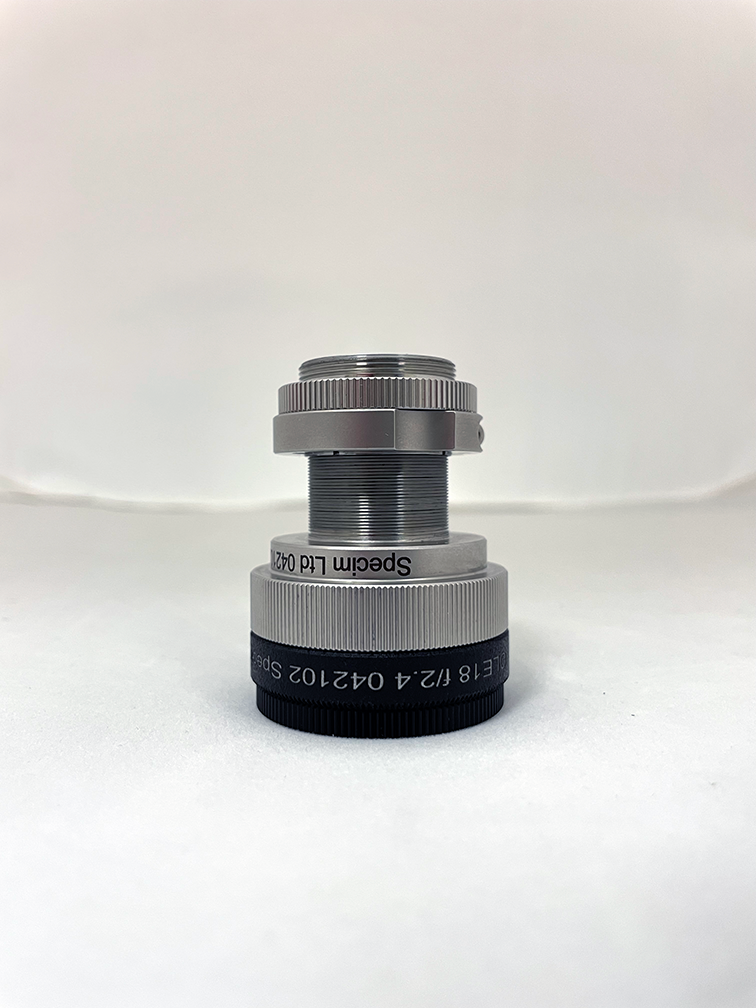
\includegraphics[width=1.94792in,height=\textheight]{images/specim-18.5.png}

}

\caption{Obiektyw 18.5 mm}

\end{figure}

\begin{figure}

{\centering 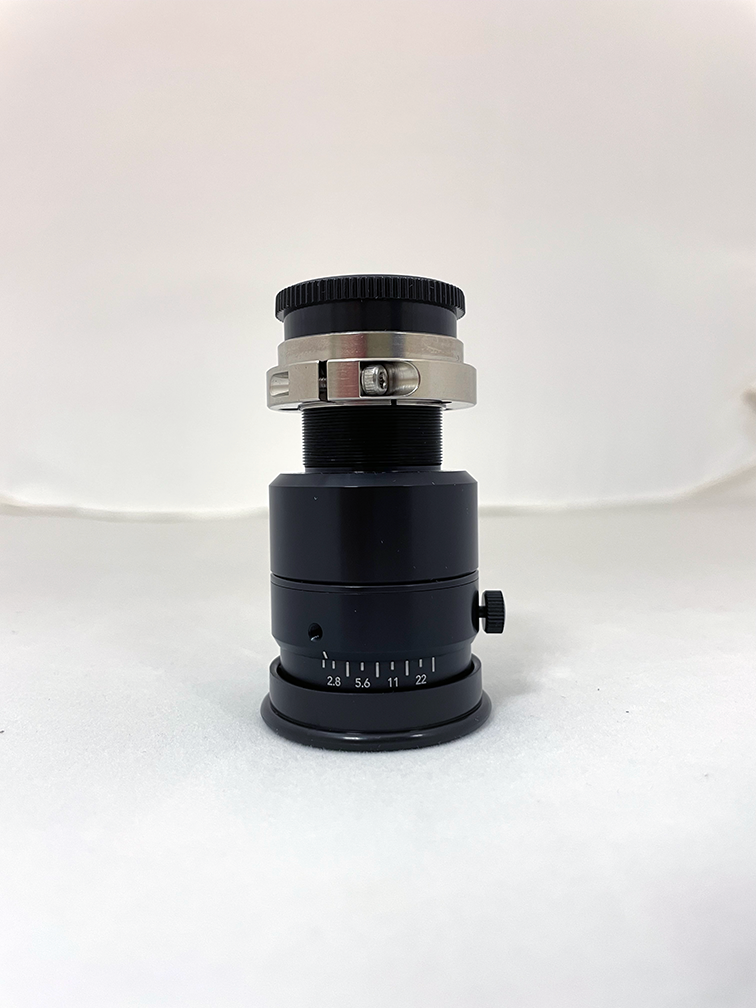
\includegraphics[width=1.94792in,height=\textheight]{images/specim-50.0.png}

}

\caption{Obiektyw 50.0 mm}

\end{figure}

\newpage{}

\hypertarget{zaux142ux105cznik-2-etykiety}{%
\section{Załącznik 2: etykiety}\label{zaux142ux105cznik-2-etykiety}}

\begin{figure}

{\centering 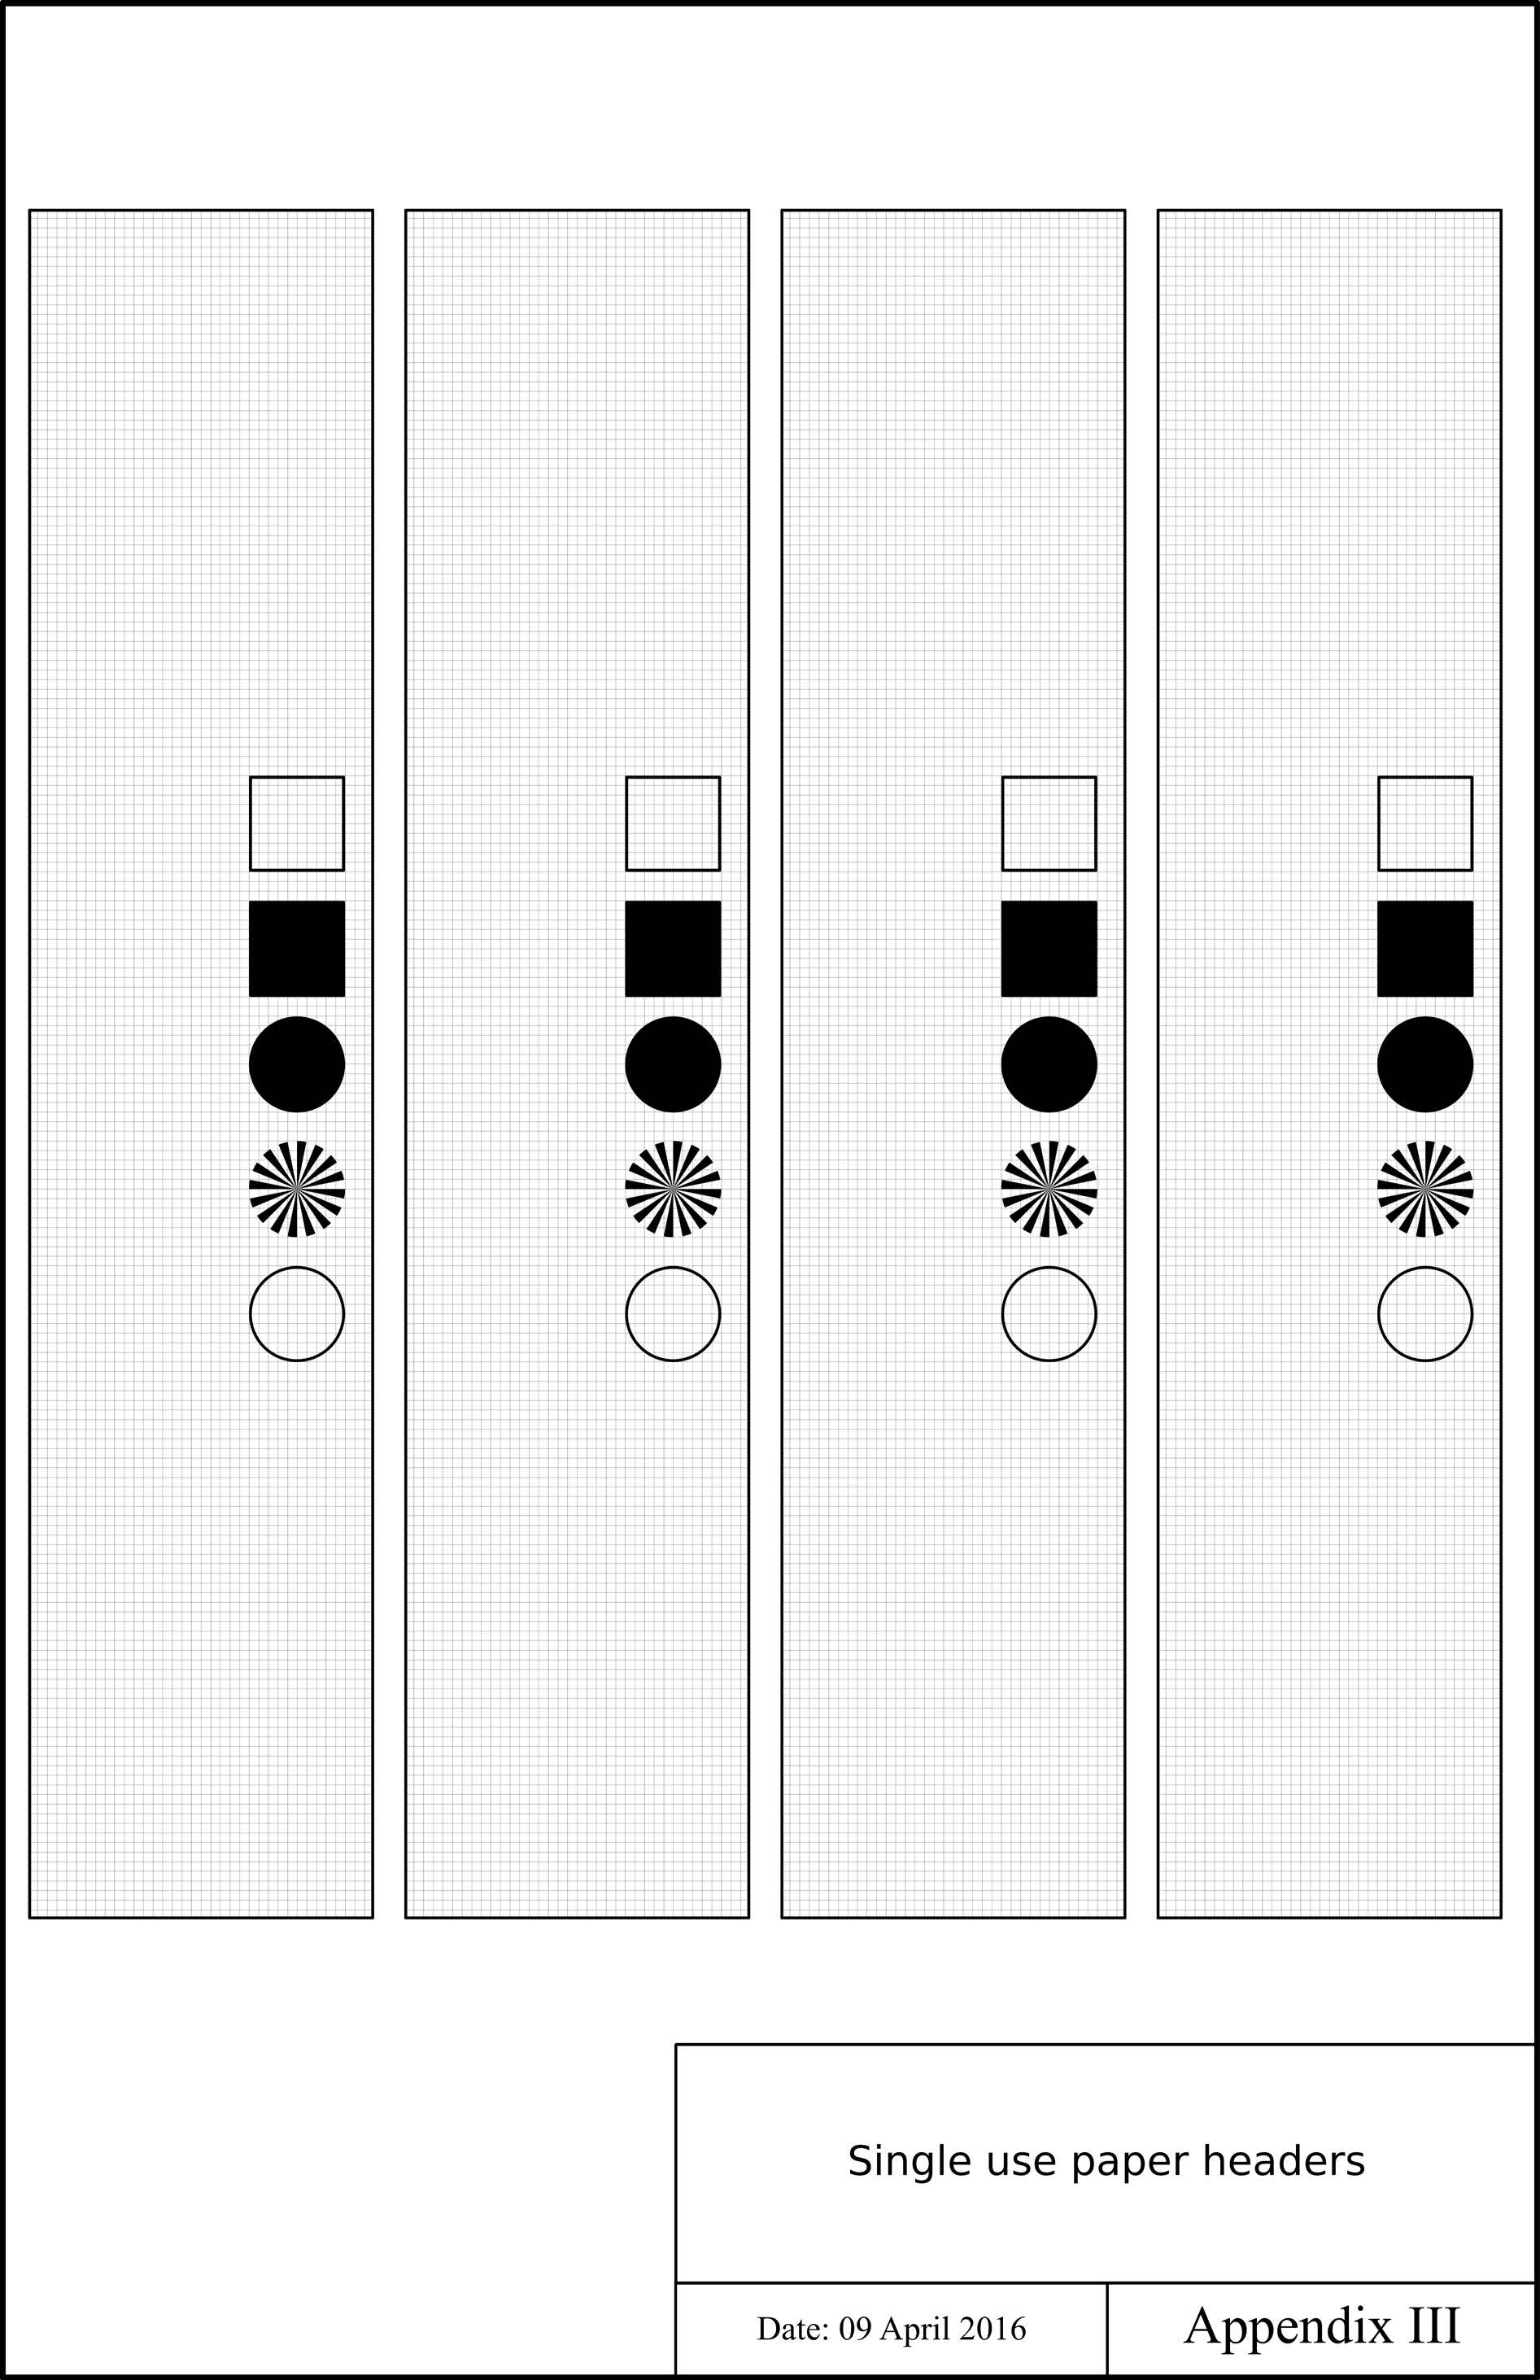
\includegraphics[width=0.5\textwidth,height=\textheight]{images/hsi_labels.jpg}

}

\caption{Wzór etykiet jednorazowych (źródło: Butz 2016)}

\end{figure}

\newpage{}

\hypertarget{rejestr-zmian-9}{%
\section{Rejestr zmian}\label{rejestr-zmian-9}}

\begin{itemize}
\tightlist
\item
  16.11.2022, MZ: wersja inicjalna.
\item
  17.11.2022, MZ: pierwsze poprawki.
\item
  30.11.2022, MZ: kolejne poprawki. Pierwsza wersja Quarto.
\item
  09.12.2022, MZ: poprawki, dodano info i wzór etykiet.
\item
  14.12.2022, MZ: poprawki, dodano informacje i fotografie obiektywów.
\end{itemize}

Maurycy Żarczyński

\hypertarget{okreux15blanie-zawartoux15bci-materii-organicznej-i-wux119glanuxf3w-metodux105-strat-na-praux17ceniu}{%
\chapter{Określanie zawartości materii organicznej i~węglanów metodą
strat na
prażeniu}\label{okreux15blanie-zawartoux15bci-materii-organicznej-i-wux119glanuxf3w-metodux105-strat-na-praux17ceniu}}

\begin{figure}

\href{https://geomorfologia.ug.edu.pl}{
\includegraphics[width=1.5625in,height=\textheight]{images/log-ug_pl.png}}

\end{figure}

Zakład Geomorfologii i Geologii Czwartorzędu --- PROCEDURA

\begin{center}\rule{0.5\linewidth}{0.5pt}\end{center}

\hypertarget{okreux15blenie-zawartoux15bci-materii-organicznej-loi550}{%
\section{\texorpdfstring{Określenie zawartości materii organicznej
(LOI\textsubscript{550})}{Określenie zawartości materii organicznej (LOI550)}}\label{okreux15blenie-zawartoux15bci-materii-organicznej-loi550}}

\begin{itemize}
\item
  Przygotować tygle porcelanowe (wymyć, wysuszyć i opisać odpowiednimi
  numerami).

  W laboratorium znajduje się specjalny pisak do porcelany, który
  pozostawia wyraźny napis po wypaleniu.
\item
  Zważyć tygle i zapisać masę w formularzu.
\item
  Przenieść do tygla określoną ilość suchego i homogenicznego osadu.

  Należy starać się zachować podobną masę próbek. Od \textbf{0.5 g} do
  \textbf{1.0 g}.
\item
  Zważyć tygle z suchym osadem i zapisać masę w formularzu.
\item
  Zaprogramować piec laboratoryjny na prażenie w temperaturze
  \textbf{550 °C} przez \textbf{4 godziny}.
\item
  Wstawić przygotowane próbki do pieca i uruchomić program.

  Po upłynięciu zadanego czasu piec automatycznie wyłączy się.
\item
  Uruchomić wentylator na czas prażenia.
\item
  Wystawić próbki z pieca (szczypcami) i wystudzić w eksykatorze do
  temperatury pokojowej.
\item
  Zważyć tygle i zapisać masę w formularzu.
\item
  Obliczyć zawartość materii organicznej (stratę na prażeniu)
  korzystając ze wzoru:

  \[
  LOI_{550} = (MS_{105} - MS_{550}) / MS_{105} × 100
  \]
\end{itemize}

gdzie:

\textbf{LOI\textsubscript{550}}: strata na prażeniu utożsamiana z
zawartością materii organicznej (\%);

\textbf{MS\textsubscript{105}}: masa osadu wysuszonego w 105 °C (g);

\textbf{MS\textsubscript{550}}: masa osadu wyprażonego w 550 °C (g).

\hypertarget{okreux15blenie-zawartoux15bci-wux119glanuxf3w-loi950}{%
\section{\texorpdfstring{Określenie zawartości węglanów
(LOI\textsubscript{950})}{Określenie zawartości węglanów (LOI950)}}\label{okreux15blenie-zawartoux15bci-wux119glanuxf3w-loi950}}

\begin{itemize}
\item
  Upewnić się, że oznaczenia tygli są wyraźne. Poprawić jeśli to
  konieczne.
\item
  Zaprogramować piec laboratoryjny na prażenie w temperaturze
  \textbf{950 °C} przez \textbf{2 godziny}.
\item
  Wstawić zważone po wyprażeniu w temperaturze \textbf{550 °C} próbki
  ponownie do pieca i uruchomić program.

  Po upłynięciu zadanego czasu piec automatycznie wyłączy się.
\item
  Uruchomić wentylator na czas prażenia.
\item
  Wystawić próbki z pieca (szczypcami) i wystudzić w eksykatorze do
  temperatury pokojowej.
\item
  Zważyć tygle i zapisać masę w formularzu.
\item
  Przenieść próbki do opisanych pojemników i szczelnie zamknąć lub
  postępować zgodnie z dalszymi procedurami.
\item
  Obliczyć zawartość węglanów (stratę na prażeniu) korzystając ze wzoru:

  \[
  LOI_{950} = (MS_{550} - MS_{950}) / MS_{105} × 100 × 1.36
  \]
\end{itemize}

gdzie:

\textbf{LOI\textsubscript{950}}: strata na prażeniu utożsamiana z
zawartością węglanów (\%);

\textbf{MS\textsubscript{550}}: masa osadu wyprażonego w 550 °C (g);

\textbf{MS\textsubscript{950}}: masa osadu wyprażonego w 950 °C (g);

\textbf{1.36}: przelicznik wynikający ze stosunku masy molowej
\(CO_3^{2-}:CO_2\).

\hypertarget{rejestr-zmian-10}{%
\section{Rejestr zmian}\label{rejestr-zmian-10}}

01.12.2022, MZ -- wersja inicjalna Quarto. Rozwinięcie treści.

Karolina Molisak, Maurycy Żarczyński \texttt{r\ Sys.Date()}

\hypertarget{okreux15blanie-zawartoux15bci-materii-mineralnej}{%
\chapter{Określanie zawartości materii
mineralnej}\label{okreux15blanie-zawartoux15bci-materii-mineralnej}}

\begin{figure}

\href{https://geomorfologia.ug.edu.pl}{
\includegraphics[width=1.5625in,height=\textheight]{images/log-ug_pl.png}}

\end{figure}

Zakład Geomorfologii i Geologii Czwartorzędu --- PROCEDURA

\begin{center}\rule{0.5\linewidth}{0.5pt}\end{center}

\hypertarget{praux17cenie-w-piecu-muflowym}{%
\section{Prażenie w piecu
muflowym}\label{praux17cenie-w-piecu-muflowym}}

\begin{itemize}
\item
  Przygotować tygle porcelanowe (wymyć, wysuszyć i opisać odpowiednimi
  numerami).

  W laboratorium znajduje się specjalny pisak do porcelany, który
  pozostawia wyraźny napis po wypaleniu.
\item
  Zważyć tygle i zapisać masę w formularzu.
\item
  Przenieść do tygla określoną ilość suchego i homogenicznego osadu.

  Należy starać się zachować podobną masę próbek. Około \textbf{0.2 g}.
\item
  Zważyć tygle z suchym osadem i zapisać masę w formularzu.
\item
  Zaprogramować piec laboratoryjny na prażenie w temperaturze
  \textbf{550 °C} przez \textbf{4 godziny}.
\end{itemize}

\begin{itemize}
\item
  Wstawić przygotowane próbki do pieca i uruchomić program.

  Po upłynięciu zadanego czasu piec automatycznie wyłączy się.
\item
  Uruchomić wentylator na czas prażenia.
\item
  Wystawić próbki z pieca (szczypcami) i wystudzić w eksykatorze do
  temperatury pokojowej.
\item
  Zważyć tygle i zapisać masę w formularzu.
\item
  Upewnić się, że oznaczenia tygli są wyraźne. Poprawić jeśli to
  konieczne.
\item
  Zaprogramować piec laboratoryjny na prażenie w temperaturze
  \textbf{950 °C} przez \textbf{2 godziny}.
\item
  Wstawić zważone po wyprażeniu w temperaturze 550 °C próbki ponownie do
  pieca i uruchomić program.

  Po upłynięciu zadanego czasu piec automatycznie wyłączy się.
\item
  Uruchomić wentylator na czas prażenia.
\item
  Wystawić próbki z pieca (szczypcami) i wystudzić w eksykatorze do
  temperatury pokojowej.
\item
  Zważyć tygle i zapisać masę w formularzu.
\end{itemize}

\hypertarget{mineralizacja}{%
\section{Mineralizacja}\label{mineralizacja}}

\begin{itemize}
\item
  Przenieść wyprażony osad do zlewek \textbf{250 ml} i zalać \textbf{100
  ml 2 mol NaOH}.
\item
  Wymieszać roztwór i przykryć zlewki.
\item
  Nastawić płytę grzejną na temperaturę \textbf{200 °C}.
\item
  Podgrzać roztwór w zlewkach do około \textbf{100 °C} (aż zacznie lekko
  wrzeć).
\item
  Wrzucić mieszadło i ustawić zlewkę na mieszadle magnetycznym na
  \textbf{6 h} w maksymalnej temperaturze.

  Zlewki należy co jakiś czas ręcznie wymieszać, żeby osad nie
  przyklejał się do ścianek.
\item
  Po zakończeniu mieszania wyciągnąć mieszadła magnetyczne, spłukując je
  wodą dejonizowaną.
\item
  Zlewki pozostawić na noc do wystygnięcia i osadzenia się osadu na~dnie
  zlewki.
\item
  Następnego dnia usunąc jak najwięcej cieczy (\emph{supernatantu}) za
  pomocą pipety.

  Uważać, żeby nie zaciągnąć osadu.
\item
  Pod digestorium: pozostałą zawartość zlewek przesączyć na lejku przez
  sączek ilościowy. Przepłukać zlewkę i sączek kilkukrotnie \textbf{HCl
  10 \%}.
\item
  Na koniec dokładnie spłukać zlewkę wodą destylowaną w celu całkowitego
  wypłukania osadu (w~szczególności materii mineralnej).
\item
  Przygotować tygle porcelanowe (wymyć, wysuszyć i opisać odpowiednimi
  numerami).

  W laboratorium znajduje się specjalny pisak do porcelany, który
  pozostawia wyraźny napis po wypaleniu.
\item
  Zważyć tygle i zapisać masę w formularzu.
\item
  Umieścić sączki w tyglach.
\end{itemize}

\begin{itemize}
\tightlist
\item
  Zaprogramować piec laboratoryjny na prażenie w temperaturze
  \textbf{550 °C przez 4 godziny}.
\end{itemize}

\begin{itemize}
\item
  Wstawić przygotowane próbki do pieca i uruchomić program.

  Po upłynięciu zadanego czasu piec automatycznie wyłączy się.
\item
  Uruchomić wentylator na czas prażenia.
\item
  Wystawić próbki z pieca (szczypcami) i wystudzić w eksykatorze do
  temperatury pokojowej.
\item
  Zważyć tygle i zapisać masę w formularzu.\newpage{}
\end{itemize}

\hypertarget{rejestr-zmian-11}{%
\section{Rejestr zmian}\label{rejestr-zmian-11}}

01.12.2022, MZ -- wersja inicjalna Quarto. Rozwinięcie treści. M
zamienione na mol zgodnie z wytycznymi SI.

Anna Poraj-Górska, Karolina Molisak, Maurycy Żarczyński
\texttt{r\ Sys.Date()}

\hypertarget{analiza-zawartoux15bci-azotu-i-fosforu-caux142kowitego}{%
\chapter{Analiza zawartości azotu i fosforu
całkowitego}\label{analiza-zawartoux15bci-azotu-i-fosforu-caux142kowitego}}

\begin{figure}

\href{https://geomorfologia.ug.edu.pl}{
\includegraphics[width=1.5625in,height=\textheight]{images/log-ug_pl.png}}

\end{figure}

Zakład Geomorfologii i Geologii Czwartorzędu --- PROCEDURA

\begin{center}\rule{0.5\linewidth}{0.5pt}\end{center}

\hypertarget{przygotowanie-pruxf3bek}{%
\section{Przygotowanie próbek}\label{przygotowanie-pruxf3bek}}

\begin{itemize}
\item
  Przygotować odkręcane probówki. Po jednej na azot oraz fosfor.
\item
  Próbki wody dokładnie wymieszać.
\item
  Odmierzyć po 10 ml próbki na każdą z analiz.
\item
  Przygotować termoreaktor.
\end{itemize}

\hypertarget{fosfor-caux142kowity-ptot}{%
\section{\texorpdfstring{Fosfor całkowity
(P\textsubscript{tot})}{Fosfor całkowity (Ptot)}}\label{fosfor-caux142kowity-ptot}}

\hypertarget{wstux119pne-przygotowanie-crackset10}{%
\subsection{Wstępne przygotowanie:
CrackSet10}\label{wstux119pne-przygotowanie-crackset10}}

\begin{itemize}
\item
  Do próbki dodać 1 kroplę odczynnika \textbf{R-1}, wymieszać.
\item
  Dodać porcję odczynnika \textbf{R-2}, wymieszać.
\item
  Próbki należy ogrzewać w termoreaktorze w temperaturze 120 °C przez 1
  godzinę.
\item
  Odstawić próbki do chłodni na około 15 minut w celu ostudzenia.
\item
  Po ochłodzeniu dodać 3 krople odczynnika \textbf{R-3}, wymieszać.
\item
  Sprawdzić pH, wymagane 3 lub wyższe.
\end{itemize}

\hypertarget{oznaczanie-zawartoux15bci-fosforu-caux142kowitego}{%
\subsection{Oznaczanie zawartości fosforu
całkowitego}\label{oznaczanie-zawartoux15bci-fosforu-caux142kowitego}}

\begin{itemize}
\item
  Do wstępnie przygotowanej próbki dodać 10 kropli odczynnika
  \textbf{P-1A}, wymieszać.
\item
  Dodać 2 mikrołyżeczki odczynnika \textbf{P-2A}, zamknąć szczelnie,
  mieszać energicznie do całkowitego rozpuszczenia się odczynnika.
\item
  Odstawić na 5 minut, czas zajścia reakcji.
\item
  Przelać próbkę do kuwety \textbf{50 mm}.
\item
  Wykonać pomiar zadając metodę poprzez umieszczenie kodu kreskowego w
  spektrofotometrze.
\end{itemize}

\hypertarget{azot-caux142kowity-ntot}{%
\section{\texorpdfstring{Azot całkowity
(N\textsubscript{tot})}{Azot całkowity (Ntot)}}\label{azot-caux142kowity-ntot}}

\hypertarget{wstux119pne-przygotowanie-crackset20}{%
\subsection{Wstępne przygotowanie:
CrackSet20}\label{wstux119pne-przygotowanie-crackset20}}

\begin{itemize}
\item
  Do próbki dodać 1 łyżeczkę (niebieską) odczynnika \textbf{R-1},
  rozpuścić.
\item
  Dodać 6 kropli odczynnika \textbf{R-2}, zakręcić i wymieszać.
\item
  Próbki należy ogrzewać w termoreaktorze w temperaturze 120 °C przez 1
  godzinę.
\item
  Odstawić próbki do chłodni na około 15 minut w celu ostudzenia.
\end{itemize}

\hypertarget{oznaczanie-zawartoux15bci-azotu-caux142kowitego}{%
\subsection{Oznaczanie zawartości azotu
całkowitego}\label{oznaczanie-zawartoux15bci-azotu-caux142kowitego}}

\begin{itemize}
\item
  Przygotować puste próbówki.
\item
  W próbówce umieścić odczynnik \textbf{NO3-1A} (pierwszy poziom
  niebieskiej mikrołyżeczki).
\item
  Dodać 5 ml odczynnika \textbf{NO3-2A}. Mieszać do momentu
  rozpuszczenia się odczynnika \textbf{NO3-1A}.
\item
  Dodać 1.5 ml wstępnie przygotowanej próbki do odczynnika wlewając
  pipetą po ściankach przechylonej próbówki. Po dodaniu próbki
  \textbf{natychmiast} intensywnie wymieszać trzymając probówkę za górną
  jej część ponieważ próbka w trakcie reakcji zrobi się \textbf{gorąca}.

  W trakcie tych czynność użytkownik powinien mieć nałożone rękawice i
  okulary ochronne.
\item
  Odstawić gorący roztwór na 10 minut, czas zajścia reakcji. \textbf{Nie
  chłodzić zimną wodą}.
\item
  Przelać próbkę do kuwety \textbf{10 mm}.
\item
  Wykonać pomiar zadając metodę poprzez umieszczenie kodu kreskowego w
  spektrofotometrze.
\end{itemize}

\hypertarget{rejestr-zmian-12}{%
\section{Rejestr zmian}\label{rejestr-zmian-12}}

01.12.2022, MZ -- wersja inicjalna Quarto. Rozwinięcie treści.

Karolina Molisak, Maurycy Żarczyński \texttt{r\ Sys.Date()}

\hypertarget{przygotowywanie-pruxf3b-do-oznaczania-aktywnoux15bci-210pb}{%
\chapter{\texorpdfstring{Przygotowywanie prób do oznaczania aktywności
\textsuperscript{210}Pb}{Przygotowywanie prób do oznaczania aktywności 210Pb}}\label{przygotowywanie-pruxf3b-do-oznaczania-aktywnoux15bci-210pb}}

\begin{figure}

\href{https://geomorfologia.ug.edu.pl}{
\includegraphics[width=1.5625in,height=\textheight]{images/log-ug_pl.png}}

\end{figure}

Zakład Geomorfologii i Geologii Czwartorzędu --- PROCEDURA

\begin{center}\rule{0.5\linewidth}{0.5pt}\end{center}

\hypertarget{etap-i}{%
\section{Etap I}\label{etap-i}}

\begin{itemize}
\item
  Przygotować zestaw pojemników do odważenia i do mineralizacji (wymyć i
  wysuszyć).
\item
  Postawić pojemnik do odważania na wadze analitycznej, wytarować,
  umieścić w pojemniku około \textbf{0.2 g} suchego osadu i zapisać jego
  masę.
\item
  Przesypać osad do pojemnika teflonowego do mineralizacji.
\item
  Pobrać \textbf{3 cm\textsuperscript{3}} stężonego
  \textbf{HNO\textsubscript{3} (65 \%)}, przenieść do pojemnika
  jednocześnie spłukując ścianki, a~następnie przelać do pojemnika
  teflonowego.
\item
  Pobrać pipetą \textbf{200 µl} roztworu wzorcowego
  \textsuperscript{\textbf{209}}\textbf{Po} i przenieść do pojemnika
  teflonowego.
\item
  Nałożyć korki na pojemniki teflonowe i szczelnie zakręcić. Delikatnie
  wymieszać i wstawić do mineralizatora, po czym włączyć program
  (Classical Methods) \texttt{Pb-210\ HNO3} (100 °C przez 2 h).
\item
  Wystawić pojemniki z mineralizatora, odkręcić ostrożnie (pod
  dygestorium) i dodać \textbf{3 cm\textsuperscript{3}} stężonego
  \textbf{HClO\textsubscript{4} (70 \%)}.
\item
  Zakręcić szczelnie pojemniki teflonowe, wstawić do mineralizatora i
  włączyć program \texttt{Pb-210\ HClO4} (100 °C przez 2 h).
\item
  Wystawić pojemniki teflonowe z mineralizatora, odkręcić ostrożnie i
  dodać \textbf{3 cm\textsuperscript{3}} stężonego \textbf{HF (40 \%)}.
\item
  Zakręcić szczelnie pojemniki teflonowe, wstawić do mineralizatora i
  włączyć program \texttt{Pb-210\ HF} (100 °C przez 4 h).
\end{itemize}

\hypertarget{etap-ii}{%
\section{Etap II}\label{etap-ii}}

\begin{itemize}
\item
  Wystawić pojemniki teflonowe z mineralizatora i przenieść za pomocą
  \textbf{6 mol HCl (5 cm\textsuperscript{3})} roztwór i~pozostałość
  osadu ilościowo do parowniczek teflonowych (wymieszać osad w
  pojemnikach teflonowych, przelać do parowniczki, wypłukać pojemnik
  teflonowy \textbf{HCl} i przelać do parowniczki).
\item
  Odparować na płycie grzejnej (\textbf{200 °C}, płytę zabezpieczyć
  folią aluminiową) bez przykrycia do pojawienia się wyraźnie białych
  dymów, następnie przykryć pokrywką teflonową i ogrzewać dalej pod
  przykryciem \textbf{min. 30 minut}, aż do sklarowania roztworu
  (\textbf{max. 1 h}).
\item
  Odkryć i dodać \textbf{3 cm\textsuperscript{3} 6 mol HCl}, następnie
  odparować do suchej pozostałości.

  \textbf{Nie prażyć}.
\item
  Rozpuścić suchą pozostałość w \textbf{27 cm\textsuperscript{3} 0.5 mol
  HCl}, dodać ok. \textbf{0.1 g kwasu askorbinowego} i~\textbf{0.1 g
  hydroksyloaminy}.
\item
  Podgrzać roztwór do temperatury \textbf{90 °C}. W międzyczasie opisać
  blaszki srebrne symbolami prób oraz datą i zamontować w uchwytach
  (czystą częścią do góry).
\item
  Wrzucić magnesy i zamknąć naczynia do depozycji. Ustawić naczynia na
  mieszadle magnetycznym, ustawić podgrzewanie na wartość \textbf{10}
  (maksimum) i obroty na wartość \textbf{1}.

  Proces depozycji powinien trwać co najmniej \textbf{4 h}.
\item
  Wyciągnąć blaszki srebrne, spłukać wodą dejonizowaną, przetrzeć
  \textbf{metanolem} lub \textbf{etanolem}, sprawdzić podpisy i
  zabezpieczyć.
\end{itemize}

\hypertarget{rejestr-zmian-13}{%
\section{Rejestr zmian}\label{rejestr-zmian-13}}

01.12.2022, MZ -- wersja inicjalna Quarto. Rozwinięcie treści. M
zamienione na mol zgodnie z wytycznymi SI.

Wojciech Tylmann, Karolina Molisak, Joanna Piłczyńska, Maurycy
Żarczyński \texttt{r\ Sys.Date()}

\hypertarget{ekstrakcja-pigmentuxf3w-z-osaduxf3w-jeziornych}{%
\chapter{Ekstrakcja pigmentów z osadów
jeziornych}\label{ekstrakcja-pigmentuxf3w-z-osaduxf3w-jeziornych}}

\begin{figure}

\href{https://geomorfologia.ug.edu.pl}{
\includegraphics[width=1.5625in,height=\textheight]{images/log-ug_pl.png}}

\end{figure}

Zakład Geomorfologii i Geologii Czwartorzędu --- PROCEDURA

\begin{center}\rule{0.5\linewidth}{0.5pt}\end{center}

\hypertarget{materiaux142y-eksploatacyjne-i-urzux105dzenia-1}{%
\section{Materiały eksploatacyjne i
urządzenia}\label{materiaux142y-eksploatacyjne-i-urzux105dzenia-1}}

\hypertarget{odczynniki-chemiczne-1} (klasa czystości \textbf{HPLC}): rozpuszczalnik.
\item
  Aceton \textbf{techniczny}: czyszczenie naczyń i urządzeń.
\item
  Woda \textbf{redestylowana (\emph{MilliQ})}.
\item
  Azot techniczny.
\item
  Neodisher Laboclean.

  Neodisher LaboClean FLA: płynny, wysoko-alkaliczny środek o wysokim
  działaniu dyspergującym.
\end{itemize}

\hypertarget{urzux105dzenia-1}{%
\subsection{Urządzenia}\label{urzux105dzenia-1}}

\begin{itemize}
\item
  Wyciąg laboratoryjny.

  Stężony aceton (C\textsubscript{3}H\textsubscript{6}O) to
  rozpuszczalnik organiczny, który wymaga pracy pod włączonym
  \textbf{wyciągiem laboratoryjnym}. Aceton jest wysoce
  \textbf{łatwopalny}. Aceton ma silne działanie \textbf{drażniące}.
\item
  Myjka ultradźwiękowa.
\item
  Wirówka laboratoryjna.
\item
  Wytrząsarka typu \emph{Vortex}.
\item
  Piec laboratoryjny do wypiekania szkła laboratoryjnego.
\item
  Suszarka laboratoryjna.
\item
  Liofilizator.
\item
  Szklane cylindry wolumetryczne:

  \begin{itemize}
  \item
    \textbf{500 ml}.
  \item
    \textbf{1000 ml}.
  \end{itemize}
\item
  Szklane zlewki do pipetowania acetonu.
\item
  Pipeta do acetonu \textbf{1000 µL} i końcówki (odpowiednie do
  acetonu).
\item
  Blok grzewczy.
\item
  Ewaporator (parownik azotowy) N\textsubscript{2}.

  \begin{itemize}
  \item
    Igły do ewaporatora N\textsubscript{2}.
  \item
    Metalowy statyw na próbki w brązowych fiolkach.
  \end{itemize}

  Np. urządzenie \emph{Turbovap}.
\item
  Statywy na próbki.
\item
  Waga analityczna i urządzenie antystatyczne, mikrołyżeczka.
\item
  Łaźnia lodowa.

  Taca wypełniona wkładami chłodzącymi.
\end{itemize}

\hypertarget{pozostaux142e-1}{%
\subsection{Pozostałe}\label{pozostaux142e-1}}

\begin{itemize}
\item
  Falkony polipropylenowe (PP) \textbf{25 ml} lub \textbf{50 ml}
  Corning™.

  Zwykły plastik reaguje ze stężonym acetonem.\\
  Jednorazowe.
\item
  Fiolki z brązowego szkła z zakrętkami \textbf{25 ml} lub \textbf{50
  ml}.

  Etykiety przyklejone taśmą.
\item
  Folia aluminiowa.
\item
  Długie, szklane pipety Pasteura.

  Jednorazowe.
\item
  Smoczek silikonowy do pipet.
\end{itemize}

\hypertarget{czyszczenie-1}{%
\section{Czyszczenie}\label{czyszczenie-1}}

Szkło laboratoryjne musi zostać wypieczone w piecu (\textbf{500 °C},
\textbf{12 h}) lub wyczyszczone acetonem (\textbf{5 razy}).

\hypertarget{fiolki-brux105zowe}{%
\subsection{Fiolki brązowe}\label{fiolki-brux105zowe}}

\begin{itemize}
\item
  Namaczać przez kilka godzin w wodzie z dodatkiem Neodisher Laboclean.
\item
  Umyć w zmywarce laboratoryjnej.

  Program do mycia szkła i Neodisher Laboclean.
\item
  Wysuszyć w suszarce.
\item
  Zabezpieczyć folią aluminiową

  Uprzednio wyczyszczona acetonem lub wypalona.
\item
  Wypiec w piecu w temperaturze \textbf{500 °C}.

  Minimum \textbf{12 h}.
\end{itemize}

\hypertarget{zakrux119tki-do-fiolek-brux105zowych}{%
\subsection{Zakrętki do fiolek
brązowych}\label{zakrux119tki-do-fiolek-brux105zowych}}

\begin{itemize}
\item
  Przemyć wodą z kranu.
\item
  Umieścić w zlewce wypełnionej mieszanką \textbf{acetonu technicznego}
  i wody \textbf{redestylowanej (MilliQ)} w stosunku \textbf{1:1}.

  \begin{itemize}
  \tightlist
  \item
    Umieścić zlewkę w myjce ultradźwiękowej na \textbf{10 minut}.
  \end{itemize}
\item
  Umieścić w zlewce wypełnionej \textbf{acetonem technicznym}.

  \begin{itemize}
  \tightlist
  \item
    Umieścić zlewkę w myjce ultradźwiękowej na \textbf{10 minut}.
  \end{itemize}
\item
  Wysuszyć w suszarce.

  Odczynniki wykorzystane do mycia można wykorzystać ponownie, po
  zabezpieczeniu w szklanych butelkach.
\end{itemize}

\hypertarget{sec-igux142y-do-ewaporatora}{%
\subsection{Igły do ewaporatora}\label{sec-igux142y-do-ewaporatora}}

\begin{itemize}
\item
  Umieścić igły w zlewce wypełnionej acetonem technicznym.
\item
  Umieścić w myjce ultradźwiękowej na \textbf{3 × 10 minut}.
\end{itemize}

\hypertarget{utylizacja}{%
\subsection{Utylizacja}\label{utylizacja}}

\begin{itemize}
\item
  Aceton zgodnie z wymogami.
\item
  Falkony i szklane pipety Pasteura muszą zostać dokładnie umyte i
  wyrzucone do recyclingu.
\end{itemize}

\hypertarget{przygotowanie-osaduxf3w-1}{%
\section{Przygotowanie osadów}\label{przygotowanie-osaduxf3w-1}}

\begin{itemize}
\item
  Próbki wysuszyć w liofilizatorze.

  Wysoka temperatura przy suszeniu w suszarce prowadzi do degradacji
  pigmentów.\\
  Jeśli ekstrakcja wykonana zostanie w ciągu tygodnia, próbki można
  przechowywać w eksykatorze. Dłuższej przechowywanie wymaga zamrożenia
  próbek i ich ponownego dosuszenia.
\item
  Na osobnej części osadów dokonać analizy metodą strat na prażeniu
  \textbf{550 °C}.

  Laboratorium PRL: obliczenie koncentracji materii organicznej na
  podstawie wyników \textbf{CNS}.
\item
  Naważyć \textbf{0.5 g} zhomogenizowanego osadu do falkonów
  polipropylenowych (PP) \textbf{25 ml}.

  Czyścić narzędzia acetonem technicznym, korzystać z urządzenia
  antystatycznego.\\
  W szczególnych przypadkach masa osadu może wynosić poniżej
  \textbf{0.50 g}, nie mniej niż \textbf{0.25 g}.\\
  Przy wysokiej zawartości OM \textbf{0.25 g} do \textbf{0.50 g}, w
  przypadku osadów klastycznych \textbf{1.00 g}.
\item
  Oznaczyć falkon oraz nakrętkę symbolem próbki.
\end{itemize}

\hypertarget{ekstrakcja-pigmentuxf3w}{%
\section{Ekstrakcja pigmentów}\label{ekstrakcja-pigmentuxf3w}}

\begin{itemize}
\item
  Przygotować stanowisko pracy, przykryć powierzchnie pod wyciągiem
  laboratoryjnym folią aluminiową, która uprzednio została wyczyszczona
  acetonem.
\item
  W miarę możliwości wyłączyć zbędne oświetlenie.
\item
  Przykrywać próbki folią aluminiową.
\item
  Wypełnić zlewkę szklaną acetonem 100\%.

  Nie pipetować bezpośrednio z butelki.
\item
  Nabrać acetonu do pipety w celu wypłukania.

  Zużyty aceton pipetować do osobnej zlewki.
\item
  Dodać 5 ml acetonu do falkona.

  Zwrócić uwagę na poprawne pipetowanie, w pipecie nie powinno być
  pęcherzyków powietrza.
\item
  Wymieszać na Vortexie przez \textbf{1 minutę}.
\item
  Umieścić w myjce ultradźwiękowej na \textbf{1 minutę}.
\item
  Odwirować.

  \begin{itemize}
  \item
    \textbf{10 minut}.
  \item
    \textbf{5000 rpm}.
  \end{itemize}

  Ten krok należy dostosować do możliwości wirówki. Niższe obroty
  wymagają dłuższego wirowania.
\item
  Sprawdzić czy supernatant jest czysty po odwirowaniu.

  Jeśli w rozpuszczalniku widoczna jest zawiesina należy powtórzyć
  wirowanie. Ciecz może być zabarwiona.
\item
  Usunąć supernatant z użyciem długiej szklanej pipety Pasteura i
  przenieść do brązowej fiolki.

  Fiolka musi mieć odpowiednią etykietę.\\
  Upewnić się, że cały supernatant został przeniesiony z falkona.
\item
  Powtórzyć ekstrakcję dwukrotnie z użyciem \textbf{5 ml} acetonu.
\item
  Odpowiednio oznaczone szklane pipety Pasteura pomiędzy cyklami
  przechowywać w szklanej zlewce.

  Każdej brązowej fiolce i falkonowi odpowiada jedna szklana pipeta
  Pasteura.
\item
  Brązowe fiolki pomiędzy etapami ekstrakcji zakryć przed światłem i
  przechowywać w łaźni lodowej.

  Jeśli supernatant \textbf{po trzecim cyklu} ekstrakcji nadal jest
  \textbf{wyraźnie zabarwiony} należy kontynuować ekstrakcję do
  osiągnięcia \textbf{czystego ekstraktu}.\\
  Istotne aby wszystkie próbki w danej serii przeszły \textbf{taki sam
  proces ekstrakcji}.\\
  Tak przygotowane ekstrakty można przechowywać w temperaturze
  \textbf{-20 °C} do okoła \textbf{1 miesiąca}. Wypełnienie probówki
  \textbf{N\textsubscript{2}} lub \textbf{Ar} i usunięcie
  \textbf{O\textsubscript{2}} pozytywnie wpływa na zachowanie pigmentów.
\end{itemize}

\hypertarget{koncentracja-i-rekonstytucja-roztworuxf3w}{%
\section{Koncentracja i rekonstytucja
roztworów}\label{koncentracja-i-rekonstytucja-roztworuxf3w}}

\hypertarget{odparowanie}{%
\subsection{Odparowanie}\label{odparowanie}}

\begin{itemize}
\item
  Ustawić blok grzewczy i ewaporator azotowy.
\item
  Z użyciem ewaporatora azotowego odparować próbki do suchej
  pozostałości.
\end{itemize}

Przed użyciem ewaporatora należy upewnić się, że igły zostały
wyczyszczone (Section~\ref{sec-igły-do-ewaporatora}).

\begin{itemize}
\item
  Umieścić próbki w brązowych fiolkach w bloku grzewczym pod
  ewaporatorem azotowym, ustawić temperaturę \textbf{35 °C}.
\item
  Otworzyć przepływ azotu.
\end{itemize}

Ciśnienie ustawić tak, aby zaobserwować niewielkie ugięcie powierzchni
roztworu.

\begin{itemize}
\tightlist
\item
  Odparowywać do uzyskania suchej pozostałości (około \textbf{4} do
  \textbf{6 godzin}).
\end{itemize}

\hypertarget{rekonstytucja}{%
\subsection{Rekonstytucja}\label{rekonstytucja}}

\begin{itemize}
\tightlist
\item
  Dodać \textbf{2 ml} acetonu do brązowej fiolki z wykorzystaniem pipety
  \textbf{1000 µl}.
\end{itemize}

Postępować bardzo precyzyjnie, upewnić się, że w pipecie nie ma
pęcherzyków powietrza.

\begin{itemize}
\item
  Zhomogenizować roztwór szklaną pipetą Pasteura.
\item
  Spłukać ścianki i w miarę możliwości odwirować na \emph{vortexie}.
\end{itemize}

Całość pigmentów musi się ponownie rozpuścić w acetonie. Może pojawić
się i pozostać biały nalot.

\hypertarget{filtrowanie}{%
\subsection{Filtrowanie}\label{filtrowanie}}

\hypertarget{pagebreak-rejestr-zmian-5}{%
\section{\texorpdfstring{\newpage{}Rejestr
zmian}{Rejestr zmian}}\label{pagebreak-rejestr-zmian-5}}

09.12.2022, MZ -- wersja inicjalna Quarto, procedura za: Andrea Sanchini
i Giulia Wienhues (Uniwersytet w~Bernie).

09.02.2023, MZ -- pełna wersja.

Maurycy Żarczyński \texttt{r\ Sys.Date()}

\hypertarget{pomiar-pigmentuxf3w-z-osaduxf3w-jeziornych-metoda-spektrofotometryczna}{%
\chapter{Pomiar pigmentów z osadów jeziornych: metoda
spektrofotometryczna}\label{pomiar-pigmentuxf3w-z-osaduxf3w-jeziornych-metoda-spektrofotometryczna}}

\begin{figure}

\href{https://geomorfologia.ug.edu.pl}{
\includegraphics[width=1.5625in,height=\textheight]{images/log-ug_pl.png}}

\end{figure}

Zakład Geomorfologii i Geologii Czwartorzędu --- PROCEDURA

\begin{center}\rule{0.5\linewidth}{0.5pt}\end{center}

\hypertarget{materiaux142y-eksploatacyjne-i-urzux105dzenia-2}{%
\section{Materiały eksploatacyjne i
urządzenia}\label{materiaux142y-eksploatacyjne-i-urzux105dzenia-2}}

\hypertarget{odczynniki-chemiczne-2} (klasa czystości \textbf{HPLC}): rozpuszczalnik.
\item
  Aceton \textbf{techniczny}: czyszczenie naczyń i urządzeń.
\item
  Woda \textbf{redestylowana (\emph{MilliQ})}.
\item
  Azot techniczny.
\item
  Neodisher Laboclean.

  Neodisher LaboClean FLA: płynny, wysoko-alkaliczny środek o wysokim
  działaniu dyspergującym.
\end{itemize}

\hypertarget{urzux105dzenia-2}{%
\subsection{Urządzenia}\label{urzux105dzenia-2}}

\begin{itemize}
\item
  Wyciąg laboratoryjny.

  Stężony aceton (C\textsubscript{3}H\textsubscript{6}O) to
  rozpuszczalnik organiczny, który wymaga pracy pod włączonym
  \textbf{wyciągiem laboratoryjnym}. Aceton jest wysoce
  \textbf{łatwopalny}. Aceton ma silne działanie \textbf{drażniące}.
\item
  Myjka ultradźwiękowa.
\item
  Wirówka laboratoryjna.
\item
  Wytrząsarka typu \emph{Vortex}.
\item
  Piec laboratoryjny do wypiekania szkła laboratoryjnego.
\item
  Suszarka laboratoryjna.
\item
  Szklane zlewki do pipetowania acetonu.
\item
  Pipeta do acetonu \textbf{100--1000 µl} i końcówki (odpowiednie do
  acetonu).
\item
  Pipeta do acetonu \textbf{50--250 µl} i końcówki (odpowiednie do
  acetonu).
\item
  Statywy na próbki.
\item
  Kolby wolumetryczne (cechowane).

  1 ml, 5 ml, 10 ml, 25 ml, 50 ml, 100 ml.
\end{itemize}

\hypertarget{pozostaux142e-2}{%
\subsection{Pozostałe}\label{pozostaux142e-2}}

\begin{itemize}
\item
  Mikrokuwety \textbf{400 µl} z zatyczkami.

  Kuwety łapać tylko za rogi. Upewnić się, że kuweta nie jest
  zanieczyszczona.
\item
  Długie, szklane pipety Pasteura.

  Jednorazowe.
\item
  Smoczek silikonowy do pipet.
\end{itemize}

\hypertarget{czyszczenie-2}{%
\section{Czyszczenie}\label{czyszczenie-2}}

\begin{itemize}
\item
  Wymyć ręcznie szkło laboratoryjne szczotką.
\item
  Umyć w zmywarce laboratoryjnej.

  Program do mycia szkła i Neodisher Laboclean.
\item
  Wypłukać wodą \textbf{redestylowaną (MilliQ)} i \textbf{Nanowater}
  \textbf{3 razy}.
\item
  Wyczyścić acetonem technicznym.
\item
  Zamknąć folią aluminiową, która uprzednio została wyczyszczona
  acetonem
\item
  Wypiec w piecu w temperaturze \textbf{292 °C}.
\end{itemize}

Minimum \textbf{12 h}.

\hypertarget{utylizacja-1}{%
\subsection{Utylizacja}\label{utylizacja-1}}

\begin{itemize}
\item
  Aceton zgodnie z wymogami.
\item
  Falkony i szklane pipety Pasteura muszą zostać dokładnie umyte i
  wyrzucone do recyclingu.
\end{itemize}

\hypertarget{przygotowanie-urzux105dzenia}{%
\section{Przygotowanie urządzenia}\label{przygotowanie-urzux105dzenia}}

\hypertarget{spektrofotometr}{%
\subsection{Spektrofotometr}\label{spektrofotometr}}

\begin{itemize}
\item
  Włączyć spektrofotometr i komputer.
\item
  Odczekać minimum \textbf{1 h} przed pomiarami.
\item
  Włączyć oprogramowanie \textbf{UVProbe}.
\item
  Wcisnąć F4 i kliknąć \texttt{Connect}.
\item
  Ustawić parametry:

  \begin{itemize}
  \item
    Zakres: \textbf{350} do \textbf{900 nm}.
  \item
    Żółty guzik ??.
  \item
    Method: spectrum.
  \item
    Scan speed: fast.
  \item
    Sampling interval: 0.1 nm.
  \item
    Scan mode: Single
  \item
    \texttt{Ok}.
  \end{itemize}
\end{itemize}

\hypertarget{pruxf3bki-ux15blepe-i-linia-bazowa}{%
\subsection{Próbki ślepe i linia
bazowa}\label{pruxf3bki-ux15blepe-i-linia-bazowa}}

\hypertarget{pruxf3bka-ux15blepa-blank},
  \textbf{HPLC}) do kuwety.
\end{itemize}

Sprawdzić czy próbka nie jest zanieczyszczona.\\
Upewnić się, że w końcówce pipety nie ma pęcherzyków powietrza.

\begin{itemize}
\tightlist
\item
  Zamknąć kuwetę zatyczką
\end{itemize}

Utrudnia odparowanie próbki oraz korozję urządzenia.

\begin{itemize}
\tightlist
\item
  Umieścić kuwetę w przedniej celi (cela pomiarowa).
\end{itemize}

Oznaczenie \emph{V} na kuwecie powinno znajdować się z boku.

\hypertarget{autozero-pruxf3bka-referencyjna},
  \textbf{HPLC}) do kuwety.
\end{itemize}

Sprawdzić czy próbka nie jest zanieczyszczona.\\
Upewnić się, że w końcówce pipety nie ma pęcherzyków powietrza.

\begin{itemize}
\tightlist
\item
  Zamknąć kuwetę zatyczką
\end{itemize}

Utrudnia odparowanie próbki oraz korozję urządzenia.

\begin{itemize}
\tightlist
\item
  Umieścić kuwetę w tylnej celi (cela referencyjna).
\end{itemize}

Oznaczenie \emph{V} na kuwecie powinno znajdować się z boku.

\begin{itemize}
\tightlist
\item
  Kliknąć \texttt{Baseline}
\end{itemize}

Po tym etapie wartość absorpcji powinna wskazywać zero.\\
Próbka referencyjna pozostaje w celi na czas wszystkich pomiarów.

\begin{itemize}
\tightlist
\item
  Wykonywać procedurę \emph{autozero} przed pomiarem nowego ekstraktu.
\end{itemize}

\hypertarget{pomiar-pruxf3bek}{%
\subsection{Pomiar próbek}\label{pomiar-pruxf3bek}}

\begin{itemize}
\tightlist
\item
  Ekstrakty są rozcieńczone tak, aby ogólna absorpcja mieściła się
  między \textbf{0.2} i \textbf{1.0 abs}.
\end{itemize}

W tym zakresie oznaczenie koncentracji ma charakter liniowy i nie wymaga
wykorzystania krzywych kalibracyjnych.

\hypertarget{rozcieux144czanie}{%
\subsubsection{Rozcieńczanie}\label{rozcieux144czanie}}

Do rozcieńczania ekstraktów można wykorzystać małą kolbę miarową lub
probówki Eppendorfa. Pozwala to na ponowy pomiar próbki przy wyższym
rozcieńczeniu po pipetowaniu bezpośrednio z kolby lub probówki.

\hypertarget{przykux142ad-110}{%
\paragraph{Przykład 1:10}\label{przykux142ad-110}}

\begin{itemize}
\item
  Wymieszać brązową fiolkę z ekstraktem na \emph{vortexie}.
\item
  Za pomocą pipety przenieść \textbf{2 × 250 µl} ekstraktu do
  \textbf{kolby 5 ml}.
\item
  Dodać aceton za pomocą szklanej pipety Pasteura do osiągnięcia
  \textbf{5 ml}.

  Uwaga: menisk jest \textbf{wklęsły}.
\item
  Wymieszać roztwór szklaną pipetą.
\end{itemize}

\hypertarget{pomiar-1}{%
\subsubsection{Pomiar}\label{pomiar-1}}

\begin{itemize}
\item
  Za pomocą pipety przenieść \textbf{400 µl} roztworu do kuwety.
\item
  Zamknąć kuwetę zatyczką.
\item
  Umieścić kuwetę w przedniej celi (cela pomiarowa).

  Oznaczenie \emph{V} na kuwecie powinno znajdować się z boku.
\item
  Kliknąć \texttt{Start}.
\end{itemize}

\hypertarget{zapis-i-eksport-danych}{%
\subsubsection{Zapis i eksport danych}\label{zapis-i-eksport-danych}}

Przy rozpoczęciu analizy pojawi się okno, w którym można wprowadzić
nazwę pliku. Jednak po zakończeniu analizy każdej z próbek
\textbf{trzeba zapisać plik ręcznie}. Inaczej dane zostaną utracone.

\hypertarget{zapis-danych}{%
\paragraph{Zapis danych}\label{zapis-danych}}

\texttt{File\ \textgreater{}\ Save\ as\ \textgreater{}\ nazwa\_pliku}

\hypertarget{eksport-danych}{%
\paragraph{Eksport danych}\label{eksport-danych}}

\texttt{Data\ Print}

Pojawi się tabela z danymi, które należy skopiować i wkleić do arkusza
kalkulacyjnego.

Należy \textbf{ręcznie} \textbf{rozszerzyć kolumny}, tak aby widoczne
były pełne nazwy. W innym wypadku dane nie skopiują się odpowiednio.

\hypertarget{ewaluacja-danych}{%
\paragraph{Ewaluacja danych}\label{ewaluacja-danych}}

Naturalne pigmenty to mieszanina barwników chlorofilowych i
karotenoidów, jednak spektrum uzyskane z próbki pozwala na ocenę tego,
jakie pigmenty są obecne w próbce.

Możliwe jest porównanie spektrum standardów z otrzymanymi w trakcie
analizy.

\hypertarget{przykux142ady}{%
\subparagraph{Przykłady}\label{przykux142ady}}

\begin{itemize}
\item
  Chl-a (absorption max. 430 and 663 nm)
\item
  Chl-b (absorption max. 463 and 648 nm)
\item
  Pheophytin-a (absorption max. 408 and 664nm)
\item
  Carotenoids (420--450 nm)
\item
  Bacteriochlorophyll-a (absorption max. 364 and 770 nm)

  \begin{itemize}
  \tightlist
  \item
    Bacteriopheophytin-a (absorption max. 357 and 746 nm)
  \end{itemize}
\item
  Bacteriochlorophyll-b (absorption max. 373 and 795 nm)

  \begin{itemize}
  \tightlist
  \item
    Bacteriopheophytin-b (absorption max. 367 and 776 nm)
  \end{itemize}
\item
  Bacteriochlorophyll-c, -d, -e (absorption max. 434, 427, 469 and 666,
  655, 654 nm)

  \begin{itemize}
  \tightlist
  \item
    Bacteriopheophytin-c, -d, -e (absorption max. 412, 406, 435 and 666,
    657, 665 nm)
  \end{itemize}
\end{itemize}

\hypertarget{obliczenia-fotometryczne}{%
\section{Obliczenia fotometryczne}\label{obliczenia-fotometryczne}}

\hypertarget{obliczenia-na-potrzeby-kalibracji-typu-proxy-proxy-dla-danych-hiperspektralnych.}{%
\subsection{Obliczenia na potrzeby kalibracji typu proxy-proxy dla
danych
hiperspektralnych.}\label{obliczenia-na-potrzeby-kalibracji-typu-proxy-proxy-dla-danych-hiperspektralnych.}}

\hypertarget{korekta-wartoux15bci-absorpcji}{%
\subsection{Korekta wartości
absorpcji}\label{korekta-wartoux15bci-absorpcji}}

Należy dokonać korekty wartości absorbcji jeśli absorbcja wynosi więcej
lub mniej niż \textbf{0} pomiędzy \textbf{720 nm} i \textbf{900 nm}.
Wartości przeskalować tak aby uzyskać \textbf{0} w zakresie \textbf{720}
nm i \textbf{900 nm}.

\begin{itemize}
\item
  Do określenia zawartości całkowitych karotenoidów i chloropigmentów,
  przy absencji bakteriochloropigmentów w próbce, można wykorzystać
  wartości absorbcji odpowiadające długości fali \textbf{750 nm}.
\item
  W przypadku obecności bakteriochloropigmentów w próbce, należy znaleźć
  odpowiednią wartość dla wybranej długości fali powyżej \textbf{750 nm}
  i wykorzystać do przeskalowania wyników.
\end{itemize}

Procedura opisana w artykule Sanchini i Grosjean (2020).

\hypertarget{obliczenia-caux142kowitych-chloropigmentuxf3w-a-oraz-bakteriofeofityny-a-ze-spektruxf3w-absorpcji}{%
\subsection{Obliczenia całkowitych chloropigmentów-a oraz
bakteriofeofityny-a ze spektrów
absorpcji}\label{obliczenia-caux142kowitych-chloropigmentuxf3w-a-oraz-bakteriofeofityny-a-ze-spektruxf3w-absorpcji}}

Koncentracje oblicza się z wykorzystaniem wzoru

\[
c = A_λ / (α_λ × l)
\]

gdzie:

\textbf{l}: szerokość kuwety (cm);

\textbf{A\textsubscript{λ}}: zmierzona absorbcja odpowiadająca wybranej
długości fali;

\textbf{α\textsubscript{λ}}: molowy współczynnik ekstynkcji wynoszący
\textbf{88.77 × 10\textsuperscript{-3} × L × cm\textsuperscript{-1} ×
mg\textsuperscript{-1}} dla chloropigmentów-a przy długości fali
\textbf{666 nm} (Jeffrey and Humphrey, 1975) oraz \textbf{52.855 ×
10\textsuperscript{-3} × L × cm\textsuperscript{-1} ×
mg\textsuperscript{-1}} dla bakteriofeofityny-a przy długości fali
\textbf{750 nm} (Fiedor et al., 2002).

Wynik to koncentracja zmierzona w kuwecie (\textbf{mg/l}), który należy
skorygować odpowiednio do rozcieńczenia oraz wagi próbki.

Przykładowe obliczenia zebrane zostały w arkuszu
\texttt{Spectrophotometer\_calculator.xlsx}

\[
(absorbcja piku) / k × (wspóczynnik rozcieńczenia) × (waga próbki) / (obejętość ektraktu)
\]

gdzie:

\textbf{k}: stała, \textbf{0.080770} dla chloropigmentów przy piku o
długości fali \textbf{666 nm} (Jeffrey and Humphrey, 1975) i
\textbf{0.052855} dla bakteriofeofityny przy piku dla długości fali
\textbf{750 nm} (Fiedor et al., 2002).

\hypertarget{obliczenia-choloroflu-a-b-i-c-ze-spektruxf3w-absorpcji}{%
\subsection{Obliczenia choloroflu a, b i c ze spektrów
absorpcji}\label{obliczenia-choloroflu-a-b-i-c-ze-spektruxf3w-absorpcji}}

\hypertarget{obliczenia-caux142kowitych-karotenoiduxf3w-ze-spektruxf3w-absorpcji}{%
\subsection{Obliczenia całkowitych karotenoidów ze spektrów
absorpcji}\label{obliczenia-caux142kowitych-karotenoiduxf3w-ze-spektruxf3w-absorpcji}}

\hypertarget{za-lichtenthaler-and-buschmann-2001}{%
\subsubsection{Za Lichtenthaler and Buschmann
(2001)}\label{za-lichtenthaler-and-buschmann-2001}}

W ekstrakcie materiału roślinnego zawierającym karotenoidy (\textbf{x +
c = xanatofile i karoteny}) w dodatku do chlorofili,
\textbf{A\textsubscript{470}} (region karotenoidów) oznacza się jako
sumę absorbcji dla chlorofilu-a, chlorofilu-b oraz karotenoidów:

\begin{itemize}
\tightlist
\item
  Aceton (czysty, 100\%):
\end{itemize}

\[
c_{(x + c)} = (1000 × A_{470} - 1.90_{C_a} – 63.14_{C_b}) / 214
\]

Aceton (20\% wody):

\[
c_{(x + c)} = (1000 × A_{470} - 1.82_{C_a} – 85.02_{C_b}) / 198
\]

gdzie:

\textbf{A\textsubscript{470}}: absorbcja dla długości fali \textbf{470
nm};

\textbf{C\textsubscript{a}}: xxx

\textbf{C\textsubscript{b}}: xxx

\hypertarget{za-guilizzoni-et-al.-2011-na-podstawie-zuxfcllig-et-al.-1981}_{1cm} × g_{LOI}
\]

gdzie:

\textbf{E\textsubscript{xxx}}: gęstość optyczna w kuwecie o ścieżce
optycznej \textbf{1 cm} (szerokość) dla długości fali \textbf{450 nm} i
\textbf{665 nm}, skorygowanych o gęstość optyczną dla długości fali
\textbf{750 nm};

\textbf{V}: objętość ekstraktu;

\textbf{E\textsuperscript{1\%}\textsubscript{1cm}}: średni współczynnik
ekstynkcji dla \textbf{1\%} roztworu ekstraktu z osadów (wagowo) dla
karotenoidów przy ścieżce optycznej (szerokość) \textbf{1 cm}. Równe
\textbf{2.250} (Züllig 1981; Leavitt and Hodgson 2001);

\textbf{E\textsubscript{450}}: główne pasmo absorbcji dla karotenoidów w
zakresie widzialnym;

\textbf{E\textsubscript{665}}: korekta na przybliżone pasmo absorbcji
chlorofili i pochodnych chlorofili odpowiadające długości fali
\textbf{665 nm};

\textbf{g\textsubscript{LOI}}: równoważnik strat na prażeniu dla mokrego
osadu, obliczony na podstawie zawartości osadów i suchej masy po LOI.

\hypertarget{funkcja-transferu-dla-fosforu-caux142kowitego}{%
\subsection{Funkcja transferu dla fosforu
całkowitego}\label{funkcja-transferu-dla-fosforu-caux142kowitego}}

\hypertarget{pagebreak-rejestr-zmian-6}{%
\section{\texorpdfstring{\newpage{}Rejestr
zmian}{Rejestr zmian}}\label{pagebreak-rejestr-zmian-6}}

09.12.2022, MZ -- wersja inicjalna Quarto, procedura za: Paul Zander,
Andrea Sanchini i Giulia Wienhues (Uniwersytet w~Bernie).

09.02.2023, MZ -- pełna wersja.

Maurycy Żarczyński \texttt{r\ Sys.Date()}

\hypertarget{ekstrakcja-sekwencyjna}{%
\chapter{Ekstrakcja sekwencyjna}\label{ekstrakcja-sekwencyjna}}

\begin{figure}

\href{https://geomorfologia.ug.edu.pl}{
\includegraphics[width=1.5625in,height=\textheight]{images/log-ug_pl.png}}

\end{figure}

Zakład Geomorfologii i Geologii Czwartorzędu --- PROCEDURA

\begin{center}\rule{0.5\linewidth}{0.5pt}\end{center}

\hypertarget{roztwory-ekstrahujux105ce}{%
\section{Roztwory ekstrahujące}\label{roztwory-ekstrahujux105ce}}

\textsc{Wszystkie odczynniki o czystości analitycznej (\emph{Ultrapure},
cz. d.~a.).}

\begin{itemize}
\item
  Roztwór \textbf{A}: \textbf{0.11 mol CH\textsubscript{3}COOH}

  \begin{quote}
  \textbf{25.0 cm\textsuperscript{3}} \textbf{lodowatego kwasu octowego
  (CH\textsubscript{3}COOH\textsubscript{bezw.})} dodać do \textbf{500.0
  cm\textsuperscript{3} wody redestylowanej (\emph{MilliQ})} i dopełnić
  do \textbf{1000.0 cm\textsuperscript{3}}, wymieszać (\textbf{C = 0.43
  mol/dm\textsuperscript{3}}). Następnie rozcieńczyć go czterokrotnie
  (\textbf{4}). Otrzymany roztwór o stężeniu \textbf{C = 0.11
  mol/dm\textsuperscript{3}} wykorzystać do ekstrakcji.
  \end{quote}
\item
  Roztwór \textbf{B}: \textbf{0.05 mol NH\textsubscript{2}OH·HCl}

  \begin{quote}
  Rozpuścić \textbf{6.95 g chlorowodorku hydroksyloaminy
  (NH\textsubscript{2}OH·HCl)} w \textbf{900.0 cm\textsuperscript{3}}
  \textbf{wody redestylowanej (\emph{MilliQ})} i zakwasić
  \textbf{stężonym kwasem azotowym (V)} do \textbf{pH = 2}. Dopełnić do
  \textbf{1000.0 cm\textsuperscript{3}} i wymieszać.
  \end{quote}
\item
  Roztwór \textbf{C}: \textbf{8.8 mol
  H\textsubscript{2}O\textsubscript{2} (30\%)}

  \begin{quote}
  Roztwór \textbf{H\textsubscript{2}O\textsubscript{2}} o stężeniu
  \textbf{8.8 mol/dm\textsuperscript{3}} (dostępny w handlu jako roztwór
  o stężeniu \textbf{30\%}).
  \end{quote}
\item
  Roztwór \textbf{D}: \textbf{1 mol
  CH\textsubscript{3}COONH\textsubscript{2}}

  \begin{quote}
  Rozpuścić \textbf{77.1 g octanu amonu
  (CH\textsubscript{3}COONH\textsubscript{4})} w \textbf{900.0
  cm\textsuperscript{3}} \textbf{wody redestylowanej (\emph{MilliQ})} i
  zakwasić \textbf{stężonym kwasem azotowym (V)} do \textbf{pH = 2}.
  Dopełnić do \textbf{1000.0 cm\textsuperscript{3}} i wymieszać.
  \end{quote}
\item
  Roztwory do frakcji metali, związanych z glinokrzemianami:

  \begin{itemize}
  \item
    Stężony \textbf{kwas azotowy (V) (HNO\textsubscript{3})}.
  \item
    Stężony \textbf{kwas fluorowodorowy (HF)}.
  \item
    Roztwór \textbf{kwasu azotowego (V)} o stężeniu \textbf{C = 0.1
    mol/dm\textsuperscript{3}}.
  \end{itemize}
\end{itemize}

\hypertarget{ekstrakcja-sekwencyjna-1}{%
\section{Ekstrakcja sekwencyjna}\label{ekstrakcja-sekwencyjna-1}}

\begin{itemize}
\item
  Odważyć z dokładnością \textbf{0.001 g}, około \textbf{1.0 lub 0.5 g}
  osadu (w przeliczeniu na suchą masę).
\item
  Osad przenieść do próbówki \textbf{teflonowej}.
\item
  W każdej serii przygotować co najmniej \textbf{jedną próbę ślepą} z
  wykorzystaniem pustej próbówki.
\item
  \textbf{Natychmiast} po ukończeniu jednego etapu należy przystąpić do
  kolejnego etapu ekstrakcji. Ekstrakcję próbek osadu i zawiesin dla
  uzyskania każdej z frakcji przeprowadza się w temperaturze pokojowej w
  ciągu \textbf{16 godzin}.
\end{itemize}

\hypertarget{frakcja-i}{%
\subsection{Frakcja I}\label{frakcja-i}}

\textbf{Jony metali zaadsorbowane na powierzchni osadu}

\begin{itemize}
\item
  Dodać \textbf{10.0 cm\textsuperscript{3}roztworu A}.
\item
  Wytrząsać przez \textbf{16 godzin}.
\item
  Odwirować przez \textbf{15 minut} w wirówce typu \textbf{MPW-340} przy
  \textbf{3500 RPM}.
\item
  Roztwór zdekantować i przenieść do opisanych \textbf{próbówek
  polietylenowych} (PE).
\item
  Do przygotowanego roztworu \textbf{frakcji I} dodać \textbf{100 μl}
  stężonego \textbf{kwasu azotowego (V)}.
\item
  Przechowywać w lodówce do czasu analizy.
\end{itemize}

\hypertarget{frakcja-ii}{%
\subsection{Frakcja II}\label{frakcja-ii}}

\textbf{Jony metali związane z tlenkami i wodorotlenkami żelaza (III) i
manganu (IV)}

\begin{itemize}
\item
  Pozostały w próbówce osad przemyć \textbf{wodą redestylowaną
  (\emph{MilliQ})}, zdekantować i odrzucić roztwór wodny.
\item
  Dodać \textbf{10.0 cm\textsuperscript{3}roztworu B} (przygotowanego
  \textbf{w dniu ekstrakcji}).
\item
  Wytrząsać przez \textbf{16 godzin}.
\item
  Odwirować przez \textbf{15 minut} w wirówce typu \textbf{MPW-340} przy
  \textbf{3500 RPM}.
\item
  Roztwór zdekantować i przenieść do opisanych \textbf{próbówek
  polietylenowych} (PE).
\item
  Do przygotowanego roztworu \textbf{frakcji II} dodać \textbf{100 μl}
  stężonego \textbf{kwasu azotowego (V)}.
\item
  Przechowywać w lodówce do czasu analizy.
\end{itemize}

\hypertarget{frakcja-iii}{%
\subsection{Frakcja III}\label{frakcja-iii}}

\textbf{Jony metali związane z materią organiczną}

\begin{itemize}
\item
  Pozostały w próbówce osad przemyć \textbf{wodą redestylowaną
  (\emph{MilliQ})}, zdekantować i odrzucić roztwór wodny.
\item
  Dodawać powoli, małymi porcjami \textbf{roztwór C}.

  \begin{quote}
  Reakcja zachodzi \textbf{wyjątkowo} \textbf{burzliwie}. Próbówka może
  wymagać wielokrotnego obstukiwania w celu zagaszenia gwałtownej
  reakcji. Do momentu uspokojenia reakcji należy \textbf{obserwować} i
  \textbf{kontrolować} próbówki.
  \end{quote}
\item
  Pozostawić na dobę \textbf{w temperaturze pokojowej}.
\item
  Ogrzewać w bloku grzewczym przez \textbf{1 godzinę} w temperaturze
  \textbf{85 °C}.
\item
  Odparować roztwór.
\item
  Do pozostałości dodać \textbf{10.0 cm\textsuperscript{3}roztworu D.}
\item
  Wytrząsać przez \textbf{16 godzin}.
\item
  Odwirować przez \textbf{15 minut} w wirówce typu \textbf{MPW-340} przy
  \textbf{3500 RPM}.
\item
  Roztwór zdekantować i przenieść do opisanych \textbf{próbówek
  polietylenowych} (PE).
\item
  Do przygotowanego roztworu \textbf{frakcji III} dodać \textbf{100 μl}
  stężonego \textbf{kwasu azotowego (V)}.
\item
  Przechowywać w lodówce do czasu analizy.
\end{itemize}

\hypertarget{frakcja-iv}{%
\subsection{Frakcja IV}\label{frakcja-iv}}

\textbf{Jony wbudowane w siatkę krystaliczną glinokrzemianów; frakcja
rezydualna}

\begin{itemize}
\item
  Pozostały w próbówce osad przemyć \textbf{wodą redestylowaną
  (\emph{MilliQ})}, zdekantować i odrzucić roztwór wodny.
\item
  Do pozostałości dodać:

  \begin{itemize}
  \item
    \textbf{3 cm\textsuperscript{3}} stężonego \textbf{kwasu azotowego
    (V)}.
  \item
    \textbf{3 cm\textsuperscript{3}} stężonego \textbf{kwasu
    fluorowodorowego}.
  \end{itemize}
\item
  Ogrzewać w bloku grzewczym przez \textbf{4 godziny} w temperaturze
  \textbf{120 °C}.
\item
  Odparować do sucha.
\item
  Suchą pozostałość przenieść ilościowo do probówki polietylenowej przy
  pomocy \textbf{kwasu azotowego o stężeniu C = 0.1
  mol/dm\textsuperscript{3}}.
\item
  Przechowywać w lodówce do czasu analizy.
\end{itemize}

\hypertarget{oznaczenie-koncentracji-w-osadach}{%
\section{Oznaczenie koncentracji w
osadach}\label{oznaczenie-koncentracji-w-osadach}}

Stężenia metali w poszczególnych frakcjach oznacza się metodą
\textbf{Absorbcyjnej spektrometrii atomowej} (ASA; \emph{Atomic
absorption spectroscopy (AAS)}). We współpracy z IO PAN w Sopocie
wykorzystujemy spektrometr AA-6800 (Shimadzu) z podajnikiem próbek
ASC-6100. AAS stosuje się technikę płomieniową (płomień:
acetylen-powietrze) oraz system korekcji tła (lampę deuterową). Przed
rozpoczęciem oznaczania stężeń roztwory odpowiednio rozcieńczono,
przygotowując do właściwych pomiarów absorbancji na AAS.

\hypertarget{pagebreak-rejestr-zmian-7}{%
\section{\texorpdfstring{\newpage{}Rejestr
zmian}{Rejestr zmian}}\label{pagebreak-rejestr-zmian-7}}

08.12.2022, MZ -- wersja inicjalna Quarto. Rozwinięcie treści.

za: Jolanta Walkusz-Miotk \texttt{r\ Sys.Date()}

\hypertarget{przygotowanie-preparatuxf3w-rozmazowych}{%
\chapter{Przygotowanie preparatów
rozmazowych}\label{przygotowanie-preparatuxf3w-rozmazowych}}

\begin{figure}

\href{https://geomorfologia.ug.edu.pl}{
\includegraphics[width=1.5625in,height=\textheight]{images/log-ug_pl.png}}

\end{figure}

Zakład Geomorfologii i Geologii Czwartorzędu --- PROCEDURA

\begin{center}\rule{0.5\linewidth}{0.5pt}\end{center}

\begin{quote}
\textsc{Nie patrzeć bezpośrednio w źródło promieniowania UV. Wiązanie
zachodzi z obudowanej skrzyni z lampą uv.}

\textsc{Unikać kontaktu skóry z klejem Drei Bond. Pracować w
rękawiczkach, po skończeniu pracy dokładnie umyć ręce.}
\end{quote}

\hypertarget{przygotowanie-stanowiska-1}{%
\subsection{Przygotowanie stanowiska}\label{przygotowanie-stanowiska-1}}

\begin{itemize}
\item
  Ustalić regularne interwały poboru próbek, w zależności od długości
  rdzenia, z uwzględnieniem dodatkowych próbek z miejsc
  charakterystycznych (np. próbka z laminy jasnej i ciemnej).
\item
  Przygotować:

  \begin{itemize}
  \item
    Szkiełka podstawowe.
  \item
    Szkiełka nakrywkowe.
  \item
    Wodę dejonizowaną.
  \item
    Alkohol etylowy.
  \item
    Klej światłoutwardzalny \textbf{Drei Bond 6020} (gęstszy) oraz
    \textbf{6023} (rzadszy).
  \item
    Szpatułkę.
  \item
    Pęsetę.
  \item
    Etykiety.
  \item
    Etui kartonowe na preparaty.
  \item
    Płytę grzejną.
  \item
    Źródło promieniowania UV.
  \end{itemize}
\item
  Szkiełka podstawowe należy umyć wodą lub alkoholem, a następnie
  dokładnie wytrzeć. Podpisać etykietę na szkiełku podstawowym wg
  schematu:

  \begin{itemize}
  \item
    Rdzeń: \texttt{JJJ-RR/N–S\ XX}:

    \textbf{JJJ}: stanowisko, \textbf{RR}: rok poboru, \textbf{N}: nr
    rdzenia, \textbf{S}: nr sekcji, \textbf{XX}: odległość od stropu w
    danej sekcji.

    Jeśli pobierana jest próbka z laminy jasnej i ciemnej na jedno
    szkiełko podstawowe, opisać dodatkowo uwagi lub przyczyny wykonania
    danej próbki w dokumentacji (np. tefra, barwa, wcześniejsze
    potraktowanie osadu HCl).
  \item
    Materiał z pułapki sedymentacyjnej: \texttt{JJJ\ RRRR-MM-DD\ TYP}:

    \textbf{JJJ}: stanowisko, \textbf{RRRR}: rok, \textbf{MM}: miesiąc,
    \textbf{DD}: dzień, \textbf{TYP}: \textbf{H} (hypolimnion) lub
    \textbf{M} (metalimnion).
  \end{itemize}
\end{itemize}

\hypertarget{przygotowanie-preparatu}{%
\section{Przygotowanie preparatu}\label{przygotowanie-preparatu}}

\begin{itemize}
\item
  Za pomocą szpatułki pobrać niewielką ilość osadu i umieścić na
  szkiełku podstawowym.

  Materiał powinien być rozłożony równomiernie, unikając zagęszczenia,
  ponieważ utrudni to analizę preparatu.
\item
  Do osadu umieszczonego na szkiełku dodać za pomocą pipety kroplę wody
  dejonizowanej lub alkoholu. Rozprowadzić osad dokładnie przy pomocy
  szpatułki lub wykałaczki.
\item
  Na płycie grzejnej rozgrzanej do \textbf{60--70 °C} umieścić szkiełko
  podstawowe. Pozostawić do momentu, aż woda całkowicie odparuje, a osad
  będzie zupełnie suchy: około \textbf{2--5 minut}.
\item
  Zdjąć szkiełko podstawowe z płyty grzejnej, na wysuszony osad dodać
  kroplę \textbf{Drei Bond} i przy pomocy pęsety delikatnie nałożyć na
  wierzch szkiełko nakrywkowe.
\item
  Umieścić preparat w etui kartonowym lub na tekturze i poddać działaniu
  \textbf{promieniowania UV} przez około \textbf{1--2 minuty}.

  Na koniec należy sprawdzić, czy szkiełko nakrywkowe zostało prawidłowo
  przyklejone.
\item
  Preparaty należy przechowywać w przeznaczonych do tego celu
  opakowaniach.
\end{itemize}

\hypertarget{pagebreak-rejestr-zmian-8}{%
\section{\texorpdfstring{\newpage{}Rejestr
zmian}{Rejestr zmian}}\label{pagebreak-rejestr-zmian-8}}

03.12.2022, MZ -- wersja inicjalna Quarto. Rozwinięcie treści.

Karolina Molisak, Maurycy Żarczyński \texttt{r\ Sys.Date()}

\hypertarget{skanowanie-cienkich-szlifuxf3w}{%
\chapter{Skanowanie cienkich
szlifów}\label{skanowanie-cienkich-szlifuxf3w}}

\begin{figure}

\href{https://geomorfologia.ug.edu.pl}{
\includegraphics[width=1.5625in,height=\textheight]{images/log-ug_pl.png}}

\end{figure}

Zakład Geomorfologii i Geologii Czwartorzędu --- PROCEDURA

\begin{center}\rule{0.5\linewidth}{0.5pt}\end{center}

\hypertarget{przygotowanie-do-pracy-6}{%
\section{Przygotowanie do pracy}\label{przygotowanie-do-pracy-6}}

\begin{itemize}
\item
  Przygotować szlify do skanowania.
\item
  Założyć odpowiedni katalog na dysku.
\item
  Podłączyć skaner do komputera.
\item
  Włączyć skaner.
\end{itemize}

\hypertarget{praca-z-programem-epson-scan}{%
\section{Praca z programem EPSON
Scan}\label{praca-z-programem-epson-scan}}

\begin{itemize}
\item
  Włączyć oprogramowanie EPSON Scan.

  Instalator sterowników skanera dostępny w lokalizacji:
  \emph{Public\textbackslash Sprzęt i
  programy\textbackslash Software\textbackslash\_Sterowniki\textbackslash Epson}
\item
  Ustawić parametry w programie:

  \begin{itemize}
  \item
    Tryb profesjonalny.
  \item
    Typ: FILM.
  \item
    Typ filmu: FILM POZYTYWOWY.
  \item
    Rozdzielczość: 2400 DPI.
  \item
    Maska wyostrzająca.
  \end{itemize}
\end{itemize}

\hypertarget{obsux142uga-skanera}{%
\section{Obsługa skanera}\label{obsux142uga-skanera}}

\begin{itemize}
\item
  Ściągnąć białą osłonę z pokrywy skanera.
\item
  Nałożyć uchwyt do filmów i klisz.
\item
  Ułożyć \textbf{pierwszą} folię polaryzacyjną na szybie skanera.
\item
  Włożyć szlif do dołu skanera (może być w uchwycie).

  \textbf{Strop} zawsze w stronę przycisków na obudowie urządzenia.
\item
  Ułożyć \textbf{drugą} folię polaryzacyjną na szlifie, prostopadle do
  \textbf{pierwszej} folii.
\item
  Surowy obraz zapisać w formacie \texttt{.bmp}.

  Nazwa pliku musi odpowiadać oznaczeniu szlifu.

  Dodatkowo, pliki należy numerować. Zależnie od maksymalnej liczby
  szlifów, numerację zacząć od 1, 01 lub 001, tak aby każda liczba
  porządkowa miała zawsze rozwinięcie równe liczbie porządkowej
  ostatniego ze szlifów. Ułatwi to właściwe sortowanie plików przez
  system i oprogramowanie.

  Przykłady:

  \begin{itemize}
  \item
    Jezioro ABC, \textbf{9} szlifów: \textbf{1}, 2 \ldots, \textbf{9}.
  \item
    Jezioro DEF, \textbf{10} szlifów: \textbf{01}, 02, \ldots,
    \textbf{10.}
  \item
    Jezioro GHI: \textbf{100} szlifów: \textbf{001}, 002, \ldots,
    \textbf{100}.
  \end{itemize}
\item
  Skopiować pliki na serwer.

  \emph{Public\textbackslash Data\textbackslash lake\_thin-sections\textbackslash{}\textbf{country\textbackslash JJJ\textbackslash RRRR}}
\end{itemize}

Tab. 1. Opis oznaczeń wykorzystywanych w ścieżce.

\begin{longtable}[]{@{}rll@{}}
\toprule\noalign{}
id & kod & znaczenie \\
\midrule\noalign{}
\endhead
\bottomrule\noalign{}
\endlastfoot
1 & country & kraj \\
2 & JJJ (dowolna długość) & jezioro \\
2 & RRRR & rok \\
\end{longtable}

\hypertarget{rejestr-zmian-14}{%
\section{Rejestr zmian}\label{rejestr-zmian-14}}

01.12.2022, MZ -- wersja inicjalna Quarto. Rozwinięcie treści.

Maurycy Żarczyński \texttt{r\ Sys.Date()}

\hypertarget{przygotowanie-sztabek-do-cienkich-szlifuxf3w}{%
\chapter{Przygotowanie sztabek do cienkich
szlifów}\label{przygotowanie-sztabek-do-cienkich-szlifuxf3w}}

\begin{figure}

\href{https://geomorfologia.ug.edu.pl}{
\includegraphics[width=1.5625in,height=\textheight]{images/log-ug_pl.png}}

\end{figure}

Zakład Geomorfologii i Geologii Czwartorzędu --- PROCEDURA

\begin{center}\rule{0.5\linewidth}{0.5pt}\end{center}

\hypertarget{przygotowanie-do-pracy-7}{%
\section{Przygotowanie do pracy}\label{przygotowanie-do-pracy-7}}

\textsc{Praca z żywicą epoksydową odbywa się tylko pod włączonym
digestorium}

\begin{itemize}
\item
  Przygotować schemat opróbowania wraz z głębokościami i etykietami.

  Standardowa zakładka to \textbf{2.0 cm}.
\item
  Przygotować rdzeń.

  Wyrównać i oczyścić powierzchnię osadu.
\item
  Przygotować formy aluminiowe:

  \begin{itemize}
  \item
    Blacha \textbf{≤ 0.2 mm} grubości.
  \item
    Rynienki:

    \begin{itemize}
    \item
      Małe (S): \textbf{125 mm × 45 mm.}
    \item
      Duże (L): \textbf{155 mm × 70 mm}.
    \end{itemize}
  \end{itemize}

  Wymiary rynienek dostosowane są do potrzeb Zakładu Geomorfologii i
  Geologii Czwartorzędu.
\item
  Składanie rynienek:

  \begin{itemize}
  \item
    Małe rynienki: przy formowaniu rogi \textbf{wycinać}.
  \item
    Duże rynienki: przy formowaniu narożniki \textbf{zaginać}.
  \end{itemize}
\item
  Wykonać otwory w dnach mniejszych rynienek.

  Otworów powinno być maksymalnie dużo. Jest to zależne od spoistości
  osadu. Osad klastyczny \emph{rozpływa się} trudniej od biogenicznej
  gytii.
\item
  Małe rynienki oznaczyć stalowym rysikiem z boku.

  Zapisać symbol próby oraz oznaczyć kierunek stropu strzałką. Głębokość
  jest wyrażona w cm danej sekcji, rdzenia.\\
  Przykładowy opis rynienki:\\
  \texttt{\textless{}-\ ZAB–12/3–2\ xx–xx}\strut \\
  \strut \\
  gdzie:\\
  \textbf{xx}: centymetry w rdzeniu.
\end{itemize}

\hypertarget{pobuxf3r-pruxf3bek}{%
\section{Pobór próbek}\label{pobuxf3r-pruxf3bek}}

\begin{itemize}
\item
  Rdzeń umieścić w korytku z miarką.

  Można wykorzystać korytko do fotografii. Istotne jest wykorzystywanie
  tej samej miary w trakcie całej procedury.
\item
  W oczyszczony i wyrównany osad wbić \textbf{małe rynienki (S)} zgodnie
  ze schematem opróbowania.
\item
  Ostrożnie wyciąć osad za pomocą drutu.
\item
  Podważyć rynienkę metalowymi ostrzami i ostrożnie usunąć z rdzenia.
  Przechowywać pod przykryciem, w chłodnych warunkach.
\end{itemize}

\hypertarget{suszenie-pruxf3bek}{%
\section{Suszenie próbek}\label{suszenie-pruxf3bek}}

\begin{itemize}
\item
  Umieścić aluminiowe kuwety na styropianowej izolacji.
\item
  Umieścić próbki w aluminiowych kuwetach.
\item
  Zalać kuwety ciekłym azotem.

  Zalewanie próbek prowadzić możliwie powoli. Postępować ostrożnie,
  cierpliwie i z uwagą.\\
  Zbyt \textbf{szybko} zamrożone monolity zaczną \textbf{pękać}.
\item
  Całkowicie zamrożone próbki przenieść szczypcami na tacki i umieścić w
  liofilizatorze do wysuszenia na \textbf{minimum 7 dni}.
\item
  W przypadku pobrania większej liczby próbek niż miejsc w
  liofilizatorze, umieścić \textbf{niezamrożone} próbki w chłodni.
\end{itemize}

\hypertarget{impregnacja-pruxf3bek}{%
\section{Impregnacja próbek}\label{impregnacja-pruxf3bek}}

\hypertarget{przygotowanie-skux142adnikuxf3w-ux17cywicy-epoksydowej}{%
\subsection{Przygotowanie składników żywicy
epoksydowej}\label{przygotowanie-skux142adnikuxf3w-ux17cywicy-epoksydowej}}

\begin{itemize}
\item
  Zabezpieczyć wagę przed żywicą.

  Wykorzystać tekturę lub folię aluminiową.
\item
  Przygotowywać żywicę zgodnie z instrukcją.

  Nie przygotowywać dużej ilości żywicy na zapas. Wykorzystywać
  niewielkie ilości na bieżąco, w~ramach potrzeb.
\item
  Naważyć odpowiednią ilość komponentu \textbf{A} i następnie zakraplać
  komponent \textbf{B} do osiągnięcia wymaganej masy (z zachowaniem
  proporcji).

  Stosując tę kolejność zmniejszymy ryzyko rozlania komponentu
  \textbf{B}.\\
  Tabela proporcji komponentów \textbf{A} i \textbf{B} znajduje się w
  \textbf{Załączniku 1} do procedury.
\item
  Wykorzystać myjkę ultradźwiękową do usunięcia pęcherzyków powietrza.
\end{itemize}

\hypertarget{impregnacja-pruxf3bek-1}{%
\subsection{Impregnacja próbek}\label{impregnacja-pruxf3bek-1}}

\begin{itemize}
\item
  W dużych (L) aluminiowych rynienkach lub silikonowych formach umieścić
  podkładki pod monolitami.

  Materiał do podkładek to na przykład teflonowe paski, zapałki lub
  wykałaczki.\\
  Celem jest ułatwienie żywicy przedostanie się pod sposób rynienki i
  penetrację osadu przez otwory w~spodzie rynienki.
\item
  Wysuszone próbki umieścić w dużych (L) rynienkach lub silikonowych
  formach.

  Żywica Araldite 2020 wymaga całkowicie \textbf{wysuszonego} osadu.
\item
  Próbki umieścić na kartonowych podkładkach.

  Rozlana żywica przywiera do powierzchni i jest trudna do usunięcia.
\item
  Na osadzie umieścić papierową etykietę na której zapisano symbol próby
  i kierunek stropu.

  Tekst wydrukować lub zapisać ołówkiem.
\item
  Zachować odstępy między próbkami, \textbf{minimalna} odległość to
  \textbf{1 cm}.

  W trakcie wiązania żywicy Araldite 2020 zachodzi reakcja
  egzotermiczna, w której wydzielane jest \textbf{ciepło}.\\
  Sztabki mogą zacząć się przegrzewać, a w przypadku za małej odległości
  dzielącej próbki może dojść do \textbf{zagotowania żywicy oraz osadu}.
  Jest to sytuacja \textbf{niedopuszczalna}.
\item
  Za pomocą zakraplacza dodawać niewielkie ilości żywicy do próbek.

  Żywicę wlewać po bokach, co umożliwi penetrację osadu od dołu.
\item
  Próbki umieścić w eksykatorze. Odpompowywać kilkukrotnie powietrze.
  Konsekwentnie do zauważalnego wchłonięcia żywicy przez osad.
\item
  \textbf{Nie doprowadzić do zagotowania}. Tempo i intensywność
  regulować strumieniem wody.
\item
  Gdy żywica przestała wsiąkać, dopełnić rynienki żywicą do zakrycia
  osadu. Pozostawić do stwardnienia pod wyciągiem.
\item
  Opcjonalnie, po wstępnym stężeniu żywicy, nie wcześniej niż na drugi
  dzień, wstawić sztabki do suszarki ustawionej na \textbf{60 °C}.
\item
  Po związaniu i stwardnieniu żywicy zerwać zewnętrzną warstwę aluminium
  lub wyjąć sztabki z form silikonowych.
\item
  Na boku przeciwległym do etykiety wykonanej rysikiem opisać sztabkę
  pisakiem.
\item
  Zaimpregnowane próbki zabezpieczyć i spakować.\newpage{}
\end{itemize}

\hypertarget{zaux142ux105cznik-1}{%
\section{Załącznik 1}\label{zaux142ux105cznik-1}}

\textbf{Tabela 1.} Masa komponentów żywicy Araldite 2020
wykorzystywanych przy przygotowywaniu sztabek osadów. Masa wyrażona w g.

\begin{longtable}[]{@{}
  >{\raggedleft\arraybackslash}p{(\columnwidth - 16\tabcolsep) * \real{0.1233}}
  >{\raggedleft\arraybackslash}p{(\columnwidth - 16\tabcolsep) * \real{0.1233}}
  >{\raggedleft\arraybackslash}p{(\columnwidth - 16\tabcolsep) * \real{0.0822}}
  >{\raggedleft\arraybackslash}p{(\columnwidth - 16\tabcolsep) * \real{0.1233}}
  >{\raggedleft\arraybackslash}p{(\columnwidth - 16\tabcolsep) * \real{0.1233}}
  >{\raggedleft\arraybackslash}p{(\columnwidth - 16\tabcolsep) * \real{0.0822}}
  >{\raggedleft\arraybackslash}p{(\columnwidth - 16\tabcolsep) * \real{0.1233}}
  >{\raggedleft\arraybackslash}p{(\columnwidth - 16\tabcolsep) * \real{0.1233}}
  >{\raggedleft\arraybackslash}p{(\columnwidth - 16\tabcolsep) * \real{0.0959}}@{}}
\toprule\noalign{}
\begin{minipage}[b]{\linewidth}\raggedleft
Komp. A
\end{minipage} & \begin{minipage}[b]{\linewidth}\raggedleft
Komp. B
\end{minipage} & \begin{minipage}[b]{\linewidth}\raggedleft
Suma
\end{minipage} & \begin{minipage}[b]{\linewidth}\raggedleft
Komp. A
\end{minipage} & \begin{minipage}[b]{\linewidth}\raggedleft
Komp. B
\end{minipage} & \begin{minipage}[b]{\linewidth}\raggedleft
Suma
\end{minipage} & \begin{minipage}[b]{\linewidth}\raggedleft
Komp. A
\end{minipage} & \begin{minipage}[b]{\linewidth}\raggedleft
Komp. B
\end{minipage} & \begin{minipage}[b]{\linewidth}\raggedleft
Suma
\end{minipage} \\
\midrule\noalign{}
\endhead
\bottomrule\noalign{}
\endlastfoot
1 & 0.3 & 1.3 & 34 & 10.2 & 44.2 & 67 & 20.1 & 87.1 \\
2 & 0.6 & 2.6 & 35 & 10.5 & 45.5 & 68 & 20.4 & 88.4 \\
3 & 0.9 & 3.9 & 36 & 10.8 & 46.8 & 69 & 20.7 & 89.7 \\
4 & 1.2 & 5.2 & 37 & 11.1 & 48.1 & 70 & 21.0 & 91.0 \\
5 & 1.5 & 6.5 & 38 & 11.4 & 49.4 & 71 & 21.3 & 92.3 \\
6 & 1.8 & 7.8 & 39 & 11.7 & 50.7 & 72 & 21.6 & 93.6 \\
7 & 2.1 & 9.1 & 40 & 12.0 & 52.0 & 73 & 21.9 & 94.9 \\
8 & 2.4 & 10.4 & 41 & 12.3 & 53.3 & 74 & 22.2 & 96.2 \\
9 & 2.7 & 11.7 & 42 & 12.6 & 54.6 & 75 & 22.5 & 97.5 \\
10 & 3.0 & 13.0 & 43 & 12.9 & 55.9 & 76 & 22.8 & 98.8 \\
11 & 3.3 & 14.3 & 44 & 13.2 & 57.2 & 77 & 23.1 & 100.1 \\
12 & 3.6 & 15.6 & 45 & 13.5 & 58.5 & 78 & 23.4 & 101.4 \\
13 & 3.9 & 16.9 & 46 & 13.8 & 59.8 & 79 & 23.7 & 102.7 \\
14 & 4.2 & 18.2 & 47 & 14.1 & 61.1 & 80 & 24.0 & 104.0 \\
15 & 4.5 & 19.5 & 48 & 14.4 & 62.4 & 81 & 24.3 & 105.3 \\
16 & 4.8 & 20.8 & 49 & 14.7 & 63.7 & 82 & 24.6 & 106.6 \\
17 & 5.1 & 22.1 & 50 & 15.0 & 65.0 & 83 & 24.9 & 107.9 \\
18 & 5.4 & 23.4 & 51 & 15.3 & 66.3 & 84 & 25.2 & 109.2 \\
19 & 5.7 & 24.7 & 52 & 15.6 & 67.6 & 85 & 25.5 & 110.5 \\
20 & 6.0 & 26.0 & 53 & 15.9 & 68.9 & 86 & 25.8 & 111.8 \\
21 & 6.3 & 27.3 & 54 & 16.2 & 70.2 & 87 & 26.1 & 113.1 \\
22 & 6.6 & 28.6 & 55 & 16.5 & 71.5 & 88 & 26.4 & 114.4 \\
23 & 6.9 & 29.9 & 56 & 16.8 & 72.8 & 89 & 26.7 & 115.7 \\
24 & 7.2 & 31.2 & 57 & 17.1 & 74.1 & 90 & 27.0 & 117.0 \\
25 & 7.5 & 32.5 & 58 & 17.4 & 75.4 & 91 & 27.3 & 118.3 \\
26 & 7.8 & 33.8 & 59 & 17.7 & 76.7 & 92 & 27.6 & 119.6 \\
27 & 8.1 & 35.1 & 60 & 18.0 & 78.0 & 93 & 27.9 & 120.9 \\
28 & 8.4 & 36.4 & 61 & 18.3 & 79.3 & 94 & 28.2 & 122.2 \\
29 & 8.7 & 37.7 & 62 & 18.6 & 80.6 & 95 & 28.5 & 123.5 \\
30 & 9.0 & 39.0 & 63 & 18.9 & 81.9 & 96 & 28.8 & 124.8 \\
31 & 9.3 & 40.3 & 64 & 19.2 & 83.2 & 97 & 29.1 & 126.1 \\
32 & 9.6 & 41.6 & 65 & 19.5 & 84.5 & 98 & 29.4 & 127.4 \\
33 & 9.9 & 42.9 & 66 & 19.8 & 85.8 & 99 & 29.7 & 128.7 \\
\end{longtable}

\hypertarget{pagebreak-rejestr-zmian-9}{%
\section{\texorpdfstring{\newpage{}Rejestr
zmian}{Rejestr zmian}}\label{pagebreak-rejestr-zmian-9}}

01.12.2022, MZ -- wersja inicjalna Quarto. Rozwinięcie treści.

Maurycy Żarczyński \texttt{r\ Sys.Date()}

\hypertarget{gux119stoux15bux107-objux119toux15bciowa-i-uwodnienie-osadu}{%
\chapter{Gęstość objętościowa i uwodnienie
osadu}\label{gux119stoux15bux107-objux119toux15bciowa-i-uwodnienie-osadu}}

\begin{figure}

\href{https://geomorfologia.ug.edu.pl}{
\includegraphics[width=1.5625in,height=\textheight]{images/log-ug_pl.png}}

\end{figure}

Zakład Geomorfologii i Geologii Czwartorzędu --- PROCEDURA

\begin{center}\rule{0.5\linewidth}{0.5pt}\end{center}

\hypertarget{gux119stoux15bux107-objux119toux15bciowa}{%
\section{Gęstość
objętościowa}\label{gux119stoux15bux107-objux119toux15bciowa}}

\begin{itemize}
\item
  Przygotować parownice porcelanowe (wymyć, wysuszyć i opisać
  odpowiednimi numerami).
\item
  Zważyć parownice i zapisać masę w formularzu.
\item
  Z mokrego osadu usunąć nierozłożone szczątki organiczne np. fragmenty
  liści i inne np. muszle.
\item
  Pobrać 5\footnote{Zależnie od ilości osadu objętość może ulec zmianie.}
  cm\textsuperscript{3} mokrego osadu za pomocą strzykawki i szpatułki.

  Ustawić pojemność na strzykawce i napełnić ją osadem używając
  szpatułki
\item
  Przenieść osad do parownicy.
\item
  Zważyć parownice wraz z mokrym osadem i zapisać masę w formularzu.
\item
  Obliczyć gęstość objętościową korzystając ze wzoru:

  \[
  P = M / V
  \]
\end{itemize}

gdzie:

\textbf{P}: gęstość objętościowa (g/cm\textsuperscript{3});

\textbf{M}: masa mokrego osadu (g);

\textbf{V}: objętość mokrego osadu (cm\textsuperscript{3}).

\hypertarget{uwodnienie}{%
\section{Uwodnienie}\label{uwodnienie}}

\begin{itemize}
\item
  Zaprogramować suszarkę na temperaturę 105 °C bez limitu czasowego.
\item
  Wstawić przygotowane próbki i suszyć 24 godziny.
\item
  Po wystawieniu z suszarki próbki wystudzić do temperatury pokojowej.
\item
  Następnie zważyć parownice z suchym osadem i zapisać masę w
  formularzu.
\item
  Przenieść suchy osad do moździerza porcelanowego lub agatowego i
  dokładnie rozetrzeć.
\item
  Przenieść próbki do opisanych pojemników i szczelnie zamknąć lub
  postępować zgodnie z dalszymi procedurami.
\item
  Obliczyć uwodnienie korzystając ze wzoru:
\end{itemize}

\[H_2O = (MM - MS) / MM * 100\]

gdzie:

\textbf{H\textsubscript{2}O}: uwodnienie osadu (\%);

\textbf{MM}: masa mokrego osadu (g);

\textbf{MS}: masa suchego osadu (g).

\hypertarget{rejestr-zmian-15}{%
\section{Rejestr zmian}\label{rejestr-zmian-15}}

01.12.2022, MZ -- wersja inicjalna Quarto. Rozwinięcie treści.

Karolina Molisak, Maurycy Żarczyński \texttt{r\ Sys.Date()}



\end{document}
